% cuarentena.tex
% Fichero principal.
%
% Copyright (C) 2022 José A. Navarro Ramón <janr.devel@gmail.com>
% 1) Código LuaLatex:
%    Licencia GPL-2.
% 2) Producto en pdf, postscript, etc.:
%    Licencia Creative Commons Recognition Share alike. (CC-BY-SA)

\documentclass[a4paper,twoside]{book}

% Paquetes
\usepackage{cuarentena.pkg}

% Definiciones
\usepackage{cuarentena.defs}

\begin{document}
% -----------------------------------------------------------------------------
\frontmatter
% Portada
\thispagestyle{empty}
\pagenumbering{gobble}
% portada.tex
% Portada del libro.
%
% Copyright (C) 2022-2025 José A. Navarro Ramón <janr.devel@gmail.com>
% 1) Código LuaLatex:
%    Licencia GPL-2.
% 2) Producto en pdf, postscript, etc.:
%    Licencia Creative Commons Recognition Share alike. (CC-BY-SA)

\titleTH


%%% Local Variables:
%%% coding: utf-8
%%% mode: latex
%%% TeX-engine: luatex
%%% TeX-master: "../cuarentena.tex"
%%% End:

% -----------------------------------------------------------------------------
% Tabla de contenidos
\thispagestyle{empty}
% tablacontenidos.tex
% Tabla de contenidos.
%
% Copyright (C) 2022 José A. Navarro Ramón <janr.devel@gmail.com>
% 1) Código LuaLatex:
%    Licencia GPL-2.
% 2) Producto en pdf, postscript, etc.:
%    Licencia Creative Commons Recognition Share alike. (CC-BY-SA)

\tableofcontents

%%% Local Variables:
%%% mode: latex
%%% TeX-engine: luatex
%%% TeX-master: "../cuarentena.tex"
%%% End:

% -----------------------------------------------------------------------------
% rotaciones.tex
%
% Copyright (C) 2022-2025 José A. Navarro Ramón <janr.devel@gmail.com>
% 1) Código LuaLatex:
%    Licencia GPL-2.
% 2) Producto en pdf, postscript, etc.:
%    Licencia Creative Commons Recognition Share alike. (CC-BY-SA)

\chapter{Prólogo}
Este texto consiste en unos apuntes personales tomados de unas lecciones en
vídeo publicadas en
\href{https://www.youtube.com/playlist?list=PLAnA8FVrBl8BcfT7FX7Q4sKwHlaG-0Ej4}
{Youtube}
por \href{https://www.patreon.com/JavierGarcia/}{Javier García},
durante la cuarentena de 2020, debida al Covid-19, originado por el
virus SARS-CoV-2.

Muchas personas que pretenden aprender física de un cierto nivel, de forma
autodidacta, se dan cuenta de que es muy fácil terminar perdidas y de que
cuesta mucho avanzar.

El autor de las lecciones nos explica conceptos que tienen difícil cabida en
textos de la materia. Además, parte de conocimientos básicos de bachillerato o
de primero de carrera y desde mi punto de vista consigue su objetivo.

El objetivo principal es la confección de unos apuntes que me sirvan para
repasar con detenimiento el contenido de los vídeos. Si al lector le interesa
el contenido de estas notas, recomiendo atender en primer lugar a las
lecciones en vídeo porque, en caso contrario se perdería de algún modo su
objetivo.

Los apuntes se confeccionan utilizando Lua\LaTeX (de TeXLive 2022) y, por
ahora no considero que estén listos, pues están siendo continuamente corregidos
con cada relectura del material. Iré añadiendo más contenido conforme disponga
de tiempo (digamos que este no me sobra).
La licencia del código fuente es GPL-v2.

En cambio, para el resultado final ---el libro, en cualquier formato, como pdf,
postscript, etc.---, utilizo la licencia Creative Commons, con reconocimiento y
compartir igual (CC-BY-SA).
Además, he de hacer constar que el autor de las lecciones en vídeo no promociona
estos apuntes, de hecho, ni siquiera los conoce (por lo menos hasta la fecha).

He intentado mantener el guión de las lecciones, adaptándolo a mis necesidades.
Por eso, a veces he suprimido algunos detalles porque los tenía muy
interiorizados y no necesitaba copiarlos; otras veces he añadido partes de mi
cosecha pues necesitaba hacer hincapié en algún concepto que necesitaba
afianzar y otras veces he cambiado el orden, para adaptarlo a mi forma de
asimilar la materia.

Inevitablemente habré cometido errores. Si el lector es tan amable, podría
señalármelos para que pudiera mejorar el texto.

%Gracias, Javier.

 
%%% Local Variables:
%%% coding: utf-8
%%% mode: latex
%%% TeX-engine: luatex
%%% TeX-master: "../cuarentena.tex"
%%% End:

% -----------------------------------------------------------------------------
% Teoría
\mainmatter
% \part{Teoría}
% rotaciones.tex
%
% Copyright (C) 2022-2025 José A. Navarro Ramón <janr.devel@gmail.com>
% 1) Código LuaLatex:
%    Licencia GPL-2.
% 2) Producto en pdf, postscript, etc.:
%    Licencia Creative Commons Recognition Share alike. (CC-BY-SA)

\chapter{Rotaciones}

\section{Fórmula de Euler}\label{sect:rot-taylor}
Empezaremos demostrando la fórmula de Euler
\begin{equation}\label{eq:rot-Euler}
  e^{i\theta} = \cos\theta + i \sin\theta
\end{equation}
mediante un desarrollo en serie de Taylor de la exponencial alrededor de
$\theta=0$
\begin{align*} 
  e^{i\theta}
  &=
    \frac{(i\theta)^0}{0!}
    + \frac{(i\theta)^1}{1!}
    + \frac{(i\theta)^2}{2!}
    + \frac{(i\theta)^3}{3!}
    + \frac{(i\theta)^4}{4!}
    + \frac{(i\theta)^5}{5!}
    + \frac{(i\theta)^6}{6!}
    + \frac{(i\theta)^7}{7!}
    + \cdots\\
  &=
    1
    + i\theta
    - \frac{\theta^2}{2!}
    - i\,\frac{\theta^3}{3!}
    + \frac{\theta^4}{4!}
    + i\,\frac{\theta^5}{5!}
    - \frac{\theta^6}{6!}
    - i\,\frac{\theta^7}{7!}
    + \cdots\\
  &=
    \left(
    1 - \frac{\theta^2}{2} + \frac{\theta^4}{4!} - \frac{\theta^6}{6!}
    + \cdots
    \right)
    + i\left(
    \theta - \frac{\theta^3}{3!} + \frac{\theta^5}{5!} - \frac{\theta^7}{7!}
    + \cdots
    \right)\\
  &=
    \cos\theta + i \sin\theta
\end{align*}

\section{Rotación de números complejos}
En esta sección veremos que para rotar un número complejo $z\in\symbb{C}$,
hay que multiplicarlo por otro de módulo unidad
$w\in\symbb{C}$, $|w|=1$, que en forma exponencial sería
$w=e^{i\theta}$
\begin{equation}\label{eq:rot-rotacion-complejo}
  z' = w z = e^{i\theta} z
\end{equation}

Se puede intuir esta propiedad expresando el complejo $z$ en forma
exponencial, con módulo $|z| = r$ y argumento $\alpha$,
$z=e^{i\alpha}$ (ver figuras~\ref{fig:rot-z} y~\ref{fig:rot-z-rotado}),
\begin{equation}\label{eq:rot-moduloconservado}
  z' = e^{i\theta} z
  = e^{i\theta} \,re^{i\alpha}
  = r e^{i(\alpha+\theta)}
\end{equation}
Sabemos además, que en toda rotación hay un invariante (una magnitud que se
conserva). En el caso de la rotación en el plano complejo se conserva el módulo
del complejo. Esto se puede comprobar en \eqref{eq:rot-moduloconservado},
pues $|z'| = |z| = r$.

Vamos a volver a demostrar esta propiedad de una forma algo más elaborada,
calculando el módulo de un complejo genérico expresado como parte real e
imaginaria, $z = x + iy$
\[
  |z|^2 = z^* z = (x+iy)^* (x+iy) = (x-iy) (x+iy) = x^2 + y^2
\]

Y vemos que es el mismo que el del complejo rotado mediante $e^{i\theta}$,
calculado en~\eqref{eq:rot-modulo-z'},
$z'=(x\cos\theta-y\sin\theta) + i(x\sin\theta + y\cos\theta)$
{\small
\begin{align*}
  |z'|^2
  &= (z')^{*} z'\\
  &=
    \left[(x\cos\theta - y\sin\theta) - i(x\sin\theta + y\cos\theta)\right]
    \left[(x\cos\theta - y\sin\theta) + i(x\sin\theta + y\cos\theta)\right]\\
  &=
    x^2\cos^2\theta + y^2\sin^2\theta - \cancelout{2xy\sin\theta\cos\theta}
    +x^2\sin^2\theta + y^2\cos^2\theta + \cancelout{2xy\sin\theta\cos\theta}\\
  &=
    x^2 (\sin^2\theta + \cos^2\theta) + y^2 (\sin^2\theta + \cos^2\theta)
  =
    x^2 + y^2
\end{align*}
}

\begin{figure}[ht]
  \centering
  \begin{minipage}{0.40\linewidth}
    % Escala
    \def\scl{1}
    % Eje x
    \pgfmathsetmacro{\XMLONG}{0}
    \pgfmathsetmacro{\XPLONG}{3}
    % Eje y
    \pgfmathsetmacro{\YMLONG}{0}
    \pgfmathsetmacro{\YPLONG}{2.7}
    % Complejo
    \pgfmathsetmacro{\ZMOD}{2.5}
    \pgfmathsetmacro{\ZANG}{25}
    %
    \centering
    \begin{tikzpicture}[%
      scale=\scl,
      baseline,
      every node/.style={black,font=\small},
      eje/.style={->},
      complejo/.style={-{Latex}, shorten >=1.2pt, line width=.8pt},
      background/.style={
        line width=\bgborderwidth,
        draw=\bgbordercolor,
        fill=\bgcolor,
      },
      ]
      % Coordenadas
      \coordinate (O) at (0,0);
      \coordinate (xini) at (-\XMLONG cm,0);
      \coordinate (xfin) at (\XPLONG cm,0);
      \coordinate (yini) at (0,-\YMLONG cm);
      \coordinate (yfin) at (0,\YPLONG cm);
      \coordinate (z) at (\ZANG:\ZMOD cm);
      \path (O) -- coordinate (Ozmidway) (z);
      % Ángulo alfa
      \path (xfin) -- (O) -- (z)
      pic [draw=black,fill=black!20,"$\alpha$",angle radius=8mm,
      angle eccentricity=1.3]
      {angle = xfin--O--z};
%      \path (xfin) -- (O) -- (z)
%      pic [draw=black,fill=black!20,"$\alpha$",angle radius=8mm,
%      angle eccentricity=1.3,-{Latex[length=1.4mm,scale=.9,bend]}]
%      {angle = xfin--O--z};
      % Ejes
      \draw[eje] (xini) -- (xfin);
      \node[right, name=letraejex] at (xfin) {$\operatorname{Re}$};
      \draw[eje] (yini) -- (yfin);
      \node[above, name=letraejey] at (yfin) {$\operatorname{Im}$};
      % Vector de posición del punto P
      %\draw[black!70,-{Latex},shorten >=1.2pt] (O) -- (P);
      \draw[complejo] (O) -- (z);
      \node[above=3pt] at (Ozmidway) {$\vvv{r}$};
      % Punto
      \fill[fill=red,draw=black] (z) circle [radius=1.4pt];
      \node[above right] at (z) {$z$};
      % Origen
      \filldraw (O) circle [radius=.2pt];
      % Fondo amarillo
      \begin{scope}[on background layer]
%        \node [line width=1pt, draw=\backgroundbordercolor,
%        fill=\backgroundcolor, fit= (O) (letraejex) (letraejey)] {};
        \node [background, fit= (O) (letraejex) (letraejey)] {};
      \end{scope}
    \end{tikzpicture}
    \caption{Número complejo $z$ de módulo $|z| = r$ y argumento $\alpha$ en el
      plano complejo.}
    \label{fig:rot-z}
  \end{minipage}
  \hspace{1em}
  \begin{minipage}{0.45\linewidth}
    % Escala
    \def\scl{1}
    % Eje x
    \pgfmathsetmacro{\XMLONG}{0}
    \pgfmathsetmacro{\XPLONG}{3}
    % Eje y
    \pgfmathsetmacro{\YMLONG}{0}
    \pgfmathsetmacro{\YPLONG}{2.7}
    % Complejo z
    \pgfmathsetmacro{\ZMOD}{2.5}
    \pgfmathsetmacro{\ZORIGANG}{25}
    \pgfmathsetmacro{\ANGROT}{30}
    \pgfmathsetmacro{\ZANG}{\ZORIGANG + \ANGROT}
    %
    \centering
    \begin{tikzpicture}[%
      scale=\scl,
      baseline,
      every node/.style={black,font=\small},
      eje/.style={->},
      complejo/.style={-{Latex}, shorten >=1.2pt, line width=.8pt},
      crotado/.style={-{Latex}, shorten >=1.2pt, line width=.8pt, black!30},
      background/.style={
        line width=\bgborderwidth,
        draw=\bgbordercolor,
        fill=\bgcolor,
      },
      ]
      % Coordenadas
      \coordinate (O) at (0,0);
      \coordinate (xini) at (-\XMLONG cm,0);
      \coordinate (xfin) at (\XPLONG cm,0);
      \coordinate (yini) at (0,-\YMLONG cm);
      \coordinate (yfin) at (0,\YPLONG cm);
      \coordinate (zorig) at (\ZORIGANG:\ZMOD cm);
      \coordinate (z) at (\ZANG:\ZMOD cm);
      \path (O) -- coordinate (Ozmidway) (z);
      % Ángulo alfa
      \path (xfin) -- (O) -- (zorig)
      pic [draw=gray!50,angle radius=25mm, angle eccentricity=1.3,
      -{Latex[bend]},shorten <=3pt,shorten >=3pt]
      {angle = zorig--O--z};
      % Ángulo alfa
      \path (xfin) -- (O) -- (zorig)
      pic [draw=black!50,fill=black!20,"$\alpha$",angle radius=8mm,
      angle eccentricity=1.3]
      {angle = xfin--O--zorig};
      % Ángulo theta
      \path (zorig) -- (O) -- (z)
      pic [draw=black,fill=green!20,"$\theta$",angle radius=8mm,
      angle eccentricity=1.3,-{Latex[length=1.4mm,scale=.9,bend]}]
      {angle = zorig--O--z};
      % Ejes
      \draw[eje] (xini) -- (xfin);
      \node[right, name=letraejex] at (xfin) {$\operatorname{Re}$};
      \draw[eje] (yini) -- (yfin);
      \node[above, name=letraejey] at (yfin) {$\operatorname{Im}$};
      % Vector de posición del punto P
      %\draw[black!70,-{Latex},shorten >=1.2pt] (O) -- (P);
      \draw[crotado] (O) -- (zorig);
      \draw[complejo] (O) -- (z);
      \node[above left=4pt and -4pt] at (Ozmidway) {$\vvv{r}$};
      % Puntos
      \fill[fill=black!40,draw=black!70] (zorig) circle [radius=1.4pt];
      \fill[fill=red,draw=black] (z) circle [radius=1.4pt];
      \node[above right] at (zorig) {$z$};
      \node[above right] at (z) {$z' = re^{i(\alpha+\theta)}$};
      % Origen
      \filldraw (O) circle [radius=.2pt];
      % Fondo amarillo
      \begin{scope}[on background layer]
%        \node [line width=1pt, draw=\backgroundbordercolor,
%        fill=\backgroundcolor, fit= (O) (letraejex) (letraejey)] {};
        \node [background, fit= (O) (letraejex) (letraejey)] {};
      \end{scope}
    \end{tikzpicture}
    \caption{Vector $z=re^{i\alpha}$ rotado un ángulo $\theta$ al
      multiplicarlo por $e^{i\theta}$. Obsérvese que el módulo $|z| = r$ se
      mantiene constante.}
    \label{fig:rot-z-rotado}
  \end{minipage}
\end{figure}

Ahora volvemos a escribir el complejo con su parte real e imaginaria, $z=x+iy$
y le aplicamos una rotación
\[
  x'+iy'
  = e^{i\theta} (x+iy)
    = (\cos\theta + i\sin\theta) (x + iy)
\]
\begin{equation}\label{eq:rot-modulo-z'}
  x'+iy'
   = (x\cos\theta - y\sin\theta) + i (x\sin\theta + y\cos\theta)
\end{equation}

Obtenemos la parte real e imaginaria del complejo rotado
\begin{align*}
  x' &= x\cos\theta - y\sin\theta\\
  y' &= x\sin\theta + y\cos\theta
\end{align*}

Escribimos la rotación activa\footnotemark{} anterior en forma matricial
\footnotetext{En una rotación activa se gira el objeto, mientras que en
  una  pasiva los que se transforman son los ejes de coordenadas.
  Cada una es inversa de la otra. Una rotación pasiva en un sentido
  equivale a otra activa en sentido contrario.}
\[
  \begin{pNiceMatrix}
    x'\\
    y'
  \end{pNiceMatrix}
  =
  \begin{pNiceMatrix}
    \cos\theta & -\sin\theta\\
    \sin\theta & \cos\theta
  \end{pNiceMatrix}
  \begin{pNiceMatrix}
    x\\
    y
  \end{pNiceMatrix}
\]

Si comparamos la ecuación anterior con \eqref{eq:rot-rotacion-complejo}
llegamos a la conclusión de que $e^{i\theta}$ se puede expresar en forma
matricial
\begin{equation}\label{eq:rot-complejos-matriz}
  e^{i\theta}
  =
  \begin{pNiceMatrix}
    \cos\theta & -\sin\theta\\
    \sin\theta & \cos\theta
  \end{pNiceMatrix}
\end{equation}

¿Por qué $e^{i\theta}$ describe una rotación?
La clave radica en que el módulo de $i$ vale la unidad
\begin{equation}\label{eq:rot-modi}
  |i|=1
\end{equation}
y su cuadrado es \emph{menos uno}
\begin{equation}\label{eq:rot-i2}
  i^2 = -1
\end{equation}

\section{Rotación de vectores}
Haremos algo parecido con matrices, en lugar de la unidad imaginaria $i$.
En este caso, nos centramos en matrices reales $2\times 2$.
Nos \emph{inventaremos} una matriz $\mmm{A}$ antisimétrica, con
determinante unidad
\begin{equation}\label{eq:rot-matrizA}
  \mmm{A}
  = \begin{pNiceMatrix}
    0 & -1\\
    1 & 0
  \end{pNiceMatrix}
\end{equation}
Que sea antisimétrica significa que su traspuesta es igual a su opuesta
\[
  \mmm{A}^\trasp = -\mmm{A}
\]
Según esta propiedad, toda matriz antisimétrica debe tener sus elementos
diagonales nulos, y los no diagonales, con índices $i\neq j$ den ser opuestos:
$a_{ij} = -a_{ji}$.

El que una matriz sea antisimétrica y tenga determinante unidad, guarda una
cierta similitud con~\eqref{eq:rot-modi}
\begin{equation}\label{eq:rot-detA}
  \det\mmm{A}
  = \begin{vNiceMatrix}
    0 & -1\\
    1 & 0
  \end{vNiceMatrix}
  = 1
\end{equation}

Además, al calcular el cuadrado de la matriz observaremos el parecido
con~\eqref{eq:rot-i2}
\begin{equation}\label{eq:rot-A2}
  \mmm{A}^2
  = \begin{pNiceMatrix}
    0 & -1\\
    1 & 0
  \end{pNiceMatrix}
  \begin{pNiceMatrix}
    0 & -1\\
    1 & 0
  \end{pNiceMatrix}
    = \begin{pNiceMatrix}
    -1 & 0\\
    0 & -1
  \end{pNiceMatrix}
  = -
  \begin{pNiceMatrix}
    1 & 0\\
    0 & 1
  \end{pNiceMatrix}
  = -\mmm{I}
\end{equation}

Lo anterior nos sugiere poder representar una rotación de algún tipo mediante
$e^{\theta\!\mmm{A}}$ de forma parecida a la rotación de complejos
\eqref{eq:rot-complejos-matriz}.
Por tanto, desarrollamos $e^{\theta\!\mmm{A}}$ en serie de potencias en un
entorno de $\theta = 0$, tal y como hicimos en la
sección~\ref{sect:rot-taylor}
\begin{align*}
  e^{\theta\!\mmm{A}}
  &=
    \frac{(\theta\mmm{A})^0}{0!}
    + \frac{(\theta\mmm{A})^1}{1!}
    + \frac{(\theta\mmm{A})^2}{2!}
    + \frac{(\theta\mmm{A})^3}{3!}
    + \frac{(\theta\mmm{A})^4}{4!}
    + \frac{(\theta\mmm{A})^5}{5!}
    + \frac{(\theta\mmm{A})^6}{6!}
    + \cdots\\
  &=
    \mmm{I}
    + \theta\mmm{A}
    - \frac{\theta^2}{2!}\,\mmm{I}
    - \frac{\theta^3}{3!}\,\mmm{A}
    + \frac{\theta^4}{4!}\,\mmm{I}
    + \frac{\theta^5}{5!}\,\mmm{A}
    - \frac{\theta^6}{6!}\,\mmm{I}
    - \frac{\theta^7}{7!}\,\mmm{A}
    + \cdots\\
  &=
    \left(
    1 - \frac{\theta^2}{2} + \frac{\theta^4}{4!} - \frac{\theta^6}{6!}
    + \cdots
    \right)\,\mmm{I}
    + \left(
    \theta - \frac{\theta^3}{3!} + \frac{\theta^5}{5!} - \frac{\theta^7}{7!}
    + \cdots
    \right)\mmm{A}
\end{align*}
donde hemos calculado y generalizado las potencias de la matriz $\mmm{A}$
\begin{multicols}{2}
  \noindent
  \begin{align*}
    \mmm{A}^0
    &= \mmm{I}\\
    \mmm{A}^1
    &= \mmm{A}\\
    \mmm{A}^2
    &= \mmm{A}^2 = -\mmm{I}\\
    \mmm{A}^3
    &= \mmm{A}^2 \mmm{A} = -\mmm{I} \mmm{A} = -\mmm{A}\\
    \mmm{A}^4
    &= \mmm{A}^2 \mmm{A}^2 = -\mmm{I} (-\mmm{I}) = \mmm{I}\\
  \end{align*}
  \begin{align*}
    \mmm{A}^5
    &= \mmm{A}^4 \mmm{A} = \mmm{I} \mmm{A} = \mmm{A}\\
    \mmm{A}^6
    &= \mmm{A}^5 \mmm{A} = \mmm{A} \mmm{A} = \mmm{A}^2 = -\mmm{I}\\
    \mmm{A}^7
    &= \mmm{A}^6 \mmm{A} = -\mmm{I} \mmm{A} = -\mmm{A}\\
    \mmm{A}^8
    &= \mmm{A}^7 \mmm{A} = -\mmm{A} \mmm{A} = -\mmm{A}^2 = \mmm{I}\\
    \cdots
  \end{align*}
\end{multicols}
obteniendo una relación que se comparara con la identidad de
Euler~\eqref{eq:rot-Euler}
\begin{equation}\label{eq:rot-ethetaA-abr}
  e^{\theta\!\mmm{A}}
  = \mmm{I} \cos\theta + \mmm{A} \sin\theta
\end{equation}

Para obtener la expresión matricial explícita, desarrollamos las matrices
$\mmm{A}$ e $\mmm{I}$ en la expresión \eqref{eq:rot-ethetaA-abr}
\[
  e^{\theta\!\mmm{A}}
  = \cos\theta
  \begin{pNiceMatrix}
    1 & 0\\
    0 & 1
  \end{pNiceMatrix}
  + \sin\theta
  \begin{pNiceMatrix}
    0 & -1\\
    1 & 0
  \end{pNiceMatrix}
  =
  \begin{pNiceMatrix}
    \cos\theta & 0\\
    0 & \cos\theta
  \end{pNiceMatrix}
  +
  \begin{pNiceMatrix}
    0 & -\sin\theta\\
    \sin\theta & 0
  \end{pNiceMatrix}
\]

Al final obtenemos
\begin{equation}\label{eq:rot-vectores-matriz}
  e^{\theta\!\mmm{A}}
  = \begin{pNiceMatrix}
    \cos\theta & -\sin\theta\\
    \sin\theta & \cos\theta
  \end{pNiceMatrix}
\end{equation}
y llegamos a la conclusión de que ambas exponenciales,
\eqref{eq:rot-complejos-matriz} y \eqref{eq:rot-vectores-matriz} describen una
rotación en dos dimensiones. La primera, $e^{i\theta}$, rota números en el
plano complejo y la otra, $e^{\theta\!\mmm{A}}$, vectores de dos dimensiones en
el plano euclídeo $\symbb{R}^2$
\[
  e^{\theta\!\mmm{A}} = e^{i\theta}
  = \begin{pNiceMatrix}
    \cos\theta & -\sin\theta\\
    \sin\theta & \cos\theta
  \end{pNiceMatrix}
\]

Ya dijimos anteriormente que en toda rotación hay un invariante (una magnitud
que se conserva).
En el caso de la rotación en el plano complejo se conservaba $|z'| = |z|$.
De forma similar, se puede demostrar que el módulo de un vector se mantiene
invariante cuando se rota mediante la exponencial $\exp\{\theta\mmm{A}\}$
de la matriz antisimétrica $\mmm{A}$.
El módulo de un vector genérico en $\symbb{R}^2$ es
\begin{equation}\label{eq:rot-modvecsinrotar}
  |r|^2
  = \vvv{r}\cdot\vvv{r}
  = \vvv{r}^\trasp \vvv{r}
  = \begin{pNiceMatrix}
    x & y
  \end{pNiceMatrix}
  \begin{pNiceMatrix}
    x\\
    y
  \end{pNiceMatrix}
  = x^2 + y^2
\end{equation}
Donde hemos utilizado la propiedad de que, cuando un vector en el espacio
euclídeo se representa como un vector columna, su producto escalar es el
producto de la traspuesta del vector multiplicada por el propio vector,
$\vvv{r}\cdot\vvv{r} = \vvv{r}^\trasp \vvv{r}$.

Rotamos el vector
\[
  \vvv{r'}
  = e^{\theta\!\mmm{A}} \vvv{r}
  = \begin{pNiceMatrix}
    \cos\theta & -\sin\theta\\
    \sin\theta & \cos\theta
  \end{pNiceMatrix}
  \begin{pNiceMatrix}
    x\\
    y
  \end{pNiceMatrix}
  = \begin{pNiceMatrix}
    x\cos\theta - y\sin\theta\\
    x\sin\theta + y\cos\theta
  \end{pNiceMatrix}
\]

Y comprobamos que tiene el mismo módulo que el vector sin rotar \eqref{eq:rot-modvecsinrotar}
{\small
\begin{align*}
  |r'|^2
  &=
    \vvv{r'}\cdot\vvv{r'}
    = (\vvv{r'})^\trasp \vvv{r'}\\
  &=
    \begin{pNiceMatrix}
      x\cos\theta - y\sin\theta & x\sin\theta + y\cos\theta
    \end{pNiceMatrix}
    \begin{pNiceMatrix}
      x\cos\theta - y\sin\theta\\
      x\sin\theta + y\cos\theta
    \end{pNiceMatrix}\\
  &=
    (x\cos\theta-y\sin\theta)^2 + (x\sin\theta+y\cos\theta)^2\\
  &=
    x^2\cos^2\theta + y^2\sin^2\theta - \cancelout{2xy\sin\theta\cos\theta}
    + x^2\sin^2\theta + y^2\cos^2\theta + \cancelout{2xy\sin\theta\cos\theta}\\
  &=
    x^2(\cos^2\theta+\sin^2\theta) + y^2(\sin^2\theta+\cos^2\theta)
    = x^2 + y^2
\end{align*}
}

La matriz $\mmm{A}$ definida en~\eqref{eq:rot-matrizA} es el generador
de una rotación activa, que es la opuesta del generador de rotaciones
pasivas, $\mmm{G}$, en $\symbb{R}^2$
\[
  \mmm{A}
  = \begin{pNiceMatrix}
    0 & -1\\
    1 & 0
  \end{pNiceMatrix}
  = -\begin{pNiceMatrix}
    0 & 1\\
    -1 & 0
  \end{pNiceMatrix}
  = -\mmm{G}
\]
La matriz de rotación activa que hemos utilizado se puede expresar en función
del generador  de rotaciones pasivas\footnotemark{}
\footnotetext{Una rotación pasiva de números complejos se representaría como
  $e^{-i\theta}$.}
\[
  \mmm{R}(\theta) = e^{\theta\!\mmm{A}}
  = e^{-\theta\!\mmm{G}}
\]
donde el generador de la rotación pasiva es
\[
  \mmm{G}
  = \begin{pNiceMatrix}
    0 & 1\\
    -1 & 0
    \end{pNiceMatrix}
\]
y la rotación pasiva se representa como $e^{\theta\!\mmm{G}}$.

\section{Transformaciones de Lorentz}
Vamos a intentar ir un poco más allá. ¿Y si buscamos una matriz $\mmm{B}$,
cuyo cuadrado no sea $-\mmm{I}$, sino $+\mmm{I}$?

Tomamos una matriz $\mmm{B}$ simétrica, $\mmm{B}^\trasp = \mmm{B}$, cuyo
determinante valga -1. No nos interesa la matriz unidad, porque su determinante
vale +1. Hagamos
\[
  \mmm{B}
  = \begin{pNiceMatrix}
    0 & 1\\
    1 & 0
  \end{pNiceMatrix}
\]

Su determinante tiene el valor que buscamos
\[
  \det\mmm{B}
  = \begin{vNiceMatrix}
    0 & 1\\
    1 & 0
  \end{vNiceMatrix}
  = -1
\]

Y comprobamos que su cuadrado vale $\mmm{I}$
\[
  \mmm{B}^2
  = \begin{pNiceMatrix}
    0 & 1\\
    1 & 0
  \end{pNiceMatrix}
  \begin{pNiceMatrix}
    0 & 1\\
    1 & 0
  \end{pNiceMatrix}
  = \begin{pNiceMatrix}
    1 & 0\\
    0 & 1
  \end{pNiceMatrix}
  = \mmm{I}
\]

Ahora podríamos construir un operador de transformación como $e^{\eta\!\mmm{B}}$,
donde $\eta\in\symbb{R}$ y la desarrollamos, en serie de Taylor, alrededor $\eta=0$
\begin{align*}
  e^{\eta\!\mmm{B}}
  &=
    \frac{(\eta\mmm{B})^0}{0!}
    + \frac{(\eta\mmm{B})^1}{1!}
    + \frac{(\eta\mmm{B})^2}{2!}
    + \frac{(\eta\mmm{B})^3}{3!}
    + \frac{(\eta\mmm{B})^4}{4!}
    + \frac{(\eta\mmm{B})^5}{5!}
    + \cdots\\
  &=
    \mmm{I}
    + \eta\mmm{B}
    + \frac{\eta^2}{2!}\,\mmm{I}
    + \frac{\eta^3}{3!}\,\mmm{B}
    + \frac{\eta^4}{4!}\,\mmm{I}
    + \frac{\eta^5}{5!}\,\mmm{B}
    + \cdots\\
  &=
    \left(
    1 + \frac{\eta^2}{2!} + \frac{\eta^4}{4!} + \cdots
    \right) \mmm{I}
    + \left(
    \eta + \frac{\eta^3}{3!} + \frac{\eta^5}{5!} + \cdots
    \right)\,\mmm{B}\\
  &=
    \cosh\eta\,\mmm{I} + \sinh\eta\,\mmm{B}
    = \cosh\eta
    \begin{pNiceMatrix}
      1 & 0\\
      0 & 1
    \end{pNiceMatrix}
    + \sinh\eta
    \begin{pNiceMatrix}
      0 & 1\\
      1 & 0
    \end{pNiceMatrix}\\
  &=
    \begin{pNiceMatrix}
      \cosh\eta & 0\\
      0 & \cosh\eta
    \end{pNiceMatrix}
    +
    \begin{pNiceMatrix}
      0 & \sinh\eta\\
      \sinh\eta & 0
    \end{pNiceMatrix}
  = \begin{pNiceMatrix}
    \cosh\eta & \sinh\eta\\
    \sinh\eta & \cosh\eta
  \end{pNiceMatrix}
\end{align*}

¿Cuál sería el invariante de esta transformación?
La aplicamos a un vector
\[
  \begin{pNiceMatrix}
    x'\\
    y'
  \end{pNiceMatrix}
  = \begin{pNiceMatrix}
    \cosh\eta & \sinh\eta\\
    \sinh\eta & \cosh\eta
  \end{pNiceMatrix}
  \begin{pNiceMatrix}
    x\\
    y
  \end{pNiceMatrix}
  = \begin{pNiceMatrix}
    x\cosh\eta + y\sinh\eta\\
    x\sinh\eta + y\cosh\eta
  \end{pNiceMatrix}
\]

Calculamos el cuadrado de las componentes del vector transformado
\begin{align*}
  (x')^2
  &=
    (x\cosh\eta + y\sinh\eta)^2
    = x^2\cosh^2\eta + y^2\sinh^2\eta + 2xy\sinh\eta\cosh\eta\\
  (y')^2
  &=
    (x\sinh\eta + y\cosh\eta)^2
    = x^2\sinh^2\eta + y^2\cosh^2\eta + 2xy\sinh\eta\cosh\eta    
\end{align*}

Si sumáramos $(x')^2 + (y')^2$ no nos daría un invariante porque
el resultado dependería del parámetro $\eta$ y no sería un invariante, y
$e^{\eta\mmm{B}}$ no describiría una rotación.

Si los restamos, sí obtendríamos un invariante
\begin{align*}
  (x')^2 - (y')^2
  &=
    x^2 (\cosh^2\eta - \sinh^2\eta) + y^2 (\sinh\eta - \cosh\eta)\\
  &=
    x^2 \cdot 1 + y^2 \cdot (-1)
  = x^2 - y^2
\end{align*}
porque el resultado solo depende de las componentes del vector original $(x,y)$
y no del parámetro $\eta$. Esta invariante es el intervalo relativista.
Este \emph{tipo de rotación} no se da en un espacio euclídeo, sino en otro
tipo de espacio. Representa una transformación de Lorentz que tiene lugar en
relatividad especial.

Como conclusión de este capítulo vemos que:
\begin{itemize}
\item Si queremos una rotación, \emph{nos inventamos} una matriz generadora
  antisimétrica, con determinante unidad, cuyo cuadrado sea $-\mmm{I}$.
\item Si queremos una transformación de Lorentz, la matriz debe ser simétrica,
  su determinante debe valer \emph{menos uno}, y su cuadrado vale $+\mmm{I}$.
\end{itemize}


%%% Local Variables:
%%% coding: utf-8
%%% mode: latex
%%% TeX-engine: luatex
%%% TeX-master: "../cuarentena.tex"
%%% End:

% LaTeX-command: "lualatex --shell-escape"

% spin12.tex
%
% Copyright (C) 2022 José A. Navarro Ramón <janr.devel@gmail.com>
% 1) Código LuaLatex:
%    Licencia GPL-2.
% 2) Producto en pdf, postscript, etc.:
%    Licencia Creative Commons Recognition Share alike. (CC-BY-SA)

\chapter{Spin 1/2}
El spin $S$ es \emph{un momento angular} que \emph{rota} estados cuánticos
de spin alrededor de una cierta dirección espacial. Se trata de un observable
mecanocuántico que \emph{vive} en nuestro mundo $\symbb{R}^3$, con tres
componentes, $S_x$, $S_y$, $S_z$ que se representan mediante operadores
hermíticos. Son hermíticos puesto que los valores que medimos de este
observable son números reales. En el caso del momento angular de spin,
estos operadores se representan mediante matrices cuadradas $N\times N$.

En este capítulo nos centraremos en el spin 1/2 y estudiaremos la relación
entre este, las \emph{matrices de Pauli} y las rotaciones.

\section{Espinores}
 El estado de spin $S$ de un sistema cuántico se representa mediante elementos
del espacio vectorial complejo $\symbb{C}^N$, denominados espinores,
donde $N=2S+1$.

Para el spin 1/2, $N= 2\cdot 1/2 + 1 = 2$ y el estado de spin se representa
mediante vectores de $\symbb{C}^2$
\[
  \symbb{C}^2
  =
  \left\{
    \vvv{z} = \begin{pNiceMatrix}\alpha \\ \beta\end{pNiceMatrix}
    \,\big/\, \alpha, \beta \in \symbb{C}
  \right\}
\]

Estos espinores, en concreto, son \emph{objetos} con spin $1/2$.
Sus componentes, $\alpha$ y $\beta$, son las amplitudes de probabilidad
de que al medir la componente del spin en una cierta dirección, esta tenga
un sentido a favor o en contra de ella.

Los fermiones, como el electrón, son partículas de spin 1/2.
Por tanto, la probabilidad de que al medir el spin de un electrón
en una cierta dirección, por ejemplo el eje $z$, nos dé un spin
\emph{hacia arriba} sería
\[
  |\alpha|^2 = \alpha^* \alpha
\]

La probabilidad de que se encuentre \emph{hacia abajo} sería
\[
  |\beta|^2 = \beta^* \beta
\]

Como no hay más alternativas, la suma de estas probabilidades tiene que
valer la unidad
\[
  |\alpha|^2 + |\beta|^2 = 1
\]

Como consecuencia, el módulo de un espinor debe valer la unidad
\[
  |z|^2
  = z^\dagger z
  = \begin{pNiceMatrix}
    \alpha\\
    \beta
  \end{pNiceMatrix}^\dagger
  \begin{pNiceMatrix}
    \alpha\\
    \beta
  \end{pNiceMatrix}
  = \begin{pNiceMatrix}
    \alpha^* & \beta^*
  \end{pNiceMatrix}
  \begin{pNiceMatrix}
    \alpha\\
    \beta
  \end{pNiceMatrix}
  = \alpha^* \alpha + \beta^* \beta
  = |\alpha|^2 + |\beta|^2
  = 1
\]

Resumiendo:
\begin{quote}
  ``Un spin $1/2$, o espinor, es un objeto con dos componentes complejas que
  representan amplitudes de probabilidad de que el spin esté \emph{arriba} o
  \emph{abajo}.''
\end{quote}

\section{Matrices de Pauli}
Las matrices de Pauli son tres matrices cuadradas, $2\times 2$, linealmente
independientes
\[
  \mmm{\sigma_1}
  = \mmm{\sigma_x}
  = \begin{pNiceMatrix}
    0 & 1\\
    1 & 0
  \end{pNiceMatrix}
  ;\hspace{1em}
  \mmm{\sigma_2}
  = \mmm{\sigma_y}
  = \begin{pNiceMatrix}
    0 & -i\\
    i & 0
  \end{pNiceMatrix}
  ;\hspace{1em}
  \mmm{\sigma_3}
  = \mmm{\sigma_z}
  = \begin{pNiceMatrix}
    1 & 0\\
    0 & -1
  \end{pNiceMatrix}  
\]

Podemos comprobar que sus cuadrados son iguales a la matriz identidad,
$\mmm{I}$
\begin{align*}
  \mmm{\sigma_1}^2
  &=
    \begin{pNiceMatrix}
      0 & 1\\
      1 & 0
    \end{pNiceMatrix}
    \begin{pNiceMatrix}
      0 & 1\\
      1 & 0
    \end{pNiceMatrix}
    = \begin{pNiceMatrix}
      1 & 0\\
      0 & 1
    \end{pNiceMatrix}
    = \mmm{I}\\
  \mmm{\sigma_2}^2
  &=
    \begin{pNiceMatrix}
      0 & -i\\
      i & 0
    \end{pNiceMatrix}
    \begin{pNiceMatrix}
      0 & -i\\
      i & 0
    \end{pNiceMatrix}
    = \begin{pNiceMatrix}
      1 & 0\\
      0 & 1
    \end{pNiceMatrix}
    = \mmm{I}\\
  \mmm{\sigma_3}^2
  &=
    \begin{pNiceMatrix}
      1 & 0\\
      0 & -1
    \end{pNiceMatrix}
    \begin{pNiceMatrix}
      1 & 0\\
      0 & -1
    \end{pNiceMatrix}
    = \begin{pNiceMatrix}
      1 & 0\\
      0 & 1
    \end{pNiceMatrix}
    = \mmm{I}
\end{align*}

Podemos resumir lo anterior en
\begin{equation}\label{eq:spin12-sigmai-sigmai}
  \mmm{\sigma_i}^2 = \mmm{I}\hspace{2em}\text{para } i = 1, 2, 3
\end{equation}

Además, anticonmutan porque son matrices cuadradas
\begin{equation}\label{eq:spin12-sigmai-sigmaj}
  \mmm{\sigma_i} \mmm{\sigma_j} = - \mmm{\sigma_j} \mmm{\sigma_i}
  \hspace{1em}
  (\text{para } i\neq j)
\end{equation}

Estas matrices cumplen las propiedades de un \emph{álgebra de Clifford}.


\section{Matrices de Pauli y rotaciones}
Vamos a fijarnos en un vector cualquiera de $\symbb{R}^3$, por ejemplo
$\vvv{v} = (v_1,v_2,v_3)$. Construimos una combinación lineal de las matrices
de Pauli donde los coeficientes son las coordenadas del vector
\[
  \mmm{A} = v_1\mmm{\sigma_1} + v_2\mmm{\sigma_2} + v_3\mmm{\sigma_3}
\]

Las matrices de Pauli son linealmente independientes y forman la base de un
cierto espacio vectorial, que es subespacio de las matrices $2\times 2$
complejas.
El resultado de la combinación lineal debe ser otra matriz de ese subespacio.

Pero el cuadrado de esta combinación lineal no cumple las
propiedades~\eqref{eq:spin12-sigmai-sigmai} y~\eqref{eq:spin12-sigmai-sigmaj}
\begin{align*}
  \mmm{A}^2
  &=
  (v_1\mmm{\sigma_1} + v_2\mmm{\sigma_2} + v_3\mmm{\sigma_3})^2
  = {\scriptstyle
    (v_1\mmm{\sigma_1} + v_2\mmm{\sigma_2} + v_3\mmm{\sigma_3})
    (v_1\mmm{\sigma_1} + v_2\mmm{\sigma_2} + v_3\mmm{\sigma_3})}\\
  &=
    {\scriptstyle
    v_1^2\mmm{\sigma_1}^2 + v_2^2\mmm{\sigma_2}^2 + v_3^2\mmm{\sigma_3}^2
    + v_1v_2(\mmm{\sigma_1}\mmm{\sigma_2} + \mmm{\sigma_2}\mmm{\sigma_1})
  + v_1v_3(\mmm{\sigma_1}\mmm{\sigma_3} + \mmm{\sigma_3}\mmm{\sigma_1})
  + v_2v_3(\mmm{\sigma_2}\mmm{\sigma_3} + \mmm{\sigma_3}\mmm{\sigma_2})}\\
  &=
    {\scriptstyle
    v_1^2\mmm{I} + v_2^2\mmm{I} + v_3^2\mmm{I}
  + v_1v_2(\mmm{\sigma_1}\mmm{\sigma_2}-\mmm{\sigma_1}\mmm{\sigma_2})
  + v_1v_3(\mmm{\sigma_1}\mmm{\sigma_3} - \mmm{\sigma_1}\mmm{\sigma_3})
  + v_2v_3(\mmm{\sigma_2}\mmm{\sigma_3} - \mmm{\sigma_2}\mmm{\sigma_3})}\\
  &=
    (v_1^2 + v_2^2 + v_3^2)\mmm{I} = |\vvv{v}|^2 \mmm{I}
\end{align*}

La propiedad se cumple si elegimos un vector unitario como
$\xhat{n} = (n_1, n_2, n_3)$, con $|\xhat{n}|^2 = n_1^2 + n_2^2 + n_3^2 = 1$.
Entonces
\[
  \mmm{A}^2
  = (n_1\mmm{\sigma_1} + n_2\mmm{\sigma_2} + n_3\mmm{\sigma_3})^2
  = \left(n_1^2 + n_2^2 + n_3^2\right)^2 \mmm{I}
  = |\xhat{n}|^2 \mmm{I}
  = \mmm{I}
\]

Además, el determinante de $\mmm{A}$ vale -1
\[
  \mmm{A}
  = \left[%
    n_1\begin{pNiceMatrix} 0 & 1\\ 1 & 0\end{pNiceMatrix}
    + n_2\begin{pNiceMatrix} 0 & -i\\ i & 0\end{pNiceMatrix}
    + n_3\begin{pNiceMatrix} 1 & 0\\ 0 & -1\end{pNiceMatrix}
  \right]
  = \begin{pNiceMatrix}
    n_3 & n_1-in_2\\
    n_1+in_2 & -n_3
    \end{pNiceMatrix}
\]
\[
  \det(\mmm{A})
  = \begin{vNiceMatrix}
    n_3 & n_1-in_2\\
    n_1+in_2 & -n_3
  \end{vNiceMatrix}
  = -n_1^2 - n_2^2 - n_3^2 = -1
\]

Pero queremos que el cuadrado de la matriz $\mmm{A}$ valga $-\mmm{I}$,
por analogía con las rotaciones de números complejos \eqref{eq:rot-i2} y
de vectores de $\symbb{R}^2$ \eqref{eq:rot-A2} y que su determinante valga
la unidad, también por analogía con \eqref{eq:rot-modi} y \eqref{eq:rot-detA}.

Esto se consigue incluyendo la unidad imaginaria en la combinación lineal
\begin{equation}\label{eq:rot-generador-rotacion}
  \mmm{A}
  = i (n_1\mmm{\sigma_1} + n_2\mmm{\sigma_2} + n_3\mmm{\sigma_3})
\end{equation}

Ahora, el cuadrado de $\mmm{A}$ tendrá el valor buscado
\begin{equation}\label{eq:spin12-A2}
  \mmm{A}^2
  = i^2 (n_1\mmm{\sigma_1} + n_2\mmm{\sigma_2} + n_3\mmm{\sigma_3})^2
  = (-1) |\xhat{n}|^2 \mmm{I}
  = -\mmm{I}
\end{equation}
Y su determinante también
\[
  \mmm{A}
  = i\left[%
    n_1\begin{pNiceMatrix} 0 & 1\\ 1 & 0\end{pNiceMatrix}
    + n_2\begin{pNiceMatrix} 0 & -i\\ i & 0\end{pNiceMatrix}
    + n_3\begin{pNiceMatrix} 1 & 0\\ 0 & -1\end{pNiceMatrix}
  \right]
  = \begin{pNiceMatrix}
    in_3 & n_2+in_1\\
    -n_2+in_1 & -in_3
    \end{pNiceMatrix}
\]
\begin{equation}\label{eq:spin12-detA}
  \det(\mmm{A})
  = \begin{vNiceMatrix}
    in_3 & n_2+in_1\\
    -n_2+in_1 & -in_3    
  \end{vNiceMatrix}
  = n_1^2 + n_2^2 + n_3^2 = 1
\end{equation}

Lo anterior \eqref{eq:spin12-A2} y \eqref{eq:spin12-detA} nos sugiere que la
matriz~\eqref{eq:rot-generador-rotacion}
\[
  \mmm{A}
  = i (n_1\mmm{\sigma_1} + n_2\mmm{\sigma_2} + n_3\mmm{\sigma_3})
  = i (\xhat{n}\cdot\mmm{\sigma})
\]
es la generadora de una rotación y, de acuerdo con~\eqref{eq:rot-ethetaA-abr},
se puede escribir como
\[
    e^{i\theta \xhat{n}\cdot\mmm{\sigma}}
    = \mmm{I} \cos\theta + i (\xhat{n}\cdot\mmm{\sigma}) \sin\theta
\]

Nótese que $\xhat{n}\cdot\mmm{\sigma}$ se utiliza para abreviar
la notación y, aunque se representa como un producto escalar, no lo es en
realidad, porque este solo se define para vectores de un mismo espacio
vectorial, y resulta que $\xhat{n}$ y $\mmm{\sigma}$ no son elementos del
mismo espacio. Obsérvese también que el producto escalar se define
de manera que su resultado es siempre un escalar y en este caso es una
matriz.

\section{Matrices de Pauli y momento angular}
Se sabe, de mecánica cuántica, que todo objeto que pretenda llamarse momento
angular debe tener tres componentes $\vvv{A}_1$, $\vvv{A}_2$ y $\vvv{A}_3$
que conmutan de la siguiente manera
\begin{align*}
  [\vvv{A}_1,\vvv{A}_2] &= i\vvv{A}_3\\
  [\vvv{A}_2,\vvv{A}_3] &= i\vvv{A}_1\\
  [\vvv{A}_3,\vvv{A}_1] &= i\vvv{A}_2\\
  [\vvv{A}_1,\vvv{A}_1] &= [\vvv{A}_2,\vvv{A}_2] = [\vvv{A}_3,\vvv{A}_3] = 0
\end{align*}
donde las $\vvv{A}_i$ son las que generan las rotaciones.

Estas condiciones se puede resumir en una, recurriendo al símbolo de
Levi-Civita
\begin{equation}
  [\vvv{A}_i,\vvv{A}_j] = i\epsilon_{ijk}\vvv{A}_k
\end{equation}

Entonces para ver si las matrices de Pauli son las componentes de un momento
angular, tenemos que calcular sus conmutadores. Empezamos con uno de ellos
\[
  [\mmm{\sigma_1},\mmm{\sigma_2}]
  =
    \mmm{\sigma_1}\mmm{\sigma_2} - \mmm{\sigma_2}\mmm{\sigma_1}
    = 2\mmm{\sigma_1}\mmm{\sigma_2}
    = 2
    \begin{pNiceMatrix}
      0 & 1\\
      1 & 0
    \end{pNiceMatrix}
    \begin{pNiceMatrix}
      0 & -i\\
      i & 0
    \end{pNiceMatrix}
    = 2i\mmm{\sigma_3}
\]

Vemos que da el doble de lo que se requiere, por lo que las $\mmm{\sigma_i}$
no son las componentes de un momento angular. Pero las matrices
$\mmm{\sigma_i}/2$ sí lo son
\begin{align*}
  \left[\frac{\mmm{\sigma_1}}{2},\frac{\mmm{\sigma_2}}{2}\right]
  &= \frac{1}{4}
    (\mmm{\sigma_1}\mmm{\sigma_2} - \mmm{\sigma_2}\mmm{\sigma_1})
    = \frac{1}{4}\mmm{\sigma_1}\mmm{\sigma_2}
    =
    \frac{1}{4}
    \begin{pNiceMatrix}
      0 & 1\\
      1 & 0
    \end{pNiceMatrix}
    \begin{pNiceMatrix}
      0 & -i\\
      i & 0
    \end{pNiceMatrix}
    = i\frac{\sigma_3}{2}\\
  \left[\frac{\mmm{\sigma_2}}{2},\frac{\mmm{\sigma_3}}{2}\right]
  &=
    \frac{1}{4}
    (\mmm{\sigma_2}\mmm{\sigma_3} - \mmm{\sigma_3}\mmm{\sigma_2})
    = \frac{1}{4}\mmm{\sigma_2}\mmm{\sigma_3}
    =
    \frac{1}{4}
    \begin{pNiceMatrix}
      0 & -i\\
      i & 0
    \end{pNiceMatrix}
    \begin{pNiceMatrix}
      1 & 0\\
      0 & -1
    \end{pNiceMatrix}
    = i\frac{\sigma_1}{2}\\
  \left[\frac{\mmm{\sigma_3}}{2},\frac{\mmm{\sigma_1}}{2}\right]
  &=
    \frac{1}{4}
    (\mmm{\sigma_3}\mmm{\sigma_1} - \mmm{\sigma_1}\mmm{\sigma_3})
    = \frac{1}{4}\mmm{\sigma_3}\mmm{\sigma_1}
    =
    \frac{1}{4}
    \begin{pNiceMatrix}
      1 & 0\\
      0 & -1
    \end{pNiceMatrix}
    \begin{pNiceMatrix}
      0 & 1\\
      1 & 0
    \end{pNiceMatrix}
    = i\frac{\sigma_2}{2}  
\end{align*}

De manera que las $\mmm{\sigma}/2$ forman un momento angular
\[
  \frac{\mmm{\sigma}}{2}
  = \left(%
    \frac{\mmm{\sigma_1}}{2},
    \frac{\mmm{\sigma_2}}{2},
    \frac{\mmm{\sigma_3}}{2}
    \right)
\]

El operador de rotación pasiva correspondiente, es
\[
  \mmm{R}(\xhat{n},\theta)
  =
  e^{i\theta\left(\xhat{n}\cdot\frac{\mmm{\sigma}}{2}\right)}
  =
  e^{i\frac{\theta}{2}(\xhat{n}\cdot\mmm{\sigma})}
\]

Este operador rota estados de spin 1/2, esto es vectores del espacio vectorial
complejo $\symbb{C}^2$.
\begin{quote}
 Cuando se gira el sistema de coordenadas (rotación pasiva), los estados
 de spin 1/2 giran según
  \begin{equation}\label{eq:spin12-e-giro-pasivo-spin}
    \mmm{R}(\xhat{n},\theta)
    = e^{i\frac{\theta}{2}(\xhat{n}\cdot\mmm{\sigma})}
    = \mmm{I} \cos\frac{\theta}{2}
    + i (\xhat{n}\cdot\mmm{\sigma}) \sin\frac{\theta}{2}
  \end{equation}
\end{quote}

Desarrollamos el operador de rotación pasiva (giro de ejes de coordenadas)
%\NiceMatrixOptions{cell-space-top-limit = 1pt,cell-space-bottom-limit = 1pt}
\begin{align*}
  \xhat{n}\cdot\mmm{\sigma}
  &=
    n_1\mmm{\sigma_1} + n_2\mmm{\sigma_2} + n_3\mmm{\sigma_3}
    = n_1\begin{pNiceMatrix}0 & 1\\ 1 & 0\end{pNiceMatrix}
    + n_2\begin{pNiceMatrix}0 & -i\\ i & 0\end{pNiceMatrix}
    + n_3\begin{pNiceMatrix}1 & 0\\ 0 & -1\end{pNiceMatrix}\\
  &=
    n_1\begin{pNiceMatrix}0 & n_1\\ n_1 & 0\end{pNiceMatrix}
    + \begin{pNiceMatrix}0 & -in_2\\ n_2i & 0\end{pNiceMatrix}
    + \begin{pNiceMatrix}n_3 & 0\\ 0 & -n_3\end{pNiceMatrix}\\
  &=
    \begin{pNiceMatrix}
      n_3 & n_1-in_2\\
      n_1+in_2 & -n_3
    \end{pNiceMatrix}
\end{align*}
\begin{align*}
  e^{i\frac{\theta}{2}(\xhat{n}\cdot\mmm{\sigma})}
  &=
    \cos\frac{\theta}{2}\mmm{I}
    + i\sin\frac{\theta}{2}(\xhat{n}\cdot\mmm{\sigma})\\
  &=
    \cos\frac{\theta}{2}
    \begin{pNiceMatrix}
      1 & 0\\
      0 & 1
    \end{pNiceMatrix}
    + i\sin\frac{\theta}{2}
    \begin{pNiceMatrix}
      n_3 & n_1-in_2\\
      n_1+in_2 & -n_3
    \end{pNiceMatrix}\\
  &=
    \begin{pNiceMatrix}
      \cos\frac{\theta}{2} & 0\\
      0 & \cos\frac{\theta}{2}
    \end{pNiceMatrix}
    + \begin{pNiceMatrix}
      in_3\sin\frac{\theta}{2} & i (n_1-in_2) \sin\frac{\theta}{2}\\[.5ex]
      i (n_1+in_2) \sin\frac{\theta}{2} & -in_3\sin\frac{\theta}{2}
    \end{pNiceMatrix}\\
  &=
    \begin{pNiceMatrix}
      \cos\frac{\theta}{2}+in_3\sin\frac{\theta}{2}
      & (n_2+in_1)\sin\frac{\theta}{2}\\[0.5ex]
      (-n_2+in_1)\sin\frac{\theta}{2}
      & \cos\frac{\theta}{2}-in_3\sin\frac{\theta}{2}
    \end{pNiceMatrix}  
\end{align*}

Vamos a poner un ejemplo sencillo. Supongamos que tenemos en el origen
de coordenadas una partícula de spin $1/2$, como el electrón.
Y que el espinor que caracteriza su estado de spin es
\[
  \begin{pNiceMatrix}
    \alpha\\
    \beta
  \end{pNiceMatrix}
\]

La probabilidad de encontrar al electrón con \emph{spin hacia arriba} es
\[
  \alpha^* \alpha = |\alpha|^2
\]

Al girar el electrón alrededor de un eje $\xhat{n}$ (rotación activa) un
ángulo  $\theta$, el electrón no cambiará de posición (porque sigue estando
en el origen de coordenadas), pero su estado de spin sí habrá cambiado
\begin{align*}
  \begin{pNiceMatrix}
    \alpha'\\
    \beta'
  \end{pNiceMatrix}
  &=
    e^{-i\theta (\xhat{n}\cdot\frac{\mmm{\sigma}}{2})}
    \begin{pNiceMatrix}
      \alpha\\
      \beta
    \end{pNiceMatrix}\\
  &=
    \begin{pNiceMatrix}
      \cos\left(-\frac{\theta}{2}\right)
      + in_3\sin\left(-\frac{\theta}{2}\right)
    & (n_2 + in_1)\sin\left(-\frac{\theta}{2}\right)\\[0.5ex]
    (-n_2+in_1)\sin\left(-\frac{\theta}{2}\right)
    & \cos\left(-\frac{\theta}{2}\right)
    -in_3\sin\left(-\frac{\theta}{2}\right)
  \end{pNiceMatrix}
  \begin{pNiceMatrix}
    \alpha\\
    \beta
  \end{pNiceMatrix}\\
  &=
    \begin{pNiceMatrix}
      \cos\frac{\theta}{2} - in_3\sin\frac{\theta}{2}
      & -(n_2 + in_1)\sin\frac{\theta}{2}\\[3pt]
      (n_2-in_1)\sin\frac{\theta}{2}
      & \cos\frac{\theta}{2}+in_3\sin\frac{\theta}{2}
    \end{pNiceMatrix}
    \begin{pNiceMatrix}
      \alpha\\
      \beta
    \end{pNiceMatrix}\\
  &=
    \begin{pNiceMatrix}
      \left(\cos\frac{\theta}{2} - in_3\sin\frac{\theta}{2}\right) \alpha
      - (n_2 + in_1)\sin\frac{\theta}{2}\, \beta\\[.5ex]
      (n_2-in_1)\sin\frac{\theta}{2}\,\alpha
      + \left(\cos\frac{\theta}{2}+in_3\sin\frac{\theta}{2}\right) \beta
    \end{pNiceMatrix}
\end{align*}

Pongamos tres ejemplos concretos:
\begin{itemize}
\item Si girara un ángulo de $\ang{90} = \pi/2\,\si{\radian}$
  alrededor del eje $y$ ($\xhat{n} = (0,1,0)$), el espinor que representaría
  su estado final de spin, sería
  \[
    \begin{pNiceMatrix}
      \alpha'\\
      \beta'
    \end{pNiceMatrix}
    = \begin{pNiceMatrix}
      \cos\frac{\pi/2}{2} \alpha - \sin\frac{\pi/2}{2}\, \beta\\[3pt]
      \sin\frac{\pi/2}{2}\,\alpha + \cos\frac{\theta}{2} \beta
    \end{pNiceMatrix}
    = \begin{pNiceMatrix}
      \cos\frac{\pi}{4} \alpha - \sin\frac{\pi}{4}\, \beta\\[3pt]
      \sin\frac{\pi}{4}\,\alpha + \cos\frac{\pi}{4} \beta
    \end{pNiceMatrix}
    = \begin{pNiceMatrix}
      \frac{1}{\sqrt{2}} (\alpha - \beta)\\
      \frac{1}{\sqrt{2}} (\alpha + \beta)
    \end{pNiceMatrix}
  \]

  La probabilidad de encontrar al electron con \emph{spin hacia arriba}
  sería diferente de la original $|\alpha|^2$, porque hemos cambiado la
  orientación del electrón con respecto al eje $z$ que indicaba el estado hacia
  arriba o hacia abajo del spin
  \[
    |\alpha'|^2
    = (\alpha')^* \alpha'
    = \left[\frac{1}{\sqrt{2}} (\alpha - \beta)\right]^*
    \left[\frac{1}{\sqrt{2}} (\alpha - \beta)\right]
    = \frac{|\alpha - \beta|^2}{2} \neq |\alpha|^2
  \]
  
\item Si girara un ángulo $\ang{60} = \pi/3\,\si{\radian}$ alrededor
  del eje $z$ ($\xhat{n} = (0,0,1)$), el espinor que representaría su estado
  de spin sería diferente
  \[
    \begin{pNiceMatrix}
      \alpha'\\
      \beta'
    \end{pNiceMatrix}
    = \begin{pNiceMatrix}
      \left(\cos\frac{\pi/3}{2}-i\sin\frac{\pi/3}{2}\right)\alpha\\
      \left(\cos\frac{\pi/3}{2}+i\sin\frac{\pi/3}{2}\right)\beta
    \end{pNiceMatrix}
    = \begin{pNiceMatrix}
      \left(\frac{\sqrt{3}}{2}-i\frac{1}{2}\right)\alpha\\
      \left(\frac{\sqrt{3}}{2}+i\frac{1}{2}\right)\beta
    \end{pNiceMatrix}
  \]

  Pero la probabilidad no cambiaría porque no hemos cambiado la orientación
  del electrón con respecto al eje $z$ que es el que nos indicaba el spin
  hacia arriba o hacia abajo de la partícula
  \[
    |\alpha'|^2
    = (\alpha')^* \alpha'
    = \left(\frac{\sqrt{3}}{2}+i\frac{1}{2}\right)\alpha^*
    \left(\frac{\sqrt{3}}{2}-i\frac{1}{2}\right)\alpha
    = \left(\frac{3}{4}+\frac{1}{4}\right) \alpha^* \alpha
    = |\alpha|^2
  \]
  
\item Como curiosidad, si diera una vuelta completa, por ejemplo\footnotemark{}
  alrededor del eje $z$, esto es, si girara un ángulo de
  $\ang{360} = 2\pi\,\si{\radian}$
  \footnotetext{Para hacer el cálculo más sencillo, pero podría ser alrededor
    de cualquier dirección.}
  y volviera a su orientación inicial, el estado de spin sería diferente al
  inicial\footnotemark{}
  \footnotetext{Compruebe el lector que tendría que dar
    \emph{dos vueltas completas} ($\theta=4\pi\,\si{\radian}$) para volver el
    espinor al estado inicial.}
  \[
    \begin{pNiceMatrix}
      \alpha'\\
      \beta'
    \end{pNiceMatrix}
    = \begin{pNiceMatrix}
      \left(\cos\frac{2\pi}{2}-i\sin\frac{2\pi}{2}\right)\alpha\\[0.5ex]
      \left(\cos\frac{2\pi}{2}+i\sin\frac{2\pi}{2}\right)\beta
    \end{pNiceMatrix}
    =
    \begin{pNiceMatrix}
      -\alpha\\
      -\beta
    \end{pNiceMatrix}
  \]
  
  El electrón no tendría el mismo estado de spin, aunque nosotros lo viéramos
  igual, porque la probabilidad de encontrarlo con \emph{spin hacia arriba}
  o \emph{hacia abajo} sería la misma que antes de girarlo
  \[
    |\alpha'|^2 = (-\alpha^*) (-\alpha) = \alpha^* \alpha = |\alpha|^2
  \]

  \begin{quote}
    ``Si un electrón gira dando una vuelta completa (o la dan los ejes de
    coordenadas), la partícula no termina en el mismo estado interno de spin
    en el que estaba inicialmente; sería necesario darle dos vueltas para
    encontrarlo exactamente igual que al principio.''
  \end{quote}
\end{itemize}

\section{Base de estados de spin 1/2}
Como el spin es $1/2$, significa que hay dos posibilidades mútuamente
excluyentes.

Por comodidad, es tradición elegir como base de estados de spin 1/2 los
vectores propios de $\mmm{\sigma_3} = \mmm{\sigma_z}$, ya que la matriz es
diagonal y los vectores propios son\footnotemark{}
\footnotetext{Se podría elegir cualquier par de símbolos para representar
  estos estados; aquí hemos elegido $\ket{z+}$ y $\ket{z_-}$. En otras partes
  de este volumen elegiremos $\ket{0}$ y $\ket{1}$, que nos recordarían los
  estados de un \emph{qbit}.}
\[
  \ket{z_+}
  =
  \begin{pNiceMatrix}
    1\\
    0
  \end{pNiceMatrix}
  \hspace{.5em}
  y\hspace{.5em}
  \ket{z_-}
  =
  \begin{pNiceMatrix}
    0\\
    1
  \end{pNiceMatrix}
\]
y los valores propios respectivos, $+1$ y $-1$
\begin{align*}
  &\begin{pNiceMatrix}
    1 & 0\\
    0 & -1
  \end{pNiceMatrix}
  \begin{pNiceMatrix}
    1\\
    0
  \end{pNiceMatrix}
  = +1\,
  \begin{pNiceMatrix}
    1\\
    0
  \end{pNiceMatrix}\\
  &\begin{pNiceMatrix}
    1 & 0\\
    0 & -1
  \end{pNiceMatrix}
  \begin{pNiceMatrix}
    0\\
    1
  \end{pNiceMatrix}
  = -1\,
  \begin{pNiceMatrix}
    0\\
    1
  \end{pNiceMatrix}  
\end{align*}

Denotaremos por
\[
  \ket{z_+}
  = \begin{pNiceMatrix}
    1\\
    0
  \end{pNiceMatrix}
\]
el estado de un sistema que tiene el spin \emph{hacia arriba};
en otras palabras, una partícula tiene un spin caracterizado por $\ket{z_+}$
cuando la componente $z$ de su spin es $+1$ (apunta hacia arriba).

La otra función propia
\[
  \ket{z_-}
  = \begin{pNiceMatrix}
    0\\
    1
  \end{pNiceMatrix}
\]
describe el estado de un sistema que tiene el spin \emph{hacia abajo}.
Es decir, una partícula tiene un spin caracterizado por $\ket{z_-}$ cuando
la componente $z$ de su spin es $-1$ (apunta hacia abajo).

Estos dos estados forman una base ortonormal de $\symbb{C}^2$
\begin{align}\label{eq:spin12-base-normalizada}
  &\braket{z_+|z_+} = \braket{z_-|z_-} = 1\\
  \label{eq:spin12-base-ortogonal}
  &\braket{z_+|z_-} = \braket{z_-|z_+} = 0
\end{align}
Los dos estados son ortogonales~\eqref{eq:spin12-base-ortogonal}
porque son mutuamente excluyentes.

Cualquier otro estado de spin $1/2$ del sistema se podrá expresar como
combinación lineal de ambos
\[
  \ket{\psi}
  =\begin{pNiceMatrix}
    \alpha\\
    \beta
  \end{pNiceMatrix}
  = \alpha \ket{z_+} + \beta \ket{z_-}
\]
donde los coeficientes son números complejos $\alpha, \beta \in\symbb{C}$.

Ejercicio
¿Cuáles hubieran sido los valores y vectores propios si se hubiera elegido
como base de estados los de la matrices $\mmm{\sigma_1}$, $\mmm{\sigma_2}$
o $\mmm{\sigma_3}$? Ver soluciones en el apéndice.

\section{Helicidad}
\subsection{Introducción}
Supongamos que medimos el spin de un fermión en la dirección del eje z,
y que su espinor viene dado por $\ket{z_+}$. Como resultado de la medida
obtendremos con seguridad el valor +1. En este caso el espinor no
colapsaría después de la medida, y las sucesivas medidas que hiciéramos
sobre la misma dirección nos daría siempre el mismo resultado (mientras
no cambiemos la dirección de medida del spin).

Pero esta dirección $z$ es arbitraria. Aunque hay una dirección que está
asociada al movimiento del fermión en $\symbb{R}^3$. Esta es la dirección
de su momento lineal. El sping medido en esta dirección se denomina
helicidad de la partícula. Y lo mismo que hemos dicho con la componente
$z$ del spin se aplica ahora. La helicidad medida se mantiene en tanto
no midamos el spin en otra dirección diferente.

\subsection{Matriz de rotación activa}
Recordemos que según~\eqref{eq:spin12-e-giro-pasivo-spin}, la matriz
de giro pasivo de espinores es
\[
  e^{i\frac{\theta}{2}(\xhat{n}\cdot\mmm{\sigma})}
  = \mmm{I} \cos\frac{\theta}{2}
  + i (\xhat{n}\cdot\mmm{\sigma}) \sin\frac{\theta}{2}
\]
Nótese el signo positivo de la exponencial, que interpretaremos como el
indicador de que giran los ejes de coordenadas (giro pasivo) en sentido
antihorario alrededor de la dirección indicada por $\xhat{n}$.

Cuando se encuentra un signo negativo
\begin{equation}\label{eq:spin12-e-giro-activo-spin}
  e^{-i\frac{\theta}{2}(\xhat{n}\cdot\mmm{\sigma})}
  = \mmm{I} \cos\frac{\theta}{2}
  - i (\xhat{n}\cdot\mmm{\sigma}) \sin\frac{\theta}{2}  
\end{equation}
lo interpretamos como la indicación de un giro del espinor (giro activo)
en sentido antihorario alrededor de la dirección $\xhat{n}$, o bien, un
giro de los ejes (giro pasivo) en sentido horario (negativo).

Como ejercicio, rotaremos \ang{180} el espinor $\ket{z+}$ alrededor del eje $y$
para transformarlo en $\ket{z-}$, ver figura~\eqref{fig:spin12-giro180z+}.
A continuación, presentamos los parámetros que se aplicarán en la rotación
\begin{align*}
  &\xhat{n} = (0,1,0)\\
  &\xhat{n}\cdot\mmm{\sigma} = \mmm{\sigma_2}\\
  &\theta = \pi\,\si{\radian}
\end{align*}

Considerando~\eqref{eq:spin12-e-giro-activo-spin}
\begin{align*}
  e^{-i\frac{\pi}{2}(\xhat{n}\cdot\mmm{\sigma})} \ket{z_+}
  &=
    \left(
    \cos\frac{\pi}{2} - i \mmm{\sigma_2} \sin\frac{\pi}{2}
    \right)
    \ket{z_+}
    = -i\mmm{\sigma_2} \ket{z_+}\\
  &=
    -i
    \begin{pNiceMatrix}
      0 & -i\\
      i & 0
    \end{pNiceMatrix}
    \begin{pNiceMatrix}
      1\\
      0
    \end{pNiceMatrix}
  = -i \begin{pNiceMatrix}
      0\\
      i
    \end{pNiceMatrix}
  = \begin{pNiceMatrix}
    0\\
    1
    \end{pNiceMatrix}
    = \ket{z_-}
\end{align*}
\begin{figure}[ht]
  \centering
  \begin{minipage}{.43\linewidth}
  % 
  \newcommand{\colorspinorplus}{green!60!black}
  \newcommand{\colorspinorplustext}{green!45!black}
  \newcommand{\colorspinorminus}{red!80!black}
  \newcommand{\colorspinorminustext}{red!80!black}
  \newcommand{\colorelectron}{blue}
  % Escala
  \def\scl{1}
  % Eje y
  \pgfmathsetmacro{\YMLONG}{-2}
  \pgfmathsetmacro{\YPLONG}{2}
  % Eje z
  \pgfmathsetmacro{\ZMLONG}{-2}
  \pgfmathsetmacro{\ZPLONG}{2}
  % Vectores de estado
  \pgfmathsetmacro{\KETLONG}{.7}
  \pgfmathsetmacro{\KETYCOORD}{0}
  % Vector de estado |0>
  \pgfmathsetmacro{\ZEROKETYCOORD}{\KETYCOORD}
  \pgfmathsetmacro{\ZEROKETZCOORD}{.7}
  \pgfmathsetmacro{\ZEROKETANG}{90}
  % Vector de estado |1>
  \pgfmathsetmacro{\ONEKETYCOORD}{\KETYCOORD}
  \pgfmathsetmacro{\ONEKETZCOORD}{-.7}
  \pgfmathsetmacro{\ONEKETANG}{-90}
  %    % 
  % \centering
  %
  \tikzfading[name=fade out, inner color=transparent!0,
  outer color=transparent!100]

  \begin{tikzpicture}[%
    scale=\scl,
    baseline,
    every node/.style={black,font=\small},
    ejey/.style={->},
    ejez/.style={->, black!50},
    ket/.style={-{Latex[round,width=5pt]}, shorten >=1.2pt, line width=1.2pt},
    particula/.style={fill=red, draw=black},
    electron/.style={\colorelectron,path fading=fade out},
    background/.style={
      line width=\bgborderwidth,
      draw=\bgbordercolor,
      fill=\bgcolor,
    },
    ]
    % Coordenadas
    \coordinate (O) at (0,0);
    % Ejes
    \coordinate (yini) at (\YMLONG, 0);
    \coordinate (yfin) at (\YPLONG, 0);
    \coordinate (zini) at (0, \ZMLONG);
    \coordinate (zfin) at (0, \ZPLONG);
    % Vectores de estado
    \coordinate (zeroketini) at (\KETYCOORD, \ZEROKETZCOORD);
    \path (zeroketini) -- coordinate (zeroketnode) +(\ZEROKETANG:\KETLONG)
    coordinate (zeroketfin);
    \coordinate (oneketini) at (\KETYCOORD, \ONEKETZCOORD);
    \path (oneketini) -- coordinate (oneketnode) +(\ONEKETANG:\KETLONG)
    coordinate (oneketfin);
    % Ejes
    \draw[ejey] (yini) -- (yfin);
    \node[right, name=letraejey] at (yfin) {$y$};
    \draw[ejez] (zini) -- (zfin);
    \node[above, name=letraejez] at (zfin) {$z$};
    % Rotación
    \draw[-{Stealth[round,width=7.5pt,bend]}, black!40, line width=1.8pt]
    (1.7,.2) arc[%
    start angle=30,end angle=330,x radius=.25,y radius=.4
    ];
    \node[above left=6pt and -6pt,black!70] at (1.7,.2) {$\pi\,\si{\radian}$};
    % |0>
    \draw[ket,\colorspinorplus] (zeroketini) -- (zeroketfin);
    %\filldraw[particula] (zeroketini) circle[radius=1.4pt];
    % Nube de probabilidad (estado espacial)
    \fill[electron] (zeroketini) circle [radius=3.5pt];
    %node[below right=4pt and 0pt] {$\scriptstyle e^-$};
    \node[below left=-6pt and 4pt,\colorspinorplustext]
    at (zeroketnode) {$\ket{z_+}$};
    % |z->
    %\draw[ket] (oneketini) -- (oneketfin);
    %\filldraw[particula] (oneketini) circle[radius=1.4pt];
    % Nube de probabilidad (estado espacial)
    %\fill [electron] (oneketini) circle [radius=3.25pt];
    %\node[above left=-6pt and 4pt] at (oneketnode) {$\ket{z_-}$};
    % Fondo amarillo
    \begin{scope}[on background layer]
      % \node [line width=1pt, draw=\backgroundbordercolor,
      % fill=\backgroundcolor, fit= (O) (letraejex) (letraejey)] {};
      \node [background, fit= (yini) (zini) (letraejey) (letraejez)] {};
    \end{scope}
  \end{tikzpicture}
\end{minipage}
\hspace{1em}
\begin{minipage}{.43\linewidth}
  % 
  \newcommand{\colorspinorplus}{green!60!black}
  \newcommand{\colorspinorplustext}{green!45!black}
  \newcommand{\colorspinorminus}{red!80!black}
  \newcommand{\colorspinorminustext}{red!80!black}
  \newcommand{\colorelectron}{blue}
  \newcommand{\colorelectronapagado}{black!20}
  % Escala
  \def\scl{1}
  % Eje y
  \pgfmathsetmacro{\YMLONG}{-2}
  \pgfmathsetmacro{\YPLONG}{2}
  % Eje z
  \pgfmathsetmacro{\ZMLONG}{-2}
  \pgfmathsetmacro{\ZPLONG}{2}
  % Vectores de estado
  \pgfmathsetmacro{\KETLONG}{.7}
  \pgfmathsetmacro{\KETYCOORD}{0}
  % Vector de estado |0>
  \pgfmathsetmacro{\ZEROKETYCOORD}{\KETYCOORD}
  \pgfmathsetmacro{\ZEROKETZCOORD}{.7}
  \pgfmathsetmacro{\ZEROKETANG}{90}
  % Vector de estado |1>
  \pgfmathsetmacro{\ONEKETYCOORD}{\KETYCOORD}
  \pgfmathsetmacro{\ONEKETZCOORD}{-.7}
  \pgfmathsetmacro{\ONEKETANG}{-90}
  % 
  %\centering
  %
  \tikzfading[name=fade out, inner color=transparent!0,
  outer color=transparent!100]
  \begin{tikzpicture}[%
    scale=\scl,
    baseline,
    every node/.style={black,font=\small},
    ejey/.style={->},
    ejez/.style={->, black!50},
    ket/.style={-{Latex[round,width=5pt]}, shorten >=1.2pt, line width=1.2pt},
    particula/.style={fill=red, draw=black},
    electron/.style={\colorelectron,path fading=fade out},
    electronapagado/.style={\colorelectronapagado,path fading=fade out},
    background/.style={
      line width=\bgborderwidth,
      draw=\bgbordercolor,
      fill=\bgcolor,
    },
    ]
    % Coordenadas
    \coordinate (O) at (0,0);
    % Ejes
    \coordinate (yini) at (\YMLONG, 0);
    \coordinate (yfin) at (\YPLONG, 0);
    \coordinate (zini) at (0, \ZMLONG);
    \coordinate (zfin) at (0, \ZPLONG);
    % Vectores de estado
    \coordinate (zeroketini) at (\KETYCOORD, \ZEROKETZCOORD);
    \path (zeroketini) -- coordinate (zeroketnode) +(\ZEROKETANG:\KETLONG)
    coordinate (zeroketfin);
    \coordinate (oneketini) at (\KETYCOORD, \ONEKETZCOORD);
    \path (oneketini) -- coordinate (oneketnode) +(\ONEKETANG:\KETLONG)
    coordinate (oneketfin);
    % Ejes
    \draw[ejey] (yini) -- (yfin);
    \node[right, name=letraejey] at (yfin) {$y$};
    \draw[ejez] (zini) -- (zfin);
    \node[above, name=letraejez] at (zfin) {$z$};
    % Rotación
    \draw[-{Stealth[round,width=7.5pt,bend]}, black!10, line width=1.8pt]
    (1.7,.2) arc[%
    start angle=30,end angle=330,x radius=.25,y radius=.4
    ];
    \node[above left=6pt and -6pt,black!20] at (1.7,.2) {$\pi\,\si{\radian}$};
    % |z+>
    \draw[ket,black!20] (zeroketini) -- (zeroketfin);
    %\filldraw[particula] (zeroketini) circle[radius=1.4pt];
    % Nube de probabilidad (estado espacial)
    \fill[electronapagado] (zeroketini) circle [radius=3.5pt];
    %node[below right=4pt and 0pt] {$\scriptstyle e^-$};
    \node[below left=-6pt and 4pt,black!20] at (zeroketnode) {$\ket{z_+}$};
    % |z->
    \draw[ket,\colorspinorminus] (oneketini) -- (oneketfin);
    %\filldraw[particula] (oneketini) circle[radius=1.4pt];
    % Nube de probabilidad (estado espacial)
    \fill [electron] (oneketini) circle [radius=3.25pt];
    %node[below right=4pt and 0pt] {$\scriptstyle e^-$};
    \node[above left=-6pt and 4pt,\colorspinorminustext]
    at (oneketnode) {$\ket{z_-}$};
    % Fondo amarillo
    \begin{scope}[on background layer]
      % \node [line width=1pt, draw=\backgroundbordercolor,
      % fill=\backgroundcolor, fit= (O) (letraejex) (letraejey)] {};
      \node [background, fit= (yini) (zini) (letraejey) (letraejez)] {};
    \end{scope}
  \end{tikzpicture}
\end{minipage}
  \caption{Al rotar el vector de estado $\ket{z_+}$ un ángulo de \ang{180}
    alrededor del eje $y$, se obtiene $\ket{z_-}$ (para este ángulo,
    $\pi~\si{rad}$, daría lo mismo una rotación activa o pasiva).
    En azul se representa un electrón.}
  \label{fig:spin12-giro180z+}
\end{figure}

\subsection{Componente del spin en una dirección arbitraria}
Imaginemos un electrón situado en el origen de coordenadas.
Deseamos medir su spin según el eje $z$, por ejemplo.
Se puede elegir el eje $z$ en la dirección que nos parezca.
Supondremos que ya hemos elegido esa dirección arbitraria, junto con el resto
de ejes cartesianos.
\begin{figure}[ht]
  \centering
  % COLORES
  \newcommand{\colordirectrizfront}{black}
  \newcommand{\colordirectrizback}{black!50}
  \newcommand{\colormomento}{blue!85!black}
  \newcommand{\colorlinaux}{black!15}
  \newcommand{\colorndirector}{black!60}
  \newcommand{\colorelectron}{blue}
  \newcommand{\colorhelicplus}{green!60!black}
  \newcommand{\colorhelicplustext}{green!45!black}
  \newcommand{\colorhelicminus}{red!80!black}
  \newcommand{\colorhelicminustext}{red!80!black}
  %
  \def\scl{1.2}
  % EJES
  % x
  \pgfmathsetmacro{\LONGEJEPOSX}{3}
  \pgfmathsetmacro{\LONGEJENEGX}{3}
  % y
  \pgfmathsetmacro{\LONGEJEPOSY}{3}
  \pgfmathsetmacro{\LONGEJENEGY}{1.5}
  % z
  \pgfmathsetmacro{\LONGEJEPOSZ}{2}
  \pgfmathsetmacro{\LONGEJENEGZ}{1.5}

  % VECTOR DIRECTOR
  \pgfmathsetmacro{\PMOD}{2.2}
  \pgfmathsetmacro{\NMOD}{.5}
  \pgfmathsetmacro{\THETA}{55}
  \pgfmathsetmacro{\PHI}{50}
  % 
  \tdplotsetmaincoords{60}{110}
  % MOMENTO LINEAL
  \pgfmathsetmacro{\PR}{\PMOD}
  \pgfmathsetmacro{\PTHETA}{\THETA}
  \pgfmathsetmacro{\PPHI}{\PHI}
  % RECTA DE ACCIÓN INICIO
  \pgfmathsetmacro{\ACCINIR}{3.5}
  \pgfmathsetmacro{\ACCINITHETA}{180-\THETA}
  \pgfmathsetmacro{\ACCINIPHI}{\PHI + 180}
  \pgfmathsetmacro{\ACCINIX}{\ACCINIR * sin(\ACCINITHETA) * cos(\ACCINIPHI)}
  \pgfmathsetmacro{\ACCINIY}{\ACCINIR * sin(\ACCINITHETA) * sin(\ACCINIPHI)}
  \pgfmathsetmacro{\ACCINIZ}{\ACCINIR * cos(\ACCINITHETA)}
  % RECTA DE ACCIÓN FIN
  \pgfmathsetmacro{\ACCFINR}{7.0}
  \pgfmathsetmacro{\ACCFINTHETA}{\THETA}
  \pgfmathsetmacro{\ACCFINPHI}{\PHI}
  \pgfmathsetmacro{\ACCFINX}{\ACCFINR * sin(\ACCFINTHETA) * cos(\ACCFINPHI)}
  \pgfmathsetmacro{\ACCFINY}{\ACCFINR * sin(\ACCFINTHETA) * sin(\ACCFINPHI)}
  \pgfmathsetmacro{\ACCFINZ}{\ACCFINR * cos(\ACCFINTHETA)}
  %
  \tikzfading[name=fade out, inner color=transparent!0,
  outer color=transparent!100]
  
  \begin{tikzpicture}[
    scale=\scl,
    tdplot_main_coords,
    every node/.style={font=\small},
    linaux/.style={ultra thin, color=\colorlinaux},
    directrizfront/.style={dashed,ultra thin,\colordirectrizfront},
    directrizback/.style={dashed,ultra thin,\colordirectrizback},
    ndirector/.style={-{Latex[round]},line width=0.8pt,\colorndirector},
    ejeposit/.style={thick,->},
    ejenegat/.style={ultra thin},
    %electron/.style={fill=\colorelectron, draw=black},
    electron/.style={\colorelectron,path fading=fade out},
    ndirector/.style={%
      -{Latex[round]},color=\colorndirector,line width=1.1pt
    },
    background/.style={
      line width=\bgborderwidth,
      draw=\bgbordercolor,
      fill=\bgcolor,
    },
    ]
    % COORDENADAS
    \coordinate (o) at (0,0,0);
    \coordinate (-dx) at (-\LONGEJENEGX,0,0);
    \coordinate (dx) at (\LONGEJEPOSX,0,0);
    \coordinate (-dy) at (0,-\LONGEJENEGY,0);
    \coordinate (dy) at (0,\LONGEJEPOSY,0);
    \coordinate (-dz) at (0,0,-\LONGEJENEGZ);
    \coordinate (dz) at (0,0,\LONGEJEPOSZ);
    % Recta de acción
    \coordinate (accini) at (\ACCINIX,\ACCINIY,\ACCINIZ);
    \coordinate (accfin) at (\ACCFINX,\ACCFINY,\ACCFINZ);

    % DIBUJO
    % Líneas débiles ejes
    %\draw[ejenegat] (o) -- (-dx);
    %\draw[ejenegat] (o) -- (-dy);
    %\draw[ejenegat] (o) -- (-dz);
    % Ejes
    \draw[ejeposit] (o) -- (dx);
    \draw[ejeposit] (o) -- (dy);
    \draw[ejeposit] (o) -- (dz);
    \node[anchor=north east,name=letrax] at (dx) {$x$};
    \node[anchor=north west,name=letray] at (dy) {$y$};
    \node[anchor=south,name=letraz] at (dz) {$z$};
    
    %  % Giro eje x
    % \tdplotsetthetaplanecoords{-90}
    %  % Notice you have to tell tiks-3dplot you are now in rotated coords
    %  % Since tikz-3dplot swaps the planes in tdplotsetthetaplanecoords,
    %  % the former y axis is now the z axis.
    % \tdplotdrawarc[tdplot_rotated_coords,line width=2pt,
    % -{Latex[length=11pt,width=7pt,flex=1]},color=black!50]
    % {(0,0,1.9)}{0.3}{380}{40}{anchor=south west,color=black}{}
    %  % Reponer parte derecha del eje y
    % \draw[ultra thick,->] (1.9,0,0) -- (\longeje,0,0);
    %% \tdplotdrawarc[tdplot_rotated_coords,line width=2pt,
    %% -{Latex[round,length=6pt,width=4pt]},color=black!50]
    %% {(0,0,1.9)}{0.3}{380}{40}{anchor=south west,color=black}{}
    %%  % Reponer parte derecha del eje y
    %% \draw[ultra thick,->] (1.9,0,0) -- (\longeje,0,0);

    % RECTA DE ACCIÓN
    \draw[directrizback] (accini) -- (o);
    \draw[directrizfront] (o) -- (accfin);

    % VECTOR DIRECTOR n
    \tdplotsetcoord{P}{\PR}{\PTHETA}{\PPHI}
    % draw a vector from origin to point (P)
    % \draw[-{Stealth[width=7pt]},color=red!80!black,ultra thick] (O) -- (P)
    % node[above right=0pt and 0pt] {\footnotesize $\braket{\vec{S}}$};
    % Momento del electrón en el origen
    % Líneas auxiliares por debajo del momento
    %\draw[linaux] (Pxy) -- (Px);
    %\draw[linaux] (O) -- (Pxy);
    
    \draw[ndirector] (o) -- (P);
    %\node[right=0pt,\colormomento] at (P) {\footnotesize $\vvv{p}$};
    \node[above left=0pt and -2pt,\colorndirector]
    at (P) {\footnotesize $\xhat{n}$};
    % Líneas auxiliares por encima del momento
    \draw[linaux] (P) -- (Pxy);
    \draw[linaux] (Pxy) -- (Py);
    \draw[linaux] (Pxy) -- (Px);
    \draw[linaux,thick,-{Latex[round]}] (o) -- (Pxy);

    %\draw[linaux] (P) -- (Pz);
    \draw[linaux] (Py) -- (Pyz);
    \draw[linaux] (Pyz) -- (Pz);
    \draw[linaux] (Pyz) -- (P);
    \draw[linaux] (Pz) -- (Pxz);
    \draw[linaux] (Pxz) -- (P);
    \draw[linaux] (Pxz) -- (Px);

    % draw theta arc and label, using rotated coordinate system
    \tdplotdrawarc
    {(0,0,0)}{0.6}{0}{\PPHI}{below=-2pt}
    {\footnotesize $\phi$}
    
    \tdplotsetthetaplanecoords{\PTHETA}
    
    % draw the angle \phi, and label it
    % syntax:
    % \tdplotdrawarc[coordinate frame, draw options]
    % {center point}{r}{angle}{label options}{label}
    % \tdplotdrawarc{(O)}{0.8}{0}{\phivec}{anchor=north}{\footnotesize $\pi/2$}
    
    % set the rotated coordinate system so the x'-y' plane lies within the
    % "theta plane" of the main coordinate system
    % syntax: \tdplotsetthetaplanecoords{\phi}
    \tdplotsetthetaplanecoords{\PPHI}
    
    % draw theta arc and label, using rotated coordinate system
    \tdplotdrawarc[tdplot_rotated_coords]
    {(0,0,0)}{0.6}{0}{\PTHETA}{above right=-6pt and 0pt}
    {\footnotesize $\theta$}
    
    % Electrón en el origen
    %\filldraw[electron] (o) circle[radius=2pt];
    % Nube de probabilidad (estado espacial)
    \fill[electron] (o) circle [radius=4pt];
    % node[below right=4pt and 0pt] {$\scriptstyle e^-$};

    %\node at (0,.5,3.0) {\ACCINIX};
    %\node at (0,.5,2.6) {\ACCINIY};
    %\node at (0,.5,2.2) {\ACCINIZ};
    % Fondo amarillo
    \begin{scope}[on background layer]
      % \node [line width=1pt, draw=\backgroundbordercolor,
      % fill=\backgroundcolor, fit= (O) (letraejex) (letraejey)] {};
      \node [background, fit= (accini) (accfin) (letrax) (letraz) (letray)] {};
    \end{scope}
  \end{tikzpicture}
  \caption{Se pretende medir la componente del spin del electrón situado en
    el origen de coordenadas, a lo largo de una dirección arbitraria
    representada por el versor $\xhat{n}$.}
  \label{fig:spin12-electron-spin-direccion-n}
\end{figure}

Si el vector de estado de spin del electrón fuera $\ket{\Psi} = \ket{z_+}$
y midiéramos la componente $z$ de su spin, obtendríamos con certeza el valor
$+1$ (spin hacia arriba).
En cambio, si fuera $\ket{\Psi} = \ket{z_-}$, al medir su spin en el eje $z$
obtendríamos con seguridad el valor $-1$ (spin hacia abajo).
También es posible que su estado fuera una combinación lineal de los
anteriores\footnotemark{},
\footnotetext{El spin del electrón estaría en una superposición cuántica de
$\ket{z_+}$ y $\ket{z_-}$.}
$\ket{\Psi} = \alpha \ket{z_+} + \beta \ket{z_-}$,
en cuyo caso obtendríamos la componente $z$ del spin hacia arriba con una
probabilidad $|\alpha|^2$ y otra $|\beta|^2 = 1 - |\alpha|^2$ de encontrarlo
hacia abajo.

Pero no estamos obligados a medir el spin en la dirección del eje $z$.
Podríamos preparar un experimento para medirlo en cualquier otra
dirección, por ejemplo la indicada por el versor $\xhat{n}$, ver
figura~\ref{fig:spin12-electron-spin-direccion-n}.
En este caso, como resultado de la medida obtendríamos un spin
\emph{hacia arriba} $\ket{n_+}$ o \emph{hacia abajo} $\ket{n_-}$ en esa
dirección,
\emph{que es diferente del estado hacia arriba o hacia abajo en la dirección
  $z$}, ver figura~\ref{fig:spin12-electron-estados-spin-direccion-n}.
\begin{figure}[ht]
  \centering
  % COLORES
  \newcommand{\colordirectrizfront}{black}
  \newcommand{\colordirectrizback}{black!50}
  \newcommand{\colormomento}{blue!85!black}
  \newcommand{\colorhelicplus}{green!60!black}
  \newcommand{\colorhelicplustext}{green!45!black}
  \newcommand{\colorhelicminus}{red!80!black}
  \newcommand{\colorhelicminustext}{red!80!black}
  \newcommand{\colorlinaux}{black!15}
  \newcommand{\colorndirector}{black!60}
  \newcommand{\colorelectron}{blue}
  %
  \def\scl{1.2}
  % EJES
  % x
  \pgfmathsetmacro{\LONGEJEPOSX}{3}
  \pgfmathsetmacro{\LONGEJENEGX}{3}
  % y
  \pgfmathsetmacro{\LONGEJEPOSY}{3}
  \pgfmathsetmacro{\LONGEJENEGY}{1.5}
  % z
  \pgfmathsetmacro{\LONGEJEPOSZ}{2}
  \pgfmathsetmacro{\LONGEJENEGZ}{1.5}

  % 
  \pgfmathsetmacro{\PMOD}{2.2}
  \pgfmathsetmacro{\NMOD}{.5}
  \pgfmathsetmacro{\THETA}{55}
  \pgfmathsetmacro{\PHI}{50}
  % 
  \tdplotsetmaincoords{60}{110}
  % HELICIDAD +
  \pgfmathsetmacro{\PR}{\PMOD}
  \pgfmathsetmacro{\PTHETA}{\THETA}
  \pgfmathsetmacro{\PPHI}{\PHI}
  % HELICIDAD -
  \pgfmathsetmacro{\HELICMINR}{\PMOD}
  \pgfmathsetmacro{\HELICMINTHETA}{180 - \THETA}
  \pgfmathsetmacro{\HELICMINPHI}{\PHI + 180}
  \pgfmathsetmacro{\HELICMINX}{\HELICMINR*sin(\HELICMINTHETA)*cos(\HELICMINPHI)}
  \pgfmathsetmacro{\HELICMINY}{\HELICMINR*sin(\HELICMINTHETA)*sin(\HELICMINPHI)}
  \pgfmathsetmacro{\HELICMINZ}{\HELICMINR*cos(\HELICMINTHETA)}
  % VECTOR DIRECTOR INICIO
  \pgfmathsetmacro{\DIRINIR}{4.2}
  \pgfmathsetmacro{\DIRINITHETA}{\THETA}
  \pgfmathsetmacro{\DIRINIPHI}{\PHI}
  \pgfmathsetmacro{\DIRINIX}{\DIRINIR * sin(\DIRINITHETA) * cos(\DIRINIPHI)}
  \pgfmathsetmacro{\DIRINIY}{\DIRINIR * sin(\DIRINITHETA) * sin(\DIRINIPHI)}
  \pgfmathsetmacro{\DIRINIZ}{\DIRINIR * cos(\DIRINITHETA)}
  % VECTOR DIRECTOR FIN
  \pgfmathsetmacro{\DIRFINR}{5.5}
  \pgfmathsetmacro{\DIRFINTHETA}{\THETA}
  \pgfmathsetmacro{\DIRFINPHI}{\PHI}
  \pgfmathsetmacro{\DIRFINX}{\DIRFINR * sin(\DIRFINTHETA) * cos(\DIRFINPHI)}
  \pgfmathsetmacro{\DIRFINY}{\DIRFINR * sin(\DIRFINTHETA) * sin(\DIRFINPHI)}
  \pgfmathsetmacro{\DIRFINZ}{\DIRFINR * cos(\DIRFINTHETA)}
  % RECTA DE ACCIÓN INICIO
  \pgfmathsetmacro{\ACCINIR}{3.5}
  \pgfmathsetmacro{\ACCINITHETA}{180 - \THETA}
  \pgfmathsetmacro{\ACCINIPHI}{\PHI + 180}
  \pgfmathsetmacro{\ACCINIX}{\ACCINIR * sin(\ACCINITHETA) * cos(\ACCINIPHI)}
  \pgfmathsetmacro{\ACCINIY}{\ACCINIR * sin(\ACCINITHETA) * sin(\ACCINIPHI)}
  \pgfmathsetmacro{\ACCINIZ}{\ACCINIR * cos(\ACCINITHETA)}
  % RECTA DE ACCIÓN FIN
  \pgfmathsetmacro{\ACCFINR}{7.0}
  \pgfmathsetmacro{\ACCFINTHETA}{\THETA}
  \pgfmathsetmacro{\ACCFINPHI}{\PHI}
  \pgfmathsetmacro{\ACCFINX}{\ACCFINR * sin(\ACCFINTHETA) * cos(\ACCFINPHI)}
  \pgfmathsetmacro{\ACCFINY}{\ACCFINR * sin(\ACCFINTHETA) * sin(\ACCFINPHI)}
  \pgfmathsetmacro{\ACCFINZ}{\ACCFINR * cos(\ACCFINTHETA)}
  %
  \tikzfading[name=fade out, inner color=transparent!0,
  outer color=transparent!100]
  
  \begin{tikzpicture}[
    scale=\scl,
    tdplot_main_coords,
    every node/.style={font=\small},
    linaux/.style={ultra thin, color=\colorlinaux},
    directrizfront/.style={dashed,ultra thin,\colordirectrizfront},
    directrizback/.style={dashed,ultra thin,\colordirectrizback},
    ndirector/.style={-{Latex[round]},line width=0.8pt,\colorndirector},
    ejeposit/.style={thick,->},
    ejenegat/.style={ultra thin, black!20},
    electron/.style={fill=\colorelectron, draw=black},
    momento/.style={%
      %-{Latex[width=5pt,length=7pt]},color=blue!90!black,line width=1.1pt
      -{Latex[round]},color=\colormomento,line width=1.1pt
    },
    helicidadplus/.style={%
      %-{Latex[width=5pt,length=7pt]},color=blue!90!black,line width=1.1pt
      -{Latex[round]},color=\colorhelicplus,line width=1.1pt
    },
    helicidadminus/.style={%
      %-{Latex[width=5pt,length=7pt]},color=blue!90!black,line width=1.1pt
      -{Latex[round]},color=\colorhelicminus,line width=1.1pt
    },
    background/.style={
      line width=\bgborderwidth,
      draw=\bgbordercolor,
      fill=\bgcolor,
    },
    ]
    % COORDENADAS
    \coordinate (o) at (0,0,0);
    \coordinate (-dx) at (-\LONGEJENEGX,0,0);
    \coordinate (dx) at (\LONGEJEPOSX,0,0);
    \coordinate (-dy) at (0,-\LONGEJENEGY,0);
    \coordinate (dy) at (0,\LONGEJEPOSY,0);
    \coordinate (-dz) at (0,0,-\LONGEJENEGZ);
    \coordinate (dz) at (0,0,\LONGEJEPOSZ);
    % Recta de acción
    \coordinate (accini) at (\ACCINIX,\ACCINIY,\ACCINIZ);
    \coordinate (accfin) at (\ACCFINX,\ACCFINY,\ACCFINZ);
    % Vector helicidad
    \coordinate (helic) at (\HELICMINX,\HELICMINY,\HELICMINZ);

    % Vector director n
    \coordinate (dirini) at (\DIRINIX,\DIRINIY,\DIRINIZ);
    \coordinate (dirfin) at (\DIRFINX,\DIRFINY,\DIRFINZ);
    
    %\coordinate (accfin) at (FX,FY,FZ);
    % DIBUJO
    % Líneas débiles ejes
    %\draw[ejenegat] (o) -- (-dx);
    %\draw[ejenegat] (o) -- (-dy);
    %\draw[ejenegat] (o) -- (-dz);
    % Ejes
    \draw[ejeposit] (o) -- (dx);
    \draw[ejeposit] (o) -- (dy);
    \draw[ejeposit] (o) -- (dz);
    \node[anchor=north east,name=letrax] at (dx) {$x$};
    \node[anchor=north west,name=letray] at (dy) {$y$};
    \node[anchor=south,name=letraz] at (dz) {$z$};
    
    %  % Giro eje x
    % \tdplotsetthetaplanecoords{-90}
    %  % Notice you have to tell tiks-3dplot you are now in rotated coords
    %  % Since tikz-3dplot swaps the planes in tdplotsetthetaplanecoords,
    %  % the former y axis is now the z axis.
    % \tdplotdrawarc[tdplot_rotated_coords,line width=2pt,
    % -{Latex[length=11pt,width=7pt,flex=1]},color=black!50]
    % {(0,0,1.9)}{0.3}{380}{40}{anchor=south west,color=black}{}
    %  % Reponer parte derecha del eje y
    % \draw[ultra thick,->] (1.9,0,0) -- (\longeje,0,0);
    %% \tdplotdrawarc[tdplot_rotated_coords,line width=2pt,
    %% -{Latex[round,length=6pt,width=4pt]},color=black!50]
    %% {(0,0,1.9)}{0.3}{380}{40}{anchor=south west,color=black}{}
    %%  % Reponer parte derecha del eje y
    %% \draw[ultra thick,->] (1.9,0,0) -- (\longeje,0,0);

    % RECTA DE ACCIÓN
    \draw[directrizback] (accini) -- (o);
    \draw[directrizfront] (o) -- (accfin);

    % VECTOR DIRECTOR
    \draw[ndirector] (dirini) -- (dirfin);
    \node[above left,\colorndirector] at (dirfin) {$\xhat{n}$};

    % VECTOR MOMENTO
    \tdplotsetcoord{P}{\PR}{\PTHETA}{\PPHI}
    % draw a vector from origin to point (P)
    % \draw[-{Stealth[width=7pt]},color=red!80!black,ultra thick] (O) -- (P)
    % node[above right=0pt and 0pt] {\footnotesize $\braket{\vec{S}}$};
    % Momento del electrón en el origen
    % Líneas auxiliares por debajo del momento
    \draw[linaux] (Pxy) -- (Px);
    %\draw[linaux] (O) -- (Pxy);
    
    \draw[helicidadplus] (o) -- (P);
    %\node[right=0pt,\colormomento] at (P) {\footnotesize $\vvv{p}$};
    \node[above left=0pt and -6pt,\colorhelicplustext]
    at (P) {\footnotesize $\ket{n_+}$};
    \draw[helicidadminus] (o) -- (helic);
    \node[above left=0pt and -6pt,\colorhelicminustext]
    at (helic) {\footnotesize $\ket{n_-}$};    
    % Líneas auxiliares por encima del momento
    \draw[linaux] (P) -- (Pxy);

    \draw[linaux] (Pxy) -- (Py);
    %
    \draw[linaux] (Py) -- (Pyz);
    \draw[linaux] (Pyz) -- (Pz);
    \draw[linaux] (Pyz) -- (P);
    \draw[linaux] (Pz) -- (Pxz);
    \draw[linaux] (Pxz) -- (P);
    \draw[linaux] (Pxz) -- (Px);
    \draw[linaux,line width=.8pt,-{Latex}] (o) -- (Pxy);
    
    \tdplotsetthetaplanecoords{\PTHETA}
    
    % draw the angle \phi, and label it
    % syntax:
    % \tdplotdrawarc[coordinate frame, draw options]
    % {center point}{r}{angle}{label options}{label}
    % \tdplotdrawarc{(O)}{0.8}{0}{\phivec}{anchor=north}{\footnotesize $\pi/2$}
    
    % set the rotated coordinate system so the x'-y' plane lies within the
    % "theta plane" of the main coordinate system
    % syntax: \tdplotsetthetaplanecoords{\phi}
    \tdplotsetthetaplanecoords{\PPHI}
    
    % draw theta arc and label, using rotated coordinate system
    % \tdplotdrawarc[tdplot_rotated_coords]
    % {(0,0,0)}{0.8}{0}{\thetavec}{above right=1pt and 1pt}{\footnotesize $\theta$}
    
    % Electrón en el origen
    %\filldraw[electron] (o) circle[radius=2pt];

    %\node at (0,.5,3.0) {\ACCINIX};
    %\node at (0,.5,2.6) {\ACCINIY};
    %\node at (0,.5,2.2) {\ACCINIZ};
    
    % Nube de probabilidad (estado espacial)
    \fill [blue,path fading=fade out] (0,0,0) circle [radius=4pt];
    % node[below right=4pt and 0pt] {$\scriptstyle e^-$};
    % Fondo amarillo
    \begin{scope}[on background layer]
      % \node [line width=1pt, draw=\backgroundbordercolor,
      % fill=\backgroundcolor, fit= (O) (letraejex) (letraejey)] {};
      \node [background, fit= (accini) (accfin) (letrax) (letraz) (letray)] {};
    \end{scope}
  \end{tikzpicture}
  \caption{Se representan, en verde y rojo, los dos posibles estados de spin
    que se pueden medir en la dirección elegida, $\xhat{n}$.}
  \label{fig:spin12-electron-estados-spin-direccion-n}
\end{figure}

Estos nuevos estados \emph{arriba} y \emph{abajo} según la dirección $\xhat{n}$
se pueden escribir como combinaciones lineales de la base $\ket{z_+}$ y
$\ket{z_-}$
\begin{align*}
  \ket{n_+} &= \alpha \ket{z_+} + \beta \ket{z_-}\\
  \ket{n_-} &= \gamma \ket{z_+} + \delta \ket{z_-}
\end{align*}

Estos espinores se pueden deducir de varias formas. Aquí vamos a
obtenerlos rotando los vectores $\ket{z+}$ y $\ket{z-}$.
Primero analizaremos las rotaciones necesarias para obtener
$\ket{n+}$ a partir de $\ket{z+}$.

Según la figura~\ref{fig:spin12-rotacion-z+-to-n+},
partimos de $\ket{z_+}$, lo rotamos un ángulo $\theta$ alrededor del
eje $y$, después rotamos el vector resultante un ángulo $\phi$ alrededor del
eje $z$, obteniendo finalmente $\ket{n_+}$ (para obtener $\ket{n-}$ serían
necesarias las mismas transformaciones a partir de $\ket{z-}$).
\begin{figure}[ht]
  % COLORES
  \newcommand{\colordirectrizfront}{black}
  \newcommand{\colordirectrizback}{black!50}
  \newcommand{\colormomento}{blue!85!black}
  \newcommand{\colorspinorplus}{green!60!black}
  \newcommand{\colorspinorplustext}{green!45!black}
  \newcommand{\colorspinorfantasma}{black!30}
  \newcommand{\colorspinorfantasmatext}{black!50}
  \newcommand{\colorhelicminus}{red!80!black}
  \newcommand{\colorhelicminustext}{red!80!black}
  \newcommand{\colorlinaux}{black!15}
  \newcommand{\colorndirector}{black!60}
  \newcommand{\colorelectron}{blue}
  %
  \def\scl{.84}
  % EJES
  % x
  \pgfmathsetmacro{\LONGEJEPOSX}{2.5}
  \pgfmathsetmacro{\LONGEJENEGX}{2}
  % y
  \pgfmathsetmacro{\LONGEJEPOSY}{2.5}
  \pgfmathsetmacro{\LONGEJENEGY}{1.5}
  % z
  \pgfmathsetmacro{\LONGEJEPOSZ}{2.5}
  \pgfmathsetmacro{\LONGEJENEGZ}{1.5}
  % 
  \pgfmathsetmacro{\PMOD}{2.2}
  \pgfmathsetmacro{\NMOD}{1.4}
  \pgfmathsetmacro{\THETA}{55}
  \pgfmathsetmacro{\PHI}{50}
  % 
  \tdplotsetmaincoords{60}{110}
  % HELICIDAD +
  \pgfmathsetmacro{\PR}{\PMOD}
  \pgfmathsetmacro{\PTHETA}{\THETA}
  \pgfmathsetmacro{\PPHI}{\PHI}
  % HELICIDAD -
  \pgfmathsetmacro{\HELMINR}{\PMOD}
  \pgfmathsetmacro{\HELMINTHETA}{180 - \THETA}
  \pgfmathsetmacro{\HELMINPHI}{\PHI + 180}
  \pgfmathsetmacro{\HELMINX}{\HELMINR*sin(\HELMINTHETA)*cos(\HELMINPHI)}
  \pgfmathsetmacro{\HELMINY}{\HELMINR*sin(\HELMINTHETA)*sin(\HELMINPHI)}
  \pgfmathsetmacro{\HELMINZ}{\HELMINR*cos(\HELMINTHETA)}
  % VECTOR Z+
  \pgfmathsetmacro{\ZPLUSX}{0}
  \pgfmathsetmacro{\ZPLUSY}{0}
  \pgfmathsetmacro{\ZPLUSZ}{\NMOD}
  % VECTOR Z-
  \pgfmathsetmacro{\ZMINUSX}{0}
  \pgfmathsetmacro{\ZMINUSY}{0}
  \pgfmathsetmacro{\ZMINUSZ}{-\NMOD}    
  % VECTOR DIRECTOR INICIO
  \pgfmathsetmacro{\DIRINIR}{4.2}
  \pgfmathsetmacro{\DIRINITHETA}{\THETA}
  \pgfmathsetmacro{\DIRINIPHI}{\PHI}
  \pgfmathsetmacro{\DIRINIX}{\DIRINIR * sin(\DIRINITHETA) * cos(\DIRINIPHI)}
  \pgfmathsetmacro{\DIRINIY}{\DIRINIR * sin(\DIRINITHETA) * sin(\DIRINIPHI)}
  \pgfmathsetmacro{\DIRINIZ}{\DIRINIR * cos(\DIRINITHETA)}
  % VECTOR DIRECTOR FIN
  \pgfmathsetmacro{\DIRFINR}{5.5}
  \pgfmathsetmacro{\DIRFINTHETA}{\THETA}
  \pgfmathsetmacro{\DIRFINPHI}{\PHI}
  \pgfmathsetmacro{\DIRFINX}{\DIRFINR * sin(\DIRFINTHETA) * cos(\DIRFINPHI)}
  \pgfmathsetmacro{\DIRFINY}{\DIRFINR * sin(\DIRFINTHETA) * sin(\DIRFINPHI)}
  \pgfmathsetmacro{\DIRFINZ}{\DIRFINR * cos(\DIRFINTHETA)}
  % RECTA DE ACCIÓN INICIO
  \pgfmathsetmacro{\ACCINIR}{3.5}
  \pgfmathsetmacro{\ACCINITHETA}{180 - \THETA}
  \pgfmathsetmacro{\ACCINIPHI}{\PHI + 180}
  \pgfmathsetmacro{\ACCINIX}{\ACCINIR * sin(\ACCINITHETA) * cos(\ACCINIPHI)}
  \pgfmathsetmacro{\ACCINIY}{\ACCINIR * sin(\ACCINITHETA) * sin(\ACCINIPHI)}
  \pgfmathsetmacro{\ACCINIZ}{\ACCINIR * cos(\ACCINITHETA)}
  % RECTA DE ACCIÓN FIN
  \pgfmathsetmacro{\ACCFINR}{7.0}
  \pgfmathsetmacro{\ACCFINTHETA}{\THETA}
  \pgfmathsetmacro{\ACCFINPHI}{\PHI}
  \pgfmathsetmacro{\ACCFINX}{\ACCFINR * sin(\ACCFINTHETA) * cos(\ACCFINPHI)}
  \pgfmathsetmacro{\ACCFINY}{\ACCFINR * sin(\ACCFINTHETA) * sin(\ACCFINPHI)}
  \pgfmathsetmacro{\ACCFINZ}{\ACCFINR * cos(\ACCFINTHETA)}
  % 
  \tikzfading[name=fade out, inner color=transparent!0,
  outer color=transparent!100]
  \begin{minipage}{.32\linewidth}
    %\hspace*{2.3em}
    \begin{tikzpicture}[%
      scale=\scl,
      tdplot_main_coords,
      every node/.style={font=\small},
      linaux/.style={ultra thin, color=\colorlinaux},
      directrizfront/.style={dashed,ultra thin,\colordirectrizfront},
      directrizback/.style={dashed,ultra thin,\colordirectrizback},
      ndirector/.style={-{Latex[round]},line width=0.8pt,\colorndirector},
      ejeposit/.style={thick,->},
      ejenegat/.style={ultra thin,black!20},
      electron/.style={fill=\colorelectron, draw=black},
      momento/.style={%
        % -{Latex[width=5pt,length=7pt]},color=blue!90!black,line width=1.1pt
        -{Latex[round]},color=\colormomento,line width=1.1pt
      },
      spinorplus/.style={%
        % -{Latex[width=5pt,length=7pt]},color=blue!90!black,line width=1.1pt
        -{Latex[round]},color=\colorspinorplus,line width=1.1pt
      },
      spinorminus/.style={%
        % -{Latex[width=5pt,length=7pt]},color=blue!90!black,line width=1.1pt
        -{Latex[round]},color=\colorspinorminus,line width=1.1pt
      },
      spinorfantasma/.style={%
        % -{Latex[width=5pt,length=7pt]},color=blue!90!black,line width=1.1pt
        -{Latex[round]},color=\colorspinorfantasma,line width=1.1pt
      },
      background/.style={
        line width=\bgborderwidth,
        draw=\bgbordercolor,
        fill=\bgcolor,
      },
      ]
      % COORDENADAS
      \coordinate (o) at (0,0,0);
      \coordinate (-dx) at (-\LONGEJENEGX,0,0);
      \coordinate (dx) at (\LONGEJEPOSX,0,0);
      \coordinate (-dy) at (0,-\LONGEJENEGY,0);
      \coordinate (dy) at (0,\LONGEJEPOSY,0);
      \coordinate (-dz) at (0,0,-\LONGEJENEGZ);
      \coordinate (dz) at (0,0,\LONGEJEPOSZ);
      % Vector z+
      \coordinate (z+) at (\ZPLUSX,\ZPLUSY,\ZPLUSZ);
      % Vector z-
      \coordinate (z-) at (\ZMINUSX,\ZMINUSY,\ZMINUSZ);
      % Recta de acción
      \coordinate (accini) at (\ACCINIX,\ACCINIY,\ACCINIZ);
      \coordinate (accfin) at (\ACCFINX,\ACCFINY,\ACCFINZ);
      % Vector helicidad
      \coordinate (helic) at (\HELMINX,\HELMINY,\HELMINZ);
      % Vector director n
      \coordinate (dirini) at (\DIRINIX,\DIRINIY,\DIRINIZ);
      \coordinate (dirfin) at (\DIRFINX,\DIRFINY,\DIRFINZ);
      
      % DIBUJO
      % Líneas débiles ejes
      % \draw[ejenegat] (o) -- (-dx);
      % \draw[ejenegat] (o) -- (-dy);
      % \draw[ejenegat] (o) -- (-dz);
      % Ejes
      \draw[ejeposit] (o) -- (dx);
      \draw[ejeposit] (o) -- (dy);
      \draw[ejeposit] (o) -- (dz);
      \node[anchor=north east,name=letrax] at (dx) {$x$};
      \node[anchor=north west,name=letray] at (dy) {$y$};
      \node[anchor=south,name=letraz] at (dz) {$z$};
      
      % Giro eje y
      \tdplotsetthetaplanecoords{0}
      % Notice you have to tell tiks-3dplot you are now in rotated coords
      % Since tikz-3dplot swaps the planes in tdplotsetthetaplanecoords,
      % the former y axis is now the z axis.
      \tdplotdrawarc[tdplot_rotated_coords,line width=1pt,
      {Latex[round,length=6pt,width=4pt]}-,color=black!50]
      {(0,0,2.0)}{0.3}{440}{100}{anchor=south west,color=black}{}
      % Reponer parte derecha del eje y
      \draw[->] (0,2.0,0) -- (dy);
      %\filldraw[fill=red,draw=black] (0,2.0,0) circle[radius=.5pt];
      \node[above right=7pt and -4pt]
      at (0,2.0,0) {\footnotesize $\theta\,\si{\radian}$};
      
      % RECTA DE ACCIÓN
      % \draw[directrizback] (accini) -- (o);
      % \draw[directrizfront] (o) -- (accfin);
      % VECTOR DIRECTOR
      % \draw[ndirector] (dirini) -- (dirfin);
      % \node[above left,\colorndirector] at (dirfin) {$\xhat{n}$};
      % VECTOR z+
      \draw[spinorplus] (o) -- (z+);
      \node[right,\colorspinorplustext]
      at (z+) {\footnotesize $\ket{z_+}$};
      % VECTOR z+ ROTADO \theta
      % \tdplotsetcoord{P}{\PR}{\PTHETA}{0}
      % \draw[spinorplus] (o) -- (P);
      % \node[right=0pt,\colormomento] at (P) {\footnotesize $\vvv{p}$};
      % \node[above left=0pt and -6pt,\colorhelicplustext]
      % at (P) {\footnotesize $\ket{n_+}$};
      % VECTOR HELICIDAD -
      % \draw[helicidadminus] (o) -- (helic);
      % \node[above left=0pt and -6pt,\colorhelicminustext]
      % at (helic) {\footnotesize $\ket{n_-}$};
      % Nube de probabilidad (estado espacial)
      \fill [blue,path fading=fade out] (0,0,0) circle [radius=5pt];
      %node[below right=4pt and 0pt] {$\scriptstyle e^-$};
      \begin{scope}[on background layer]
        % \node [line width=1pt, draw=\backgroundbordercolor,
        % fill=\backgroundcolor, fit= (O) (letraejex) (letraejey)] {};
        \node [background, fit= (accini)(accfin)(letrax)(letraz)(letray)] {};
      \end{scope}
    \end{tikzpicture}
  \end{minipage}
  % \hspace*{.5em}
  \begin{minipage}{.32\linewidth}
    %\hspace*{.5em}
    \begin{tikzpicture}[%
      scale=\scl,
      tdplot_main_coords,
      every node/.style={font=\small},
      linaux/.style={ultra thin, color=\colorlinaux},
      directrizfront/.style={dashed,ultra thin,\colordirectrizfront},
      directrizback/.style={dashed,ultra thin,\colordirectrizback},
      ndirector/.style={-{Latex[round]},line width=0.8pt,\colorndirector},
      ejeposit/.style={thick,->},
      ejenegat/.style={ultra thin,black!20},
      electron/.style={fill=\colorelectron, draw=black},
      momento/.style={%
        % -{Latex[width=5pt,length=7pt]},color=blue!90!black,line width=1.1pt
        -{Latex[round]},color=\colormomento,line width=1.1pt
      },
      spinorplus/.style={%
        % -{Latex[width=5pt,length=7pt]},color=blue!90!black,line width=1.1pt
        -{Latex[round]},color=\colorspinorplus,line width=1.1pt
      },
      spinorminus/.style={%
        % -{Latex[width=5pt,length=7pt]},color=blue!90!black,line width=1.1pt
        -{Latex[round]},color=\colorspinorminus,line width=1.1pt
      },
      spinorfantasma/.style={%
        % -{Latex[width=5pt,length=7pt]},color=blue!90!black,line width=1.1pt
        -{Latex[round]},color=\colorspinorfantasma,line width=1.1pt
      },
      background/.style={
        line width=\bgborderwidth,
        draw=\bgbordercolor,
        fill=\bgcolor,
      },
      ]
      % COORDENADAS
      \coordinate (o) at (0,0,0);
      \coordinate (-dx) at (-\LONGEJENEGX,0,0);
      \coordinate (dx) at (\LONGEJEPOSX,0,0);
      \coordinate (-dy) at (0,-\LONGEJENEGY,0);
      \coordinate (dy) at (0,\LONGEJEPOSY,0);
      \coordinate (-dz) at (0,0,-\LONGEJENEGZ);
      \coordinate (dz) at (0,0,\LONGEJEPOSZ);
      % Vector z+
      \coordinate (z+) at (\ZPLUSX,\ZPLUSY,\ZPLUSZ);
      % Vector z-
      \coordinate (z-) at (\ZMINUSX,\ZMINUSY,\ZMINUSZ);
      % Recta de acción
      \coordinate (accini) at (\ACCINIX,\ACCINIY,\ACCINIZ);
      \coordinate (accfin) at (\ACCFINX,\ACCFINY,\ACCFINZ);
      % Vector helicidad
      \coordinate (helic) at (\HELMINX,\HELMINY,\HELMINZ);
      % Vector director n
      \coordinate (dirini) at (\DIRINIX,\DIRINIY,\DIRINIZ);
      \coordinate (dirfin) at (\DIRFINX,\DIRFINY,\DIRFINZ);
      
      % DIBUJO
      % Líneas débiles ejes
      % \draw[ejenegat] (o) -- (-dx);
      % \draw[ejenegat] (o) -- (-dy);
      % \draw[ejenegat] (o) -- (-dz);
      % Ejes
      \draw[ejeposit] (o) -- (dx);
      \draw[ejeposit] (o) -- (dy);
      \draw[ejeposit] (o) -- (dz);
      \node[anchor=north east,name=letrax] at (dx) {$x$};
      \node[anchor=north west,name=letray] at (dy) {$y$};
      \node[anchor=south,name=letraz] at (dz) {$z$};
      % Giro eje z
      % BUG: 'Missing character: There is no ;' warning in 'gruposlie.log'
      \tdplotdrawarc[line width=1pt,{Latex[round,length=6pt,width=4pt]}-,
      color=black!50] {(0,0,2.0)}{0.3}{40}{-290}{}{};
      % Reponer parte superior del eje z
      \draw[->] (0,0,2.0) -- (dz);
      \node[above right=-2pt and 6pt]
      at (0,0,2.0) {\footnotesize $\phi\,\si{\radian}$};
      %\filldraw[fill=red,draw=black] (0,0,2.0) circle[radius=1pt];
      

      \tdplotsetthetaplanecoords{0}
      % draw theta arc and label, using rotated coordinate system
      \tdplotdrawarc[tdplot_rotated_coords,black!50]
      {(0,0,0)}{.7}{0}{\PTHETA}{above left=-5pt and -2pt}
      {\footnotesize $\color{black!50}{\theta}$}

      
      % RECTA DE ACCIÓN
      % \draw[directrizback] (accini) -- (o);
      % \draw[directrizfront] (o) -- (accfin);
      % VECTOR DIRECTOR
      % \draw[ndirector] (dirini) -- (dirfin);
      % \node[above left,\colorndirector] at (dirfin) {$\xhat{n}$};
      % VECTOR z+ ROTADO \theta
      \tdplotsetcoord{P}{\PR}{\PTHETA}{0}
      \draw[spinorplus] (o) -- (P);
      \node[left] at (P) {\footnotesize $\ket{u}$};
      % \node[right=0pt,\colormomento] at (P) {\footnotesize $\vvv{p}$};
      % \node[above left=0pt and -6pt,\colorhelicplustext]
      % at (P) {\footnotesize $\ket{n_+}$};
      % VECTOR HELICIDAD -
      % \draw[helicidadminus] (o) -- (helic);
      % \node[above left=0pt and -6pt,\colorhelicminustext]
      % at (helic) {\footnotesize $\ket{n_-}$};
      \draw[linaux] (P) -- (Px);
      \draw[linaux] (P) -- (Pz);
      % Reponer eje x sin flecha
      \draw (o) -- (dx);
      %\filldraw[fill=black,draw=black] (Px) circle[radius=.3pt];
      %
      % VECTOR z+ original
      \draw[spinorfantasma] (o) -- (z+);
      \node[right,\colorspinorfantasmatext] at (z+) {$\ket{z_+}$};

      % Nube de probabilidad (estado espacial)
      \fill [blue,path fading=fade out] (0,0,0) circle [radius=5pt];
      %node[below right=4pt and 0pt] {$\scriptstyle e^-$};
      \begin{scope}[on background layer]
        % \node [line width=1pt, draw=\backgroundbordercolor,
        % fill=\backgroundcolor, fit= (O) (letraejex) (letraejey)] {};
        \node [background, fit= (accini)(accfin)(letrax)(letraz)(letray)] {};
      \end{scope}
    \end{tikzpicture}
  \end{minipage}
  % \hspace{.5em}
  \begin{minipage}{.32\linewidth}
    %\hspace*{.5em}
    \begin{tikzpicture}[%
      scale=\scl,
      tdplot_main_coords,
      every node/.style={font=\small},
      linaux/.style={ultra thin, color=\colorlinaux},
      directrizfront/.style={dashed,ultra thin,\colordirectrizfront},
      directrizback/.style={dashed,ultra thin,\colordirectrizback},
      ndirector/.style={-{Latex[round]},line width=0.8pt,\colorndirector},
      ejeposit/.style={thick,->},
      ejenegat/.style={ultra thin,black!20},
      electron/.style={fill=\colorelectron, draw=black},
      momento/.style={%
        % -{Latex[width=5pt,length=7pt]},color=blue!90!black,line width=1.1pt
        -{Latex[round]},color=\colormomento,line width=1.1pt
      },
      spinorplus/.style={%
        % -{Latex[width=5pt,length=7pt]},color=blue!90!black,line width=1.1pt
        -{Latex[round]},color=\colorspinorplus,line width=1.1pt
      },
      spinorminus/.style={%
        % -{Latex[width=5pt,length=7pt]},color=blue!90!black,line width=1.1pt
        -{Latex[round]},color=\colorspinorminus,line width=1.1pt
      },
      spinorfantasma/.style={%
        % -{Latex[width=5pt,length=7pt]},color=blue!90!black,line width=1.1pt
        -{Latex[round]},color=\colorspinorfantasma,line width=1.1pt
      },
      background/.style={
        line width=\bgborderwidth,
        draw=\bgbordercolor,
        fill=\bgcolor,
      },
      ]
      % COORDENADAS
      \coordinate (o) at (0,0,0);
      \coordinate (-dx) at (-\LONGEJENEGX,0,0);
      \coordinate (dx) at (\LONGEJEPOSX,0,0);
      \coordinate (-dy) at (0,-\LONGEJENEGY,0);
      \coordinate (dy) at (0,\LONGEJEPOSY,0);
      \coordinate (-dz) at (0,0,-\LONGEJENEGZ);
      \coordinate (dz) at (0,0,\LONGEJEPOSZ);
      % Vector z+
      \coordinate (z+) at (\ZPLUSX,\ZPLUSY,\ZPLUSZ);
      % Vector z-
      \coordinate (z-) at (\ZMINUSX,\ZMINUSY,\ZMINUSZ);
      % Recta de acción
      \coordinate (accini) at (\ACCINIX,\ACCINIY,\ACCINIZ);
      \coordinate (accfin) at (\ACCFINX,\ACCFINY,\ACCFINZ);
      % Vector helicidad
      \coordinate (helic) at (\HELMINX,\HELMINY,\HELMINZ);
      % Vector director n
      \coordinate (dirini) at (\DIRINIX,\DIRINIY,\DIRINIZ);
      \coordinate (dirfin) at (\DIRFINX,\DIRFINY,\DIRFINZ);
      % DIBUJO
      % Líneas débiles ejes
      % \draw[ejenegat] (o) -- (-dx);
      % \draw[ejenegat] (o) -- (-dy);
      % \draw[ejenegat] (o) -- (-dz);
      % Ejes
      \draw[ejeposit] (o) -- (dx);
      \draw[ejeposit] (o) -- (dy);
      \draw[ejeposit] (o) -- (dz);
      \node[anchor=north east,name=letrax] at (dx) {$x$};
      \node[anchor=north west,name=letray] at (dy) {$y$};
      \node[anchor=south,name=letraz] at (dz) {$z$};
      % RECTA DE ACCIÓN
      % \draw[directrizback] (accini) -- (o);
      % \draw[directrizfront] (o) -- (accfin);
      % VECTOR DIRECTOR
      % \draw[ndirector] (dirini) -- (dirfin);
      % \node[above left,\colorndirector] at (dirfin) {$\xhat{n}$};

      % Líneas auxiliares
      \draw[linaux] (P) -- (Px);
      \draw[linaux] (P) -- (Pz);
      
      % VECTOR HELICIDAD +
      \tdplotsetcoord{P}{\PR}{\PTHETA}{\PPHI}
      \draw[spinorplus] (o) -- (P);
      % \node[right=0pt,\colormomento] at (P) {\footnotesize $\vvv{p}$};
      \node[above right=-4pt and -2pt,\colorspinorplustext]
      at (P) {\footnotesize $\ket{n_+}$};

      \tdplotsetthetaplanecoords{\PPHI}
      % draw theta arc and label, using rotated coordinate system
      \tdplotdrawarc[tdplot_rotated_coords]
      {(0,0,0)}{.8}{0}{\PTHETA}{above right=-6pt and 0pt}
      {\footnotesize $\theta$}

      % Líneas auxiliares X+
      \draw[linaux] (P) -- (Pxy);
      \draw[linaux] (Pxy) -- (Px);
      \draw[linaux] (Pxy) -- (Py);
      \draw[line width=.7pt,green!27.5,-{Latex}] (o) -- (Pxy);
      % VECTOR z+ ROTADO \theta
      \tdplotsetcoord{P}{\PR}{\PTHETA}{0}
      % draw theta arc and label, using rotated coordinate system
      \tdplotdrawarc
      {(0,0,0)}{0.6}{0}{\PPHI}{below=-2pt}
      {\footnotesize $\phi$}

      \draw[spinorfantasma] (o) -- (P);
      \node[left, \colorspinorfantasma] at (P) {\footnotesize $\ket{u}$};
      % VECTOR HELICIDAD -
      % \draw[helicidadminus] (o) -- (helic);
      % \node[above left=0pt and -6pt,\colorhelicminustext]
      % at (helic) {\footnotesize $\ket{n_-}$};
      % Nube de probabilidad (estado espacial)
      \fill [blue,path fading=fade out] (0,0,0) circle [radius=5pt];
      %node[below right=4pt and 0pt] {$\scriptstyle e^-$};
      \begin{scope}[on background layer]
        % \node [line width=1pt, draw=\backgroundbordercolor,
        % fill=\backgroundcolor, fit= (O) (letraejex) (letraejey)] {};
        \node [background, fit= (accini)(accfin)(letrax)(letraz)(letray)] {};
      \end{scope}
    \end{tikzpicture}
  \end{minipage}    
  \caption{Obtención del vector de estado $\ket{n_+}$, \emph{hacia arriba} en
    una dirección arbitraria $\xhat{n}$, de coordenadas polares
    $(1,\theta,\phi)$, a partir del vector de estado de spin
    \emph{hacia arriba} en el eje $z$, mediante dos rotaciones consecutivas.}
  \label{fig:spin12-rotacion-z+-to-n+}
\end{figure}

Esta transformación se puede representar matemáticamente como
\begin{align}
  \ket{n_+} &= \mmm{R_2}(\phi, n_z) \mmm{R_1}(\theta, n_y) \ket{z_+}
              = \mmm{R_2} \mmm{R_1} \ket{z_+}
              = \mmm{R} \ket{z_+}\\
  \ket{n_-} &= \mmm{R_2}(\phi, n_z) \mmm{R_1}(\theta, n_y) \ket{z_-}
              = \mmm{R_2} \mmm{R_1} \ket{z_-}
              = \mmm{R} \ket{z_-}
\end{align}
Nótese que hemos combinado las dos rotaciones de la figura en una $\mmm{R}$.

Seguiremos los siguientes pasos, que implican los cálculos:

{\parindent=0pt
  1) Matriz de rotación $\mmm{R_1}$}

{\parindent=0pt
  2) Matriz de rotación $\mmm{R_2}$}

{\parindent=0pt
3) Matriz de rotación combinada $\mmm{R} = \mmm{R_2}\mmm{R_1}$}

{\parindent=0pt
4) Cálculo de los vectores de estado $\ket{n_+} = \mmm{R}\ket{z_+}$
y $\ket{n_-} = \mmm{R}\ket{z_-}$}

\begin{description}
\item[1) ] Cálculo de la matriz de rotación $\mmm{R_1}$
  \begin{align*}
    \mmm{R_1}
    &=
      e^{-i\frac{\theta}{2}\,\mmm{\sigma_y}}
      = \mmm{I}\cos\frac{\theta}{2} - i \mmm{\sigma_y}\sin\frac{\theta}{2}
      = \begin{pNiceMatrix}
        1 & 0\\
        0 & 1
      \end{pNiceMatrix}
      \cos\frac{\theta}{2}
      - i \begin{pNiceMatrix}
        0 & -i\\
        i & 0
      \end{pNiceMatrix}
      \sin\frac{\theta}{2}\\
    &=
      \begin{pNiceMatrix}
        \cos\frac{\theta}{2} & 0\\
        0 & \cos\frac{\theta}{2}
      \end{pNiceMatrix}
      - \begin{pNiceMatrix}
        0 & \sin\frac{\theta}{2}\\
        -\sin\frac{\theta}{2} & 0
      \end{pNiceMatrix}
    = \begin{pNiceMatrix}
        \cos\frac{\theta}{2} & -\sin\frac{\theta}{2}\\[4pt]
        \sin\frac{\theta}{2} & \cos\frac{\theta}{2}
      \end{pNiceMatrix}
  \end{align*}
  
\item[2) ] Cálculo de la matriz de rotación $\mmm{R_2}$
  \begin{align*}
    \mmm{R_2}
    &=
      e^{-i\frac{\phi}{2}\,\mmm{\sigma_z}}
      = \mmm{I}\cos\frac{\phi}{2} - i \mmm{\sigma_z}\sin\frac{\phi}{2}
      = \begin{pNiceMatrix}
        1 & 0\\
        0 & 1
      \end{pNiceMatrix}
      \cos\frac{\phi}{2}
      - i \begin{pNiceMatrix}
        1 & 0\\
        0 & -1
      \end{pNiceMatrix}
      \sin\frac{\phi}{2}\\
    &=
      \begin{pNiceMatrix}
        \cos\frac{\phi}{2} & 0\\
        0 & \cos\frac{\phi}{2}
      \end{pNiceMatrix}
      - i\begin{pNiceMatrix}
        \sin\frac{\phi}{2} & 0\\
        0 & -\sin\frac{\phi}{2}
      \end{pNiceMatrix}\\
    &=
      \begin{pNiceMatrix}
        \cos\frac{\phi}{2}-i\sin\frac{\phi}{2} & 0\\
        0 & \cos\frac{\phi}{2}+i\sin\frac{\phi}{2}
      \end{pNiceMatrix}
      = \begin{pNiceMatrix}
        e^{-i\frac{\phi}{2}} & 0\\
        0 & e^{i\frac{\phi}{2}}
      \end{pNiceMatrix}\\
      &= e^{-i\frac{\phi}{2}}
      \begin{pNiceMatrix}
        1 & 0\\
        0 & e^{i\phi}
      \end{pNiceMatrix}
  \end{align*}

\item[3) ] Cálculo de la matriz de rotación combinada
  $\mmm{R} = \mmm{R_2}\mmm{R_1}$
  \begin{align*}
    \mmm{R}
    &=
      \mmm{R_2}\mmm{R_1}
      = e^{-i\frac{\phi}{2}}
      \begin{pNiceMatrix}
        1 & 0\\
        0 & e^{i\phi}
      \end{pNiceMatrix}
      \begin{pNiceMatrix}
        \cos\frac{\theta}{2} & -\sin\frac{\theta}{2}\\[4pt]
        \sin\frac{\theta}{2} & \cos\frac{\theta}{2}
      \end{pNiceMatrix}\\
    &=
      e^{-i\frac{\phi}{2}}
      \begin{pNiceMatrix}      
        \cos\frac{\theta}{2} & -\sin\frac{\theta}{2}\\[4pt]
        e^{i\phi} \sin\frac{\theta}{2} & e^{i\phi} \cos\frac{\theta}{2}
      \end{pNiceMatrix}
  \end{align*}

%  El factor $e^{-i\frac{\phi}{2}}$ del operador de rotación se puede eliminar,
%  porque solo añade una fase global a los espinores que se obtienen de esta
%  transformación, pero no afecta a las probabilidades que se deducen del
%  espinor. En otras palabras, modifica las amplitudes de probabilidad de
%  los espinores pero no las probabilidades. 

\item[4) ] Cálculo de los estados posibles de una medida del spin
  en la dirección $\xhat{n}$.

  \begin{itemize}
  \item Cálculo de $\ket{n_+}$
  \begin{align*}
    \ket{n_+}
    &=
      R \ket{z_+}
      = e^{-i\frac{\phi}{2}}
      \begin{pNiceMatrix}
        \cos\frac{\theta}{2} & -\sin\frac{\theta}{2}\\[4pt]
        e^{i\phi} \sin\frac{\theta}{2} & e^{i\phi} \cos\frac{\theta}{2}
      \end{pNiceMatrix}
      \begin{pNiceMatrix}
        1\\
        0
      \end{pNiceMatrix}
    = e^{-i\frac{\phi}{2}}
    \begin{pNiceMatrix}
      \cos\frac{\theta}{2}\\
      e^{i\phi} \sin\frac{\theta}{2}
    \end{pNiceMatrix}
  \end{align*}
  
  El factor $e^{-i\frac{\phi}{2}}$ de un espinor es prescindible porque solo añade
  una fase global a las amplitudes de probabilidad, pero no afecta a las
  probabilidades que se deducen de estas.
  En mecánica cuántica, si dos vectores de estado $\ket{\Psi}$
  y $\ket{\Psi'}$ se diferencian únicamente en una fase global
  \[
    \ket{\Psi'} = e^{i\alpha} \ket{\Psi}
  \]
  entonces conducen a la misma física, porque de ellas se deducen las mismas
  probabilidades.

  Así, $\ket{n_+}$ lo podemos dejar como
  \begin{align*}
    \ket{n_+}
    &=
      \begin{pNiceMatrix}
        \cos\frac{\theta}{2}\\
        e^{i\phi} \sin\frac{\theta}{2}
      \end{pNiceMatrix}
    = \cos\frac{\theta}{2}
    \begin{pNiceMatrix}
      1\\
      0
    \end{pNiceMatrix}
    + e^{i\phi} \sin\frac{\theta}{2}
    \begin{pNiceMatrix}
      0\\
      1
    \end{pNiceMatrix}\\
    &=
      \cos\frac{\theta}{2} \ket{z_+} + e^{i\phi} \sin\frac{\theta}{2} \ket{z_-}
  \end{align*}

  \item Cálculo de $\ket{n_-}$
  \begin{align*}
    \ket{n_-}
    &=
      R \ket{z_-}
      = e^{-i\frac{\phi}{2}}
      \begin{pNiceMatrix}
        \cos\frac{\theta}{2} & -\sin\frac{\theta}{2}\\
        e^{i\phi} \sin\frac{\theta}{2} & e^{i\phi} \cos\frac{\theta}{2}
      \end{pNiceMatrix}
      \begin{pNiceMatrix}
        0\\
        1
      \end{pNiceMatrix}
      = e^{-i\frac{\phi}{2}}
      \begin{pNiceMatrix}
        -\sin\frac{\theta}{2}\\
        e^{i\phi} \cos\frac{\theta}{2}
      \end{pNiceMatrix}\\
    &=
      e^{-i\frac{\phi}{2}}
      e^{i\phi}
      \begin{pNiceMatrix}
        e^{-i\phi}\sin\frac{\theta}{2}\\
        \cos\frac{\theta}{2}
      \end{pNiceMatrix}
    = e^{i\frac{\phi}{2}}
      \begin{pNiceMatrix}
        e^{-i\phi}\sin\frac{\theta}{2}\\
        \cos\frac{\theta}{2}
      \end{pNiceMatrix}    
  \end{align*}
  Se ha sacado el factor $e^{i\phi}$ en el penúltimo paso para que el
  resultado coincidiera con el que se presentó en las lecciones de vídeo.
  
  Como antes, prescindimos de la fase global del espinor
  \begin{align*}
    \ket{n_-}
    &=
      \begin{pNiceMatrix}
        -e^{-i\phi}\sin\frac{\theta}{2}\\
        \cos\frac{\theta}{2}
      \end{pNiceMatrix}
    = -e^{-i\phi}\sin\frac{\theta}{2}
    \begin{pNiceMatrix}
      1\\
      0
    \end{pNiceMatrix}
    + \cos\frac{\theta}{2}
    \begin{pNiceMatrix}
      0\\
      1
    \end{pNiceMatrix}\\
    &=
      -e^{-i\phi}\sin\frac{\theta}{2}
      \ket{z_+}
      + \cos\frac{\theta}{2}
      \ket{z_-}
  \end{align*}
\end{itemize}
%  Aunque este resultado es correcto, no coincide con el que se presentó
%  en las lecciones de vídeo. Sacamos el factor $e^{i\phi}$ del espinor
%  \[
%    \ket{n_-}
%    =
%    e^{i\phi}
%    \begin{pNiceMatrix}
%      -e^{-i\phi}\sin\frac{\theta}{2}\\
%      \cos\frac{\theta}{2}
%    \end{pNiceMatrix}
%  \]
%  \begin{align*}
%    &=
%      \begin{pNiceMatrix}
%        -e^{-i\phi}\sin\frac{\theta}{2}\\
%      \cos\frac{\theta}{2}
%    \end{pNiceMatrix}
%    = -\sin\frac{\theta}{2}
%    \begin{pNiceMatrix}
%      1\\
%      0
%    \end{pNiceMatrix}
%    + e^{i\phi} \cos\frac{\theta}{2}
%    \begin{pNiceMatrix}
%      0\\
%      1
%    \end{pNiceMatrix}\\
%    &=
%      -\sin\frac{\theta}{2} \ket{z_+} + e^{i\phi} \cos\frac{\theta}{2} \ket{z_-}
%  \end{align*}
\end{description}

Cabe destacar que los posibles estados de spin en una dirección arbitraria
$\xhat{n}$ son ortogonales, lo que quiere decir que son excluyentes entre sí
\begin{align*}
  \braket{n_+|n_-}
  &=
    \left(
    \cos\frac{\theta}{2} \ket{z_+} + e^{i\phi} \sin\frac{\theta}{2}\ket{z_-}
    \right)^*
    \left(
    -e^{-i\phi}\sin\frac{\theta}{2} \ket{z_+} + \cos\frac{\theta}{2}\ket{z_-}
    \right)\\
  &=
    \left(
    \cos\frac{\theta}{2} \bra{z_+} + e^{-i\phi} \sin\frac{\theta}{2}\bra{z_-}
    \right)
    \left(
    -e^{-i\phi} \sin\frac{\theta}{2} \ket{z_+} + \cos\frac{\theta}{2}\ket{z_-}
    \right)\\
  &=
    -e^{-i\phi} \sin\frac{\theta}{2}\cos\frac{\theta}{2} \braket{z_+|z_+}
    + e^{-i\phi} \sin\frac{\theta}{2}\cos\frac{\theta}{2} \braket{z_-|z_-}\\
  &=
    -\frac{e^{-i\phi}}{2} \sin\theta + \frac{e^{-i\phi}}{2} \sin\theta
    = 0
\end{align*}
donde se ha tenido en cuenta que los vectores de estado $\ket{z_+}$ y
$\ket{z_-}$ forman una base ortonormal.

También se puede demostrar que están normalizados. Lo comprobaremos para
$\ket{n_+}$
\begin{align*}
  \braket{n_+|n_+}
  &=
    \left(
    \cos\frac{\theta}{2} \ket{z_+} + e^{i\phi} \sin\frac{\theta}{2}\ket{z_-}
    \right)^*
    \left(
    \cos\frac{\theta}{2} \ket{z_+} + e^{i\phi} \sin\frac{\theta}{2}\ket{z_-}
    \right)\\
  &=
    \left(
    \cos\frac{\theta}{2} \bra{z_+} + e^{-i\phi} \sin\frac{\theta}{2}\bra{z_-}
    \right)
    \left(
    \cos\frac{\theta}{2} \ket{z_+} + e^{i\phi} \sin\frac{\theta}{2}\ket{z_-}
    \right)\\
  &=
    \cos^2\frac{\theta}{2} + \sin^2\frac{\theta}{2}
    = 1
\end{align*}
Así que $\ket{n_+}$ y $\ket{n_-}$ también forman una base ortonormal de
$\symbb{C}^2$.

\subsection{Concepto de helicidad}
En la figura~\ref{fig:spin12-electron-trimomento}
se observa un electrón desplazándose en línea recta con un
trimomento\footnotemark{} constante $\vvv{p}$, encontrándose en un cierto
instante en el origen de coordenadas
\footnotetext{Donde $\gamma = \dfrac{1}{\sqrt{1-(v/c)^2}}$ es el factor de
  Lorentz.
  Para una partícula no relativista, $\gamma$ sería aproximadamente la unidad
  y el momento sería prácticamente el momento clásico $\vvv{p} = m\vvv{v}$.}
\[
  \vvv{p} = \gamma m \vvv{v}
\]
La dirección del movimiento viene dada por el vector unitario
\[
  \xhat{n} = \frac{\vvv{p}}{|\vvv{p}|}
\]

\begin{figure}[ht]
  \centering
  % COLORES
  \newcommand{\colordirectrizfront}{blue}
  \newcommand{\colordirectrizback}{blue!50}
  \newcommand{\colormomento}{blue!85!black}
  \newcommand{\colorlinaux}{blue!20}
  \newcommand{\colorndirector}{black!60}
  \newcommand{\colorelectron}{blue}
  %
  \def\scl{1.2}
  % EJES
  % x
  \pgfmathsetmacro{\LONGEJEPOSX}{3}
  \pgfmathsetmacro{\LONGEJENEGX}{3}
  % y
  \pgfmathsetmacro{\LONGEJEPOSY}{3}
  \pgfmathsetmacro{\LONGEJENEGY}{1.5}
  % z
  \pgfmathsetmacro{\LONGEJEPOSZ}{2}
  \pgfmathsetmacro{\LONGEJENEGZ}{1.5}

  % 
  \pgfmathsetmacro{\PMOD}{2.2}
  \pgfmathsetmacro{\NMOD}{.5}
  \pgfmathsetmacro{\THETA}{55}
  \pgfmathsetmacro{\PHI}{50}
  % 
  \tdplotsetmaincoords{60}{110}
  % MOMENTO LINEAL
  \pgfmathsetmacro{\PR}{\PMOD}
  \pgfmathsetmacro{\PTHETA}{\THETA}
  \pgfmathsetmacro{\PPHI}{\PHI}
  % VECTOR DIRECTOR INICIO
  \pgfmathsetmacro{\DIRINIR}{4.2}
  \pgfmathsetmacro{\DIRINITHETA}{\THETA}
  \pgfmathsetmacro{\DIRINIPHI}{\PHI}
  \pgfmathsetmacro{\DIRINIX}{\DIRINIR * sin(\DIRINITHETA) * cos(\DIRINIPHI)}
  \pgfmathsetmacro{\DIRINIY}{\DIRINIR * sin(\DIRINITHETA) * sin(\DIRINIPHI)}
  \pgfmathsetmacro{\DIRINIZ}{\DIRINIR * cos(\DIRINITHETA)}
  % VECTOR DIRECTOR FIN
  \pgfmathsetmacro{\DIRFINR}{5.5}
  \pgfmathsetmacro{\DIRFINTHETA}{\THETA}
  \pgfmathsetmacro{\DIRFINPHI}{\PHI}
  \pgfmathsetmacro{\DIRFINX}{\DIRFINR * sin(\DIRFINTHETA) * cos(\DIRFINPHI)}
  \pgfmathsetmacro{\DIRFINY}{\DIRFINR * sin(\DIRFINTHETA) * sin(\DIRFINPHI)}
  \pgfmathsetmacro{\DIRFINZ}{\DIRFINR * cos(\DIRFINTHETA)}
  % RECTA DE ACCIÓN INICIO
  \pgfmathsetmacro{\ACCINIR}{3.5}
  \pgfmathsetmacro{\ACCINITHETA}{180-\THETA}
  \pgfmathsetmacro{\ACCINIPHI}{\PHI + 180}
  \pgfmathsetmacro{\ACCINIX}{\ACCINIR * sin(\ACCINITHETA) * cos(\ACCINIPHI)}
  \pgfmathsetmacro{\ACCINIY}{\ACCINIR * sin(\ACCINITHETA) * sin(\ACCINIPHI)}
  \pgfmathsetmacro{\ACCINIZ}{\ACCINIR * cos(\ACCINITHETA)}
  % RECTA DE ACCIÓN FIN
  \pgfmathsetmacro{\ACCFINR}{7.0}
  \pgfmathsetmacro{\ACCFINTHETA}{\THETA}
  \pgfmathsetmacro{\ACCFINPHI}{\PHI}
  \pgfmathsetmacro{\ACCFINX}{\ACCFINR * sin(\ACCFINTHETA) * cos(\ACCFINPHI)}
  \pgfmathsetmacro{\ACCFINY}{\ACCFINR * sin(\ACCFINTHETA) * sin(\ACCFINPHI)}
  \pgfmathsetmacro{\ACCFINZ}{\ACCFINR * cos(\ACCFINTHETA)}
  %
  \tikzfading[name=fade out, inner color=transparent!0,
  outer color=transparent!100]
  
  \begin{tikzpicture}[
    scale=\scl,
    tdplot_main_coords,
    every node/.style={font=\small},
    linaux/.style={ultra thin, color=\colorlinaux},
    directrizfront/.style={dashed,ultra thin,\colordirectrizfront},
    directrizback/.style={dashed,ultra thin,\colordirectrizback},
    ndirector/.style={-{Latex[round]},line width=0.8pt,\colorndirector},
    ejeposit/.style={thick,->},
    ejenegat/.style={ultra thin,black!20},
    electron/.style={fill=\colorelectron, draw=black},
    momento/.style={%
      %-{Latex[width=5pt,length=7pt]},color=blue!90!black,line width=1.1pt
      -{Latex[round]},color=\colormomento,line width=1.1pt
    },
    background/.style={
      line width=\bgborderwidth,
      draw=\bgbordercolor,
      fill=\bgcolor,
    },
    ]
    % COORDENADAS
    \coordinate (o) at (0,0,0);
    \coordinate (-dx) at (-\LONGEJENEGX,0,0);
    \coordinate (dx) at (\LONGEJEPOSX,0,0);
    \coordinate (-dy) at (0,-\LONGEJENEGY,0);
    \coordinate (dy) at (0,\LONGEJEPOSY,0);
    \coordinate (-dz) at (0,0,-\LONGEJENEGZ);
    \coordinate (dz) at (0,0,\LONGEJEPOSZ);
    % Recta de acción
    \coordinate (accini) at (\ACCINIX,\ACCINIY,\ACCINIZ);
    \coordinate (accfin) at (\ACCFINX,\ACCFINY,\ACCFINZ);
    % Vector director n
    \coordinate (dirini) at (\DIRINIX,\DIRINIY,\DIRINIZ);
    \coordinate (dirfin) at (\DIRFINX,\DIRFINY,\DIRFINZ);
    
    %\coordinate (accfin) at (FX,FY,FZ);
    % DIBUJO
    % Líneas débiles ejes
    \draw[ejenegat] (o) -- (-dx);
    \draw[ejenegat] (o) -- (-dy);
    \draw[ejenegat] (o) -- (-dz);
    % Ejes
    \draw[ejeposit] (o) -- (dx);
    \draw[ejeposit] (o) -- (dy);
    \draw[ejeposit] (o) -- (dz);
    \node[anchor=north east,name=letrax] at (dx) {$x$};
    \node[anchor=north west,name=letray] at (dy) {$y$};
    \node[anchor=south,name=letraz] at (dz) {$z$};
    
    %  % Giro eje x
    % \tdplotsetthetaplanecoords{-90}
    %  % Notice you have to tell tiks-3dplot you are now in rotated coords
    %  % Since tikz-3dplot swaps the planes in tdplotsetthetaplanecoords,
    %  % the former y axis is now the z axis.
    % \tdplotdrawarc[tdplot_rotated_coords,line width=2pt,
    % -{Latex[length=11pt,width=7pt,flex=1]},color=black!50]
    % {(0,0,1.9)}{0.3}{380}{40}{anchor=south west,color=black}{}
    %  % Reponer parte derecha del eje y
    % \draw[ultra thick,->] (1.9,0,0) -- (\longeje,0,0);
    %% \tdplotdrawarc[tdplot_rotated_coords,line width=2pt,
    %% -{Latex[round,length=6pt,width=4pt]},color=black!50]
    %% {(0,0,1.9)}{0.3}{380}{40}{anchor=south west,color=black}{}
    %%  % Reponer parte derecha del eje y
    %% \draw[ultra thick,->] (1.9,0,0) -- (\longeje,0,0);

    % RECTA DE ACCIÓN
    \draw[directrizback] (accini) -- (o);
    \draw[directrizfront] (o) -- (accfin);

    % VECTOR DIRECTOR
    \draw[ndirector] (dirini) -- (dirfin);
    \node[above left,\colorndirector] at (dirfin) {$\xhat{n}$};

    % VECTOR MOMENTO
    \tdplotsetcoord{P}{\PR}{\PTHETA}{\PPHI}
    % draw a vector from origin to point (P)
    % \draw[-{Stealth[width=7pt]},color=red!80!black,ultra thick] (O) -- (P)
    % node[above right=0pt and 0pt] {\footnotesize $\braket{\vec{S}}$};
    % Momento del electrón en el origen
    % Líneas auxiliares por debajo del momento
    \draw[linaux] (Pxy) -- (Px);
    %\draw[linaux] (O) -- (Pxy);
    
    \draw[momento] (o) -- (P);
    %\node[right=0pt,\colormomento] at (P) {\footnotesize $\vvv{p}$};
    \node[above left=0pt and -2pt,\colormomento]
    at (P) {\footnotesize $\vvv{p}$};
    % Líneas auxiliares por encima del momento
    \draw[linaux] (P) -- (Pxy);

    \draw[linaux] (Pxy) -- (Py);
    %
    \draw[linaux] (Py) -- (Pyz);
    \draw[linaux] (Pyz) -- (Pz);
    \draw[linaux] (Pyz) -- (P);
    \draw[linaux] (Pz) -- (Pxz);
    \draw[linaux] (Pxz) -- (P);
    \draw[linaux] (Pxz) -- (Px);
    
    \tdplotsetthetaplanecoords{\PTHETA}
    
    % draw the angle \phi, and label it
    % syntax:
    % \tdplotdrawarc[coordinate frame, draw options]
    % {center point}{r}{angle}{label options}{label}
    % \tdplotdrawarc{(O)}{0.8}{0}{\phivec}{anchor=north}{\footnotesize $\pi/2$}
    
    % set the rotated coordinate system so the x'-y' plane lies within the
    % "theta plane" of the main coordinate system
    % syntax: \tdplotsetthetaplanecoords{\phi}
    \tdplotsetthetaplanecoords{\PPHI}
    
    % draw theta arc and label, using rotated coordinate system
    % \tdplotdrawarc[tdplot_rotated_coords]
    % {(0,0,0)}{0.8}{0}{\thetavec}{above right=1pt and 1pt}{\footnotesize $\theta$}
    
    % Electrón en el origen
    \filldraw[electron] (o) circle[radius=2pt];

    %\node at (0,.5,3.0) {\ACCINIX};
    %\node at (0,.5,2.6) {\ACCINIY};
    %\node at (0,.5,2.2) {\ACCINIZ};
    % Fondo amarillo
    \begin{scope}[on background layer]
      % \node [line width=1pt, draw=\backgroundbordercolor,
      % fill=\backgroundcolor, fit= (O) (letraejex) (letraejey)] {};
      \node [background, fit= (accini) (accfin) (letrax) (letraz) (letray)] {};
    \end{scope}
  \end{tikzpicture}
  \caption{Electrón en el origen, animado con un vector trimomento $\vvv{p}$,
    en la dirección $\xhat{n}$.}
  \label{fig:spin12-electron-trimomento}
\end{figure}

La helicidad de una partícula, como el electrón de la figura, es la
componente medida de su spin
\emph{hacia arriba} $\ket{\chi_+}$ o \emph{hacia abajo} $\ket{\chi_-}$,
en la dirección del momento.

En la figura~\ref{fig:spin12-electron-estados-helicidad} se representan estos
dos posibles valores de la helicidad de una partícula de spin 1/2, como el
electrón.
\begin{figure}[ht]
  \centering
  % COLORES
  \newcommand{\colordirectrizfront}{black}
  \newcommand{\colordirectrizback}{black!50}
  \newcommand{\colormomento}{blue!85!black}
  \newcommand{\colorhelicplus}{green!60!black}
  \newcommand{\colorhelicplustext}{green!45!black}
  \newcommand{\colorhelicminus}{red!80!black}
  \newcommand{\colorhelicminustext}{red!80!black}
  \newcommand{\colorlinaux}{black!15}
  \newcommand{\colorndirector}{black!60}
  \newcommand{\colorelectron}{blue}
  %
  \def\scl{1.2}
  % EJES
  % x
  \pgfmathsetmacro{\LONGEJEPOSX}{3}
  \pgfmathsetmacro{\LONGEJENEGX}{3}
  % y
  \pgfmathsetmacro{\LONGEJEPOSY}{3}
  \pgfmathsetmacro{\LONGEJENEGY}{1.5}
  % z
  \pgfmathsetmacro{\LONGEJEPOSZ}{2}
  \pgfmathsetmacro{\LONGEJENEGZ}{1.5}

  % 
  \pgfmathsetmacro{\PMOD}{2.2}
  \pgfmathsetmacro{\NMOD}{.5}
  \pgfmathsetmacro{\THETA}{55}
  \pgfmathsetmacro{\PHI}{50}
  % 
  \tdplotsetmaincoords{60}{110}
  % HELICIDAD +
  \pgfmathsetmacro{\PR}{\PMOD}
  \pgfmathsetmacro{\PTHETA}{\THETA}
  \pgfmathsetmacro{\PPHI}{\PHI}
  % HELICIDAD -
  \pgfmathsetmacro{\HELICMINR}{\PMOD}
  \pgfmathsetmacro{\HELICMINTHETA}{180 - \THETA}
  \pgfmathsetmacro{\HELICMINPHI}{\PHI + 180}
  \pgfmathsetmacro{\HELICMINX}{\HELICMINR*sin(\HELICMINTHETA)*cos(\HELICMINPHI)}
  \pgfmathsetmacro{\HELICMINY}{\HELICMINR*sin(\HELICMINTHETA)*sin(\HELICMINPHI)}
  \pgfmathsetmacro{\HELICMINZ}{\HELICMINR*cos(\HELICMINTHETA)}
  % VECTOR DIRECTOR INICIO
  \pgfmathsetmacro{\DIRINIR}{4.2}
  \pgfmathsetmacro{\DIRINITHETA}{\THETA}
  \pgfmathsetmacro{\DIRINIPHI}{\PHI}
  \pgfmathsetmacro{\DIRINIX}{\DIRINIR * sin(\DIRINITHETA) * cos(\DIRINIPHI)}
  \pgfmathsetmacro{\DIRINIY}{\DIRINIR * sin(\DIRINITHETA) * sin(\DIRINIPHI)}
  \pgfmathsetmacro{\DIRINIZ}{\DIRINIR * cos(\DIRINITHETA)}
  % VECTOR DIRECTOR FIN
  \pgfmathsetmacro{\DIRFINR}{5.5}
  \pgfmathsetmacro{\DIRFINTHETA}{\THETA}
  \pgfmathsetmacro{\DIRFINPHI}{\PHI}
  \pgfmathsetmacro{\DIRFINX}{\DIRFINR * sin(\DIRFINTHETA) * cos(\DIRFINPHI)}
  \pgfmathsetmacro{\DIRFINY}{\DIRFINR * sin(\DIRFINTHETA) * sin(\DIRFINPHI)}
  \pgfmathsetmacro{\DIRFINZ}{\DIRFINR * cos(\DIRFINTHETA)}
  % RECTA DE ACCIÓN INICIO
  \pgfmathsetmacro{\ACCINIR}{3.5}
  \pgfmathsetmacro{\ACCINITHETA}{180 - \THETA}
  \pgfmathsetmacro{\ACCINIPHI}{\PHI + 180}
  \pgfmathsetmacro{\ACCINIX}{\ACCINIR * sin(\ACCINITHETA) * cos(\ACCINIPHI)}
  \pgfmathsetmacro{\ACCINIY}{\ACCINIR * sin(\ACCINITHETA) * sin(\ACCINIPHI)}
  \pgfmathsetmacro{\ACCINIZ}{\ACCINIR * cos(\ACCINITHETA)}
  % RECTA DE ACCIÓN FIN
  \pgfmathsetmacro{\ACCFINR}{7.0}
  \pgfmathsetmacro{\ACCFINTHETA}{\THETA}
  \pgfmathsetmacro{\ACCFINPHI}{\PHI}
  \pgfmathsetmacro{\ACCFINX}{\ACCFINR * sin(\ACCFINTHETA) * cos(\ACCFINPHI)}
  \pgfmathsetmacro{\ACCFINY}{\ACCFINR * sin(\ACCFINTHETA) * sin(\ACCFINPHI)}
  \pgfmathsetmacro{\ACCFINZ}{\ACCFINR * cos(\ACCFINTHETA)}
  %
  \tikzfading[name=fade out, inner color=transparent!0,
  outer color=transparent!100]
  
  \begin{tikzpicture}[
    scale=\scl,
    tdplot_main_coords,
    every node/.style={font=\small},
    linaux/.style={ultra thin, color=\colorlinaux},
    directrizfront/.style={dashed,ultra thin,\colordirectrizfront},
    directrizback/.style={dashed,ultra thin,\colordirectrizback},
    ndirector/.style={-{Latex[round]},line width=0.8pt,\colorndirector},
    ejeposit/.style={thick,->},
    ejenegat/.style={ultra thin, black!20},
    electron/.style={fill=\colorelectron, draw=black},
    momento/.style={%
      %-{Latex[width=5pt,length=7pt]},color=blue!90!black,line width=1.1pt
      -{Latex[round]},color=\colormomento,line width=1.1pt
    },
    helicidadplus/.style={%
      %-{Latex[width=5pt,length=7pt]},color=blue!90!black,line width=1.1pt
      -{Latex[round]},color=\colorhelicplus,line width=1.1pt
    },
    helicidadminus/.style={%
      %-{Latex[width=5pt,length=7pt]},color=blue!90!black,line width=1.1pt
      -{Latex[round]},color=\colorhelicminus,line width=1.1pt
    },
    background/.style={
      line width=\bgborderwidth,
      draw=\bgbordercolor,
      fill=\bgcolor,
    },
    ]
    % COORDENADAS
    \coordinate (o) at (0,0,0);
    \coordinate (-dx) at (-\LONGEJENEGX,0,0);
    \coordinate (dx) at (\LONGEJEPOSX,0,0);
    \coordinate (-dy) at (0,-\LONGEJENEGY,0);
    \coordinate (dy) at (0,\LONGEJEPOSY,0);
    \coordinate (-dz) at (0,0,-\LONGEJENEGZ);
    \coordinate (dz) at (0,0,\LONGEJEPOSZ);
<    % Recta de acción
    \coordinate (accini) at (\ACCINIX,\ACCINIY,\ACCINIZ);
    \coordinate (accfin) at (\ACCFINX,\ACCFINY,\ACCFINZ);
    % Vector helicidad
    \coordinate (helic) at (\HELICMINX,\HELICMINY,\HELICMINZ);

    % Vector director n
    \coordinate (dirini) at (\DIRINIX,\DIRINIY,\DIRINIZ);
    \coordinate (dirfin) at (\DIRFINX,\DIRFINY,\DIRFINZ);
    
    %\coordinate (accfin) at (FX,FY,FZ);
    % DIBUJO
    % Líneas débiles ejes
    %\draw[ejenegat] (o) -- (-dx);
    %\draw[ejenegat] (o) -- (-dy);
    %\draw[ejenegat] (o) -- (-dz);
    % Ejes
    \draw[ejeposit] (o) -- (dx);
    \draw[ejeposit] (o) -- (dy);
    \draw[ejeposit] (o) -- (dz);
    \node[anchor=north east,name=letrax] at (dx) {$x$};
    \node[anchor=north west,name=letray] at (dy) {$y$};
    \node[anchor=south,name=letraz] at (dz) {$z$};
    
    %  % Giro eje x
    % \tdplotsetthetaplanecoords{-90}
    %  % Notice you have to tell tiks-3dplot you are now in rotated coords
    %  % Since tikz-3dplot swaps the planes in tdplotsetthetaplanecoords,
    %  % the former y axis is now the z axis.
    % \tdplotdrawarc[tdplot_rotated_coords,line width=2pt,
    % -{Latex[length=11pt,width=7pt,flex=1]},color=black!50]
    % {(0,0,1.9)}{0.3}{380}{40}{anchor=south west,color=black}{}
    %  % Reponer parte derecha del eje y
    % \draw[ultra thick,->] (1.9,0,0) -- (\longeje,0,0);
    %% \tdplotdrawarc[tdplot_rotated_coords,line width=2pt,
    %% -{Latex[round,length=6pt,width=4pt]},color=black!50]
    %% {(0,0,1.9)}{0.3}{380}{40}{anchor=south west,color=black}{}
    %%  % Reponer parte derecha del eje y
    %% \draw[ultra thick,->] (1.9,0,0) -- (\longeje,0,0);

    % RECTA DE ACCIÓN
    \draw[directrizback] (accini) -- (o);
    \draw[directrizfront] (o) -- (accfin);

    % VECTOR DIRECTOR
    \draw[ndirector] (dirini) -- (dirfin);
    \node[above left,\colorndirector] at (dirfin) {$\xhat{n}$};

    % VECTOR MOMENTO
    \tdplotsetcoord{P}{\PR}{\PTHETA}{\PPHI}
    % draw a vector from origin to point (P)
    % \draw[-{Stealth[width=7pt]},color=red!80!black,ultra thick] (O) -- (P)
    % node[above right=0pt and 0pt] {\footnotesize $\braket{\vec{S}}$};
    % Momento del electrón en el origen
    % Líneas auxiliares por debajo del momento
    \draw[linaux] (Pxy) -- (Px);
    %\draw[linaux] (O) -- (Pxy);
    
    \draw[helicidadplus] (o) -- (P);
    %\node[right=0pt,\colormomento] at (P) {\footnotesize $\vvv{p}$};
    \node[above left=0pt and -6pt,\colorhelicplustext]
    at (P) {\footnotesize $\ket{\chi_+}$};
    \draw[helicidadminus] (o) -- (helic);
    \node[above left=0pt and -6pt,\colorhelicminustext]
    at (helic) {\footnotesize $\ket{\chi_-}$};    
    % Líneas auxiliares por encima del momento
    \draw[linaux] (P) -- (Pxy);

    \draw[linaux] (Pxy) -- (Py);
    %
    \draw[linaux] (Py) -- (Pyz);
    \draw[linaux] (Pyz) -- (Pz);
    \draw[linaux] (Pyz) -- (P);
    \draw[linaux] (Pz) -- (Pxz);
    \draw[linaux] (Pxz) -- (P);
    \draw[linaux] (Pxz) -- (Px);
    \draw[linaux,line width=.8pt,-{Latex}] (o) -- (Pxy);
    
    \tdplotsetthetaplanecoords{\PTHETA}
    
    % draw the angle \phi, and label it
    % syntax:
    % \tdplotdrawarc[coordinate frame, draw options]
    % {center point}{r}{angle}{label options}{label}
    % \tdplotdrawarc{(O)}{0.8}{0}{\phivec}{anchor=north}{\footnotesize $\pi/2$}
    
    % set the rotated coordinate system so the x'-y' plane lies within the
    % "theta plane" of the main coordinate system
    % syntax: \tdplotsetthetaplanecoords{\phi}
    \tdplotsetthetaplanecoords{\PPHI}
    
    % draw theta arc and label, using rotated coordinate system
    % \tdplotdrawarc[tdplot_rotated_coords]
    % {(0,0,0)}{0.8}{0}{\thetavec}{above right=1pt and 1pt}{\footnotesize $\theta$}
    
    % Electrón en el origen
    %\filldraw[electron] (o) circle[radius=2pt];

    %\node at (0,.5,3.0) {\ACCINIX};
    %\node at (0,.5,2.6) {\ACCINIY};
    %\node at (0,.5,2.2) {\ACCINIZ};
    
    % Nube de probabilidad (estado espacial)
    \fill [blue,path fading=fade out] (0,0,0) circle [radius=4pt];
    % node[below right=4pt and 0pt] {$\scriptstyle e^-$};
    % Fondo amarillo
    \begin{scope}[on background layer]
      % \node [line width=1pt, draw=\backgroundbordercolor,
      % fill=\backgroundcolor, fit= (O) (letraejex) (letraejey)] {};
      \node [background, fit= (accini) (accfin) (letrax) (letraz) (letray)] {};
    \end{scope}
  \end{tikzpicture}
  \caption{Los dos posibles estados de helicidad, $\ket{\chi_+}$ y
    $\ket{\chi_-}$, de una partícula de spin 1/2. La partícula se representa
    en azul.}
  \label{fig:spin12-electron-estados-helicidad}
\end{figure}

Desde otro punto de vista, estos dos estados de helicidad de partículas de
spin 1/2 se corresponden con los vectores propios y valores propios
de la matriz $\xhat{n}\cdot\mmm{\sigma}/2$
\begin{align*}
  &\frac{\xhat{n}\cdot\mmm{\sigma}}{2}\ket{\chi_+}=+\frac{1}{2}\ket{\chi_+}\\
  &\frac{\xhat{n}\cdot\mmm{\sigma}}{2}\ket{\chi_-}=-\frac{1}{2}\ket{\chi_-}
\end{align*}

Al operador $\xhat{n}\cdot\mmm{\sigma}/2$ se le llama operador
\emph{helicidad}, $\mmm{\hat{\Sigma}}$
\[
  \mmm{\hat{\Sigma}}
  = \frac{1}{2}\xhat{n}\cdot\mmm{\sigma}
  = \frac{\vvv{p}}{2|\vvv{p}|}\cdot\mmm{\sigma}
\]

Los valores y vectores propios del operador helicidad serían
\begin{align} \label{eq:spin12-right-handed}
  &\mmm{\hat{\Sigma}}\ket{\chi_+} = +\frac{1}{2}\ket{\chi_+}\\
  \label{eq:spin12-left-handed}
  &\mmm{\hat{\Sigma}}\ket{\chi_-} = -\frac{1}{2}\ket{\chi_-}
\end{align}
que representan los estados dextrógiro\footnote{Right handed}
y levógiro\footnote{Left handed} de una partícula de spin 1/2.

En Física fundamental se utiliza un sistema natural de unidades donde
la constante de Planck, la velocidad de propagación de la luz en el vacío y
la constante de gravitación universal valen la unidad
\[
  \hbar = c = G = 1
\]

En mecánica cuántica no relativista se suele utilizar el SI de unidades,
y entonces habría que modificar el operador helicidad
\[
  \mmm{\hat{\Sigma}}
  = \frac{\hbar\vvv{p}\cdot\mmm{\sigma}}{2|\vvv{p}|}
\]

La matriz de rotación activa de espinores sería
\[
  e^{-i\hbar\frac{\theta}{2} (\xhat{n}\cdot\mmm{\sigma})}
\]









Para concretar ideas, si el estado del electrón está descrito por
\[
  \ket{\Psi} = \ket{z_+}
\]
sabemos que si midiéramos el spin en la dirección $z$, obtendríamos con
seguridad el spin hacia arriba.
Pero como nuestro experimento no utiliza esa dirección, obtendríamos como
resultado un spin hacia arriba, $\ket{n_+}$, o hacia abajo,
$\ket{n_-}$, en la dirección del movimiento, con unas ciertas
probabilidades.

Esto se debe a que ahora no obtendremos los valores propios de
$\mmm{\sigma_z}$, sino los de otra matriz
\[
  \mmm{\sigma}_{\xhat{n}}
  = n_x\mmm{\sigma_x} + n_y\mmm{\sigma_y} + n_z\mmm{\sigma_z}
\]
cuyos valores propios serían diferentes de los de $\mmm{\sigma_z}$
\begin{align*}
  &\sigma_{\xhat{n}} \ket{n_+}
  = +1 \ket{n_+}\\
  &\sigma_{\xhat{n}} \ket{n_-}
  = -1 \ket{n_-}  
\end{align*}
Y el resultado de la medida ahora sería
\emph{uno de los valores propios de $\mmm{\sigma_{\xhat{n}}}$} que se
corresponden con los nuevos estados propios $\ket{n_+}$ y
$\ket{1}$.




%%% Local Variables:
%%% coding: utf-8
%%% mode: latex
%%% TeX-engine: luatex
%%% TeX-master: "../cuarentena.tex"
%%% End:


% entropia-sc.tex
%
% Copyright (C) 2022-2025 José A. Navarro Ramón <janr.devel@gmail.com>
% 1) Código LuaLatex:
%    Licencia GPL-2.
% 2) Producto en pdf, postscript, etc.:
%    Licencia Creative Commons Recognition Share alike. (CC-BY-SA)

\chapter{Entropía en sistemas cuánticos}
En este capítulo vamos a estudiar el concepto de entropía centrándonos casi
exclusivamente en sistemas cuánticos.

\section{Concepto básico de entropía}
Explicaremos el significado general de la entropía, ya sea en sistemas
clásicos, cuánticos, en informática, etc.

\subsection{Ganancia de información}
Primero nos centraremos en el concepto de \emph{ganancia de información}.
Vamos a imaginar que tenemos una máquina un tanto aburrida, por predecible,
que llamaremos ``tres'', y cada vez que pulsamos el botón rojo, nos devolverá
siempre el mismo número, véase la figura~\ref{fig:entr-maquina-tres}.
\begin{figure}[ht]
  \centering
  % Colores
  \newcommand{\colorMaquinaInt}{green!70!black!40}
  \newcommand{\colorMaquinaExt}{black}
  \newcommand{\colorEtiquetaInt}{green!70!black!35}
  \newcommand{\colorEtiquetaExt}{green!45!black}
  \newcommand{\colorBotonInt}{red}
  \newcommand{\colorBotonExt}{black}
  \newcommand{\colorFlechaSalida}{black!60}
  \newcommand{\colorNumeroInt}{orange!40}
  \newcommand{\colorNumeroExt}{black!60}
  %
  \def\scl{1}
  % MACROS
  % Base y altura de la máquina
  \pgfmathsetmacro{\MQBASE}{1.3}
  \pgfmathsetmacro{\MQALT}{1.5}
  % Altura del objetivo interno y externo
  \pgfmathsetmacro{\MQINTALT}{.4}
  \pgfmathsetmacro{\MQEXTALT}{.8}
  % Base del objetivo
  \pgfmathsetmacro{\MQOBJBASE}{.5}
  % Posiciones inferior y superior del objetivo interno
  \pgfmathsetmacro{\MQSUPMED}{(\MQALT + \MQINTALT)/2}
  \pgfmathsetmacro{\MQINFMED}{(\MQALT - \MQINTALT)/2}
  % Posiciones inferior y superior del objetivo externo
  \pgfmathsetmacro{\MQOBJINF}{(\MQALT - \MQEXTALT)/2}
  \pgfmathsetmacro{\MQOBJSUP}{(\MQALT + \MQEXTALT)/2}
  % Posición relativa del botón de la máquina
  \pgfmathsetmacro{\MQBOTONX}{.4 * \MQBASE}
  \pgfmathsetmacro{\MQBOTONY}{.2 * \MQALT}
  % Posición relativa del etiqueta de la máquina
  \pgfmathsetmacro{\MQETIQX}{.5 * \MQBASE}
  \pgfmathsetmacro{\MQETIQY}{.8 * \MQALT}

  % Radio del botón en 'pt'
  \pgfmathsetmacro{\MQBOTONRADIO}{2}
  %
  \begin{tikzpicture}[%
    scale=\scl,
    every node/.style={font=\footnotesize},
    maquina/.style={fill=\colorMaquinaInt,draw=\colorMaquinaExt},
    etiqueta/.style={%
      fill=\colorEtiquetaInt,
      draw=\colorEtiquetaExt,
      line width=.4pt,
      draw,
    },
    boton/.style={fill=\colorBotonInt,draw=\colorBotonExt},
    flecha/.style={%
      -{Latex[round]},
      draw=\colorFlechaSalida,
      shorten >=4pt,
      shorten <= 1.5pt,
    },
    numero/.style={%
      circle,
      draw,
      inner sep=2pt,
      fill=\colorNumeroInt,
      draw=\colorNumeroExt,
      font=\small,
    },
    background/.style={
      line width=\bgborderwidth,
      draw=\bgbordercolor,
      fill=\bgcolor,
    },
    ]
    % COORDENADAS
    % Origen
    \coordinate (o) at (0,0);
    % Máquina
    \coordinate (mqa) at ($(o)$);
    \coordinate (mqb) at ($(mqa)+(\MQBASE,0)$);
    \coordinate (mqc) at ($(mqa)+(\MQBASE,\MQINFMED)$);
    \coordinate (mqod) at ($(mqa)+(\MQBASE + \MQOBJBASE,\MQOBJINF)$);
    \coordinate (mqoe) at ($(mqa)+(\MQBASE + \MQOBJBASE,\MQOBJSUP)$);
    \coordinate (mqd) at ($(mqa)+(\MQBASE,\MQSUPMED)$);
    \coordinate (mqe) at ($(mqa)+(\MQBASE,\MQALT)$);
    \coordinate (mqf) at ($(mqa)+(0,\MQALT)$);
    \coordinate (mqboton) at ($(mqa)+(\MQBOTONX,\MQBOTONY)$);
    \coordinate (mqetiq) at ($(mqa)+(\MQETIQX,\MQETIQY)$);
    \coordinate (mqsalida) at ($(mqa)+(\MQBASE + \MQOBJBASE,\MQALT/2)$);

    % DIBUJO
    % Máquina
    \draw[maquina]
    (mqa)--(mqb)--(mqc)--(mqod)--(mqoe)--(mqd)--(mqe)--(mqf)--cycle;
    % Botón
    \filldraw[boton] (mqboton) circle[radius=\MQBOTONRADIO pt];
    % Etiqueta
    \node[etiqueta] at (mqetiq) {Tres};
    % Flecha salida: número 3
    \draw[flecha] (mqsalida) -- +(0:1) node[right,name=num,numero] {$3$};
    
    % Fondo amarillo
    \coordinate (liminf) at ($(mqa)+(0,-8pt)$);
    \coordinate (limsup) at ($(mqf)+(0,8pt)$);
    \coordinate (limizda) at ($(mqa)+(-8pt,0)$);
    \coordinate (limdcha) at ($(num.east)+(10pt,0)$);
    \begin{scope}[on background layer]
      %% \node [line width=1pt, draw=\backgroundbordercolor,
      %% fill=\backgroundcolor, fit= (O) (letraejex) (letraejey)] {};
      \node [background, fit= (liminf) (limsup) (limizda) (limdcha)] {};
    \end{scope}
  \end{tikzpicture}
  \caption{Máquina que produce el número tres cada vez que se pulsa el
    botón.}
  \label{fig:entr-maquina-tres}
\end{figure}

La probabilidad de obtener el número tres es $p=1$, certeza absoluta.
Si informáramos a una persona acerca de las características de la máquina
y esta pulsara el botón, observaría que sale el tres y no se llevaría
ninguna sorpresa. Diremos que este resultado no le produce ninguna
\emph{ganacia de información}.


Inventaremos una función, $I$, que exprese la ganancia de información.
En esta circunstancia debería dar $I=0$. Hay muchas formas de obtener una
función así, pero la que se ha encontrado más útil es definirla como el menos
logaritmo de la probabilidad de ocurrencia de un suceso
\begin{equation}
  I = -\ln p
\end{equation}
En el caso de nuestra máquina, vemos que se cumple lo que nos proponíamos
\[
  I = -\ln p = -\ln 1 = 0
\]

Para esta máquina, la probabilidad de obtener cualquier otro número vale cero.
Por ejemplo, la probabilidad de obtener el número siete es cero, como se
observa en la figura~\ref{fig:entr-maquina-tres-restoprob-cero}
(podríamos añadir más probabilidades nulas, pero es suficiente con la
del número siete para nuestro propósito).
\begin{figure}[ht]
  \centering
  % Colores
  \newcommand{\colorMaquinaInt}{green!70!black!40}
  \newcommand{\colorMaquinaExt}{black}
  \newcommand{\colorEtiquetaInt}{green!70!black!35}
  \newcommand{\colorEtiquetaExt}{green!45!black}
  \newcommand{\colorBotonInt}{red}
  \newcommand{\colorBotonExt}{black}
  \newcommand{\colorFlechaSalida}{black!60}
  \newcommand{\colorNumeroInt}{orange!40}
  \newcommand{\colorNumeroExt}{black!60}
  \newcommand{\colorNumFalsoInt}{black!10}
  \newcommand{\colorNumFalsoExt}{black!20}
  %
  \def\scl{1}
  % MACROS
  % Base y altura de la máquina
  \pgfmathsetmacro{\MQBASE}{1.3}
  \pgfmathsetmacro{\MQALT}{1.5}
  % Altura del objetivo interno y externo
  \pgfmathsetmacro{\MQINTALT}{.4}
  \pgfmathsetmacro{\MQEXTALT}{.8}
  % Base del objetivo
  \pgfmathsetmacro{\MQOBJBASE}{.5}
  % Posiciones inferior y superior del objetivo interno
  \pgfmathsetmacro{\MQSUPMED}{(\MQALT + \MQINTALT)/2}
  \pgfmathsetmacro{\MQINFMED}{(\MQALT - \MQINTALT)/2}
  % Posiciones inferior y superior del objetivo externo
  \pgfmathsetmacro{\MQOBJINF}{(\MQALT - \MQEXTALT)/2}
  \pgfmathsetmacro{\MQOBJSUP}{(\MQALT + \MQEXTALT)/2}
  % Posición relativa del botón de la máquina
  \pgfmathsetmacro{\MQBOTONX}{.4 * \MQBASE}
  \pgfmathsetmacro{\MQBOTONY}{.2 * \MQALT}
  % Posición relativa del etiqueta de la máquina
  \pgfmathsetmacro{\MQETIQX}{.5 * \MQBASE}
  \pgfmathsetmacro{\MQETIQY}{.8 * \MQALT}
  % Alcance horizontal bolas
  \pgfmathsetmacro{\BOLAX}{\MQBASE + 3}

  % Radio del botón en 'pt'
  \pgfmathsetmacro{\MQBOTONRADIO}{2}
  %
  \begin{tikzpicture}[%
    scale=\scl,
    every node/.style={font=\footnotesize},
    maquina/.style={fill=\colorMaquinaInt,draw=\colorMaquinaExt},
    etiqueta/.style={%
      fill=\colorEtiquetaInt,
      draw=\colorEtiquetaExt,
      line width=.4pt,
      draw,
    },
    boton/.style={fill=\colorBotonInt,draw=\colorBotonExt},
    flecha/.style={%
      -{Latex[round]},
      draw=\colorFlechaSalida,
      shorten >=4pt,
      shorten <= 1.5pt,
    },
    numero/.style={%
      circle,
      draw,
      inner sep=2pt,
      fill=\colorNumeroInt,
      draw=\colorNumeroExt,
      font=\small,
    },
    numFalso/.style={%
      circle,
      draw,
      inner sep=2pt,
      fill=\colorNumFalsoInt,
      draw=\colorNumFalsoExt,
      font=\small,
    },
    background/.style={
      line width=\bgborderwidth,
      draw=\bgbordercolor,
      fill=\bgcolor,
    },
    ]
    % COORDENADAS
    % Origen
    \coordinate (o) at (0,0);
    % Máquina
    \coordinate (mqa) at ($(o)$);
    \coordinate (mqb) at ($(mqa)+(\MQBASE,0)$);
    \coordinate (mqc) at ($(mqa)+(\MQBASE,\MQINFMED)$);
    \coordinate (mqod) at ($(mqa)+(\MQBASE + \MQOBJBASE,\MQOBJINF)$);
    \coordinate (mqoe) at ($(mqa)+(\MQBASE + \MQOBJBASE,\MQOBJSUP)$);
    \coordinate (mqd) at ($(mqa)+(\MQBASE,\MQSUPMED)$);
    \coordinate (mqe) at ($(mqa)+(\MQBASE,\MQALT)$);
    \coordinate (mqf) at ($(mqa)+(0,\MQALT)$);
    \coordinate (mqboton) at ($(mqa)+(\MQBOTONX,\MQBOTONY)$);
    \coordinate (mqetiq) at ($(mqa)+(\MQETIQX,\MQETIQY)$);
    \coordinate (mqsalida) at ($(mqa)+(\MQBASE + \MQOBJBASE,\MQALT/2)$);

    % DIBUJO
    % Máquina
    \draw[maquina]
    (mqa)--(mqb)--(mqc)--(mqod)--(mqoe)--(mqd)--(mqe)--(mqf)--cycle;
    % Botón
    \filldraw[boton] (mqboton) circle[radius=\MQBOTONRADIO pt];
    % Etiqueta
    \node[etiqueta] at (mqetiq) {Tres};
    % Salida: números 3 y 7
    \draw[flecha] (mqsalida) -- +(30:1) node[right,name=tres,numero] {$3$};
    \path (mqsalida) -- +(-30:1) node[right,name=siete,numFalso] {$7$};
    % Probabilidades
    \node[right=2em,name=p1] at (tres) {$p_1=1$};
    \node[right=2em,name=p2] at (siete) {$p_2=0$};
    
    % Fondo amarillo
    \coordinate (liminf) at ($(mqa)+(0,-8pt)$);
    \coordinate (limsup) at ($(mqf)+(0,8pt)$);
    \coordinate (limizda) at ($(mqa)+(-8pt,0)$);
    \coordinate (limdcha) at ($(p1.east)+(10pt,0)$);
    \begin{scope}[on background layer]
      %% \node [line width=1pt, draw=\backgroundbordercolor,
      %% fill=\backgroundcolor, fit= (O) (letraejex) (letraejey)] {};
      \node [background, fit= (liminf) (limsup) (limizda) (limdcha)] {};
    \end{scope}
  \end{tikzpicture}
  \caption{Máquina que proporciona el número tres cada vez que se pulsa el
    botón y además se tiene en cuenta la probabilidad nula de que salga
    cualquier otro número, por ejemplo el siete.}
  \label{fig:entr-maquina-tres-restoprob-cero}
\end{figure}

Aparentemente, esto nos conduce a una incongruencia. Vamos a calcular la
ganancia de información si saliera el número siete, sabiendo que su
probabilidad de salida es nula
\[
  I_2 = -\ln p_2 = -\ln 0 \to \infty
\]

Resulta que sale una ganancia de información infinita. Hay una forma
divertida de explicar este cálculo:
si al pulsar el botón de la máquina del tres, saliera un siete,
¡nuestra sorpresa sería infinita!, pero este resultado sería  absurdo
ya que entonces la probabilidad no sería cero, como pensábamos.
Una forma más realista de explicarlo sería decir que hemos dado con una
discontinuidad de la función $I$ y que esta resultado no tendría sentido
(no podría producirse).

Pero no seamos tan extremos, supongamos nuestra máquina se llama ``tres''
y ``siete'' y que la probabilidad de que salga el tres es muy elevada, por
ejemplo un \SI{99,9}{\percent}
\[
  p_1=0,999
\]
y la de que saliera un siete es muy baja, un $\SI{0,1}{\percent}$
\[
  p_2 = 1 - p_1 = 1-0,999 = 0,001
\]
\begin{figure}[ht]
  \centering
  % Colores
  \newcommand{\colorMaquinaInt}{green!70!black!40}
  \newcommand{\colorMaquinaExt}{black}
  \newcommand{\colorEtiquetaInt}{green!70!black!35}
  \newcommand{\colorEtiquetaExt}{green!45!black}
  \newcommand{\colorBotonInt}{red}
  \newcommand{\colorBotonExt}{black}
  \newcommand{\colorFlechaSalida}{black!60}
  \newcommand{\colorNumeroInt}{orange!40}
  \newcommand{\colorNumeroExt}{black!60}
  \newcommand{\colorNumFalsoInt}{black!10}
  \newcommand{\colorNumFalsoExt}{black!20}
  %
  \def\scl{1}
  % MACROS
  % Base y altura de la máquina
  \pgfmathsetmacro{\MQBASE}{1.3}
  \pgfmathsetmacro{\MQALT}{1.5}
  % Altura del objetivo interno y externo
  \pgfmathsetmacro{\MQINTALT}{.4}
  \pgfmathsetmacro{\MQEXTALT}{.8}
  % Base del objetivo
  \pgfmathsetmacro{\MQOBJBASE}{.5}
  % Posiciones inferior y superior del objetivo interno
  \pgfmathsetmacro{\MQSUPMED}{(\MQALT + \MQINTALT)/2}
  \pgfmathsetmacro{\MQINFMED}{(\MQALT - \MQINTALT)/2}
  % Posiciones inferior y superior del objetivo externo
  \pgfmathsetmacro{\MQOBJINF}{(\MQALT - \MQEXTALT)/2}
  \pgfmathsetmacro{\MQOBJSUP}{(\MQALT + \MQEXTALT)/2}
  % Posición relativa del botón de la máquina
  \pgfmathsetmacro{\MQBOTONX}{.4 * \MQBASE}
  \pgfmathsetmacro{\MQBOTONY}{.2 * \MQALT}
  % Posición relativa del etiqueta de la máquina
  \pgfmathsetmacro{\MQETIQX}{.5 * \MQBASE}
  \pgfmathsetmacro{\MQETIQY}{.8 * \MQALT}
  % Alcance horizontal bolas
  \pgfmathsetmacro{\BOLAX}{\MQBASE + 3}

  % Radio del botón en 'pt'
  \pgfmathsetmacro{\MQBOTONRADIO}{2}
  %
  \begin{tikzpicture}[%
    scale=\scl,
    every node/.style={font=\footnotesize},
    maquina/.style={fill=\colorMaquinaInt,draw=\colorMaquinaExt},
    etiqueta/.style={%
      fill=\colorEtiquetaInt,
      draw=\colorEtiquetaExt,
      line width=.4pt,
      draw,
    },
    boton/.style={fill=\colorBotonInt,draw=\colorBotonExt},
    flecha/.style={%
      -{Latex[round]},
      draw=\colorFlechaSalida,
      shorten >=4pt,
      shorten <= 1.5pt,
    },
    numero/.style={%
      circle,
      draw,
      inner sep=2pt,
      fill=\colorNumeroInt,
      draw=\colorNumeroExt,
      font=\small,
    },
    numFalso/.style={%
      circle,
      draw,
      inner sep=2pt,
      fill=\colorNumFalsoInt,
      draw=\colorNumFalsoExt,
      font=\small,
    },
    background/.style={
      line width=\bgborderwidth,
      draw=\bgbordercolor,
      fill=\bgcolor,
    },
    ]
    % COORDENADAS
    % Origen
    \coordinate (o) at (0,0);
    % Máquina
    \coordinate (mqa) at ($(o)$);
    \coordinate (mqb) at ($(mqa)+(\MQBASE,0)$);
    \coordinate (mqc) at ($(mqa)+(\MQBASE,\MQINFMED)$);
    \coordinate (mqod) at ($(mqa)+(\MQBASE + \MQOBJBASE,\MQOBJINF)$);
    \coordinate (mqoe) at ($(mqa)+(\MQBASE + \MQOBJBASE,\MQOBJSUP)$);
    \coordinate (mqd) at ($(mqa)+(\MQBASE,\MQSUPMED)$);
    \coordinate (mqe) at ($(mqa)+(\MQBASE,\MQALT)$);
    \coordinate (mqf) at ($(mqa)+(0,\MQALT)$);
    \coordinate (mqboton) at ($(mqa)+(\MQBOTONX,\MQBOTONY)$);
    \coordinate (mqetiq) at ($(mqa)+(\MQETIQX,\MQETIQY)$);
    \coordinate (mqsalida) at ($(mqa)+(\MQBASE + \MQOBJBASE,\MQALT/2)$);

    % DIBUJO
    % Máquina
    \draw[maquina]
    (mqa)--(mqb)--(mqc)--(mqod)--(mqoe)--(mqd)--(mqe)--(mqf)--cycle;
    % Botón
    \filldraw[boton] (mqboton) circle[radius=\MQBOTONRADIO pt];
    % Etiqueta
    \node[etiqueta,inner sep=1pt] at (mqetiq) {\scriptsize Tres y siete};
    % Salida: números 3 y 7
    \draw[flecha] (mqsalida) -- +(30:1) node[right,name=tres,numero] {$3$};
    \draw[flecha] (mqsalida) -- +(-30:1) node[right,name=siete,numero] {$7$};
    % Probabilidades
    \node[right=2em,name=p1] at (tres) {$p_1=0,999$};
    \node[right=2em,name=p2] at (siete) {$p_2=0,001$};
    
    % Fondo amarillo
    \coordinate (liminf) at ($(mqa)+(0,-8pt)$);
    \coordinate (limsup) at ($(mqf)+(0,8pt)$);
    \coordinate (limizda) at ($(mqa)+(-8pt,0)$);
    \coordinate (limdcha) at ($(p1.east)+(10pt,0)$);
    \begin{scope}[on background layer]
      %% \node [line width=1pt, draw=\backgroundbordercolor,
      %% fill=\backgroundcolor, fit= (O) (letraejex) (letraejey)] {};
      \node [background, fit= (liminf) (limsup) (limizda) (limdcha)] {};
    \end{scope}
  \end{tikzpicture}
  \caption{Máquina que proporciona el número tres con una probabilidad muy
    alta (novecientas noventa y nueve veces de cada mil tiradas), y el siete
    muy raramente (una de cada mil).}
  \label{fig:entr-maquina-tres-siete}
\end{figure}

En esta máquina, la ganancia de información que obtendríamos si saliera un
siete sería relativamente elevada (porque no lo esperábamos)
\[
  I_2 = -\ln 0,001 \approx 6,908
\]
mientras que la de obtener el número tres sería muy baja, porque no
sería casi sorpresa
\[
  I_1 = -\ln 0,999 \approx 0,001
\]

\subsection{Definición básica de entropía}
\label{subsect:entr-entropia-basica}
Definimos el concepto de \emph{entropía}, que representaremos con el símbolo
$S$
\begin{quote}
  ``La entropía es el promedio de ganancia de información.''
\begin{equation}\label{eq:entr-def-entropia-basica}
  S = \braket{I} = \sum_{i=1}^N p_i I_i = -\sum_{i=1}^N p_i \ln p_i
\end{equation}
\end{quote}
La entropía se podría interpretar como el \emph{grado de ignorancia} que
tenemos sobre un sistema. Volviendo al ejemplo de la máquina anterior
(figura~\ref{fig:entr-maquina-tres}), la entropía será
\[
  S = -p \ln p = -1 \ln 1 = 0
\]
que se puede interpretar como que nuestro grado de ignorancia es cero,
porque ya sabíamos lo que se iba a producir con un \SI{100}{\percent} de
seguridad.

Vamos a aclarar una duda matemática que puede surgir con el ejemplo anterior.
Fijémonos en la figura~\ref{fig:entr-maquina-tres-siete}, donde teníamos
en cuenta, además, la probabilidad de que saliera el siete.
La entropía será
\[
  S = -p_1\ln p_1 - p_2\ln p_2 = -1\ln 1 - 0\ln 0
\]

Podríamos pensar que el factor con logaritmo natural de cero, $\ln 0$ nos iba a
impedir el cálculo de la entropía, debido al \emph{menos infinito que produce}.

Pero ese factor va acompañado de otro que vale cero, y el logaritmo natural
se acerca a menos infinito más despacio que el cero a su valor.
Matemáticamente se trata de calcular el siguiente límite
\[
  "0\ln 0" = \lim_{x\to 0} x\ln x = 0
\]

Para calcularlo, se convierte en una indeterminación del tipo $\infty/\infty$
\[
  \lim_{x\to 0} x\ln x = \lim_{x\to 0} \frac{\ln x}{1/x} = \frac{\infty}{\infty}
\]
y se aplica la regla de L'Hopital
\[
  \lim_{x\to 0} x\ln x
  = \lim_{x\to 0} \frac{1/x}{-1/x^2}
  = - \lim_{x\to 0} \frac{1/\cancelout{x}}{1/x^{\cancelout{\scriptstyle 2}}}
  = -\lim_{x\to 0} x = 0
\]

\subsubsection{Entropía máxima}
Antes de terminar esta sección vamos a analizar cuándo es máxima la entropía.
Razonaremos en base a la máquina que producía un tres o un siete cada vez
que se pulsaba el botón. Supondremos que la probabilidad de producir un tres
es $p_1=1$ y que es nula la de que salga un siete, $p_2=0$; en esta situación
nuestro grado de desconocimiento es cero, sabemos lo que va a salir con
total seguridad. Por tanto la entropía es nula
\[
  S = -p_1\ln p_1 - p_2\ln p_2 = -1\ln 1 - 0\ln 0 = 0
\]
y como buscamos la máxima, tendremos que cambiar las probabilidades.

Bajamos, por tanto,  un poco la probabilidad de que salga el tres y
aumentamos como consecuencia la de obtención de un siete. Por ejemplo,
$P_1=0,75$ y $p_2=0,25$
\[
  S = -p_1\ln P_1 - p_2\ln p_2 = -0,75\ln 0,75 - 0,25\ln 0,25
  \approx 0,5623\cdots
\]
y vemos que ha aumentado la entropía, por lo que seguimos disminuyendo $p_1$.

Supongamos que llegamos a $p_1 = p_2 = 0,5$
\[
  S = -p_1\ln p_1 - p_2\ln p_2 = -0,5\ln 0,5 - 0,5\ln 0,5
  \approx 0,6931\cdots
\]
la entropía es mayor.

Sigamos disminuyendo, ahora muy poco la probabilidad de que salga un tres,
$p_1=0,49$
\[
  S = -p_1\ln p_1 - p_2\ln p_2 = -0,49\ln 0,49 - 0,51\ln 0,51
  \approx 0,6929\cdots  
\]
Comprobamos que ha disminuido. Tenemos, por tanto la intuición matemática
de que la entropía será máxima cuando $p_1=p_2 = 1/2$.

A continuación representamos el valor de la entropía, $S$, en función de la
probabilidad de que salga un tres, $p_1$. Para ello, ponemos la entropía
en función de $p_1$
\[
  S = -p_1\ln p_1 - p_2\ln p_2
\]
Como $p_1 + p_2 = 1$, resulta que $p_2 = 1 - p_1$
\begin{align*}
  S
  &=
    -p_1\ln p_1 - (1-p_1)\ln (1-p_1)
    = -p_1\ln p_1 - \ln (1-p_1) +  p_1\ln (1-p_1)\\
  &=
    p_1\left[\ln(1-x) - \ln x\right] - \ln (1-x)
    = p_1 \ln\frac{1-p_1}{p_1} - \ln (1-p_1)
\end{align*}

Al final queda
\[
  S = \ln\frac{\left(\frac{1-p_1}{p_1}\right)^{p_1}}{1-p_1}
\]

En la gráfica~\ref{fig:entr-p1-S} se observa que la entropía máxima se
obtiene cuando
\[
  p_1 = p_2 = 0,5
\]
\begin{figure}[ht]
\centering
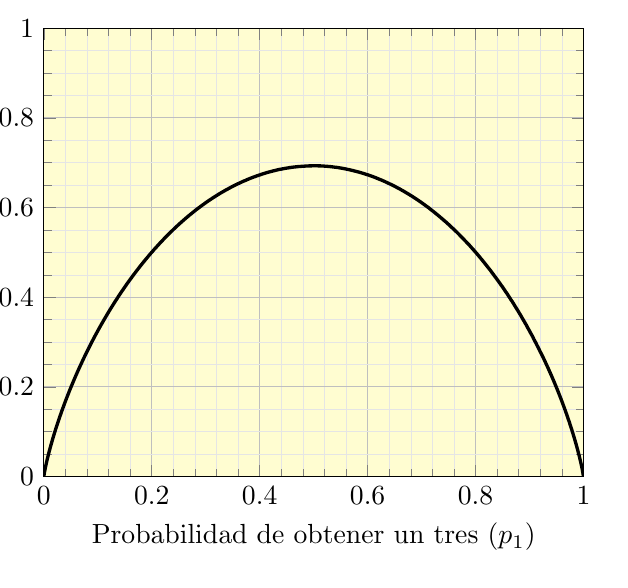
\begin{tikzpicture}[scale=1.00]
\begin{axis}[
	axis background/.style={fill=yellow!18},
	grid style={line width=.2pt,draw=gray!20},
	major grid style={line width=.3pt,draw=gray!50},
	grid=both,
	%enlargelimits={abs=0.5},
	%enlarge x limits=0.0,
	restrict x to domain=0:1,
	%title= CONVERSIÓN EN EL EQUILIBRIO Y TEMPERATURA,
	ylabel style={overlay},
	yticklabel style={overlay},
	%xlabel={$X_{\ce{H2}}$},
	%ylabel={Concentración (\si{\molar})},
	xlabel={Probabilidad de obtener un tres $(p_1)$},
	ylabel={Entropía $(S)$}, %legend style={at={(0.5,0.97)},
	%   anchor=north, legend columns=-1},
	domain=0:1,
	minor y tick num = 3,
	minor x tick num = 4,
	xmin=0,
	xmax=1,
	ymin=0,
	ymax=1,
	%xtick={}
	%ytick={0,20,40,60,80,100,120},
	%grid style={line width=.2pt,draw=gray!20},
	%major grid style={line width=.3pt,draw=gray!50},
	%grid=both
]
\addplot[%
smooth,domain=0:1,color=black,mark=none,samples=500,line width=1.2pt
%] {-x*ln(x)-(1-x)*ln(1-x)};
%] {x*ln((1-x)/x)-ln(1-x)};
% {ln(((1-x)/x)^x)-ln(1-x)};
] {ln((((1-x)/x)^x)/(1-x))};
\end{axis}
\end{tikzpicture}
\caption{Representación gráfica de la entropía de la máquina que produce
  treses y sietes, en función de la probabilidad de obtener un tres.
  Se observa que es máxima cuando $p_1=0,5$.}
\label{fig:entr-p1-S}
\end{figure}


Generalizando a $N$ sucesos probables, la entropía sería máxima cuando
\[
  p_1=p_2=\cdots=p_N = 1/N
\]
\[
  S_{\text{máx}}
  = -\sum_{i} \frac{1}{N} \ln\frac{1}{N}
  = -\frac{1}{N}\,(-\ln N) \sum_i 1
  =  \cancelout{N} \frac{1}{\cancelout{N}}\,\ln N
  = \ln N
\]

Este resultado tiene cierta lógica, porque cuando todos los sucesos fueran
equiprobables, nuestra ignorancia sería máxima. Y si uno de los sucesos
tuviera algo más de probabilidad de ocurrir que otro, entonces tendríamos
mayor grado de conocimiento de lo que se obtendría, y la entropía disminuiría.

El problema de esta conclusión radica en que sólo es válida cuando los sucesos
que se consideren sean disjuntos (u ortogonales). Más adelante se analizará
de una forma más completa.

\section{Traza de una matriz}
La traza de una matriz es la suma de sus elementos diagonales
\[
  \Tr\mmm{A} = \sum_n A_{nn}
\]

\subsection{Propiedades importantes}
Podemos destacar dos propiedades de la traza de matrices:
\begin{enumerate}
\item La traza de la suma de dos matrices es la suma de la traza de
  cada una de ellas
  \begin{equation}\label{eq:entr-traza-de-suma}
    \Tr(\mmm{A} + \mmm{B})
    = \Tr\mmm{A} + \Tr\mmm{B}
  \end{equation}

\item La traza de un escalar por una matriz es el escalar por la traza
  de la matriz
  \begin{equation}\label{eq:entr-traza-escalar-matriz}
    \Tr{(\lambda\mmm{A})}
    = \lambda \Tr\mmm{A}
  \end{equation}
  
\end{enumerate}

\subsection{Traza del producto de dos matrices}
El producto de dos matrices $\mmm{D} = \mmm{A}$ y $\mmm{B}$ se podría
escribir en forma compacta como
\[
  D_{ij} = (AB)_{ij} = \sum_k A_{ik} B_{kj}
\]

Los elementos diagonales de esta matriz serían
\[
  D_{nn} = (AB)_{nn}
\]


La forma compacta de la traza de una matriz $\mmm{D}$ sería la suma
de sus elementos diagonales
\[
  \Tr{\mmm{D}} = \sum_n D_{nn}
\]

La traza del producto de dos matrices sería
\[
  \Tr{(\mmm{A}\mmm{B})} = \sum_n (AB)_{nn} = \sum_n \sum_k A_{nk} B_{kn}
  = \sum_{n,k} A_{nk} B_{kn}
\]

\section{Matriz densidad}
Para estudiar la \emph{matriz densidad} en mecánica cuántica, consideraremos
estados cuánticos con dos grados de libertad, que podremos generalizar
fácilmente a cualquier número $N$ de grados de libertad. No trataremos aquí
con estados con infinitos grados de libertad, que complicarían los cálculos
pero no añadirían nada conceptualmente.

La matriz densidad se utiliza cuando hay \emph{estados mezcla}, que se
estudiarán más adelante.

\subsection{Producto exterior y proyectores}
Sabemos que el producto interno o escalar de dos vectores produce un número
real
\[
  \ket{\phi}\cdot\ket{\psi}
  = \braket{\phi|\psi} \in \symbb{R}
\]

Ahora definimos un producto exterior de dos vectores como
\[
  \ket{\phi}\otimes\ket{\psi}
  = \ket{\phi}\bra{\psi}
\]
que se representa mediante una matriz $N\times N$ en el caso de vectores de un
espacio vectorial de dimensión finita $N$.

Normalmente el producto externo se puede aplicar a un vector columna $\ket{A}$
por la derecha
\[
  \ket{\phi}\bra{\psi} \ket{A}
  = \ket{\phi}\braket{\psi|A}
\]
o bien a un vector fila por la izquierda
\[
  \bra{A} \ket{\phi}\bra{\psi}
  = \braket{A|\phi}\bra{\psi}
\]

El producto externo de un vector de módulo unidad $\ket{\psi}$ por sí mismo se
denomina \emph{proyector} $\ket{\psi}\bra{\psi}$, cuyo resultado al aplicarlo
a un vector $\ket{A}$ es un vector proporcional a $\ket{\psi}$
\[
  \ket{\psi}\bra{\psi} \ket{A}
  = \ket{\psi} \braket{\psi|A}
\]
esto es, proyecta un vector $\ket{A}$ en la dirección definida por
$\ket{\psi}$.

El proyector tiene ciertas propiedades que escribimos sin demostrar:
\begin{itemize}
\item El proyector $\ket{\psi}\bra{\psi}$ es un operador hermítico.
\item El vector $\ket{\psi}$ es un autovector del proyector, con autovalor
  igual a uno
  \[
    \ket{\psi}\bra{\psi} \ket{\psi} = 1 \ket{\psi}
  \]
\item Cualquier vector ortogonal a $\psi$ es autovector del proyector con
  autovalor cero.

  Si $\braket{\psi|\phi} = 0$, entonces
  \[
    \ket{\psi}\bra{\psi} \ket{\phi} = 0 \ket{\phi}
  \]

\item El cuadrado del operador proyector es igual al operador proyector
  \[
    (\ket{\psi}\bra{\psi})^2 = \ket{\psi}\bra{\psi}
  \]

\item La traza de un operador proyector es la suma de sus autovalores
  \[
    \Tr(\ket{\psi}\bra{\psi}) = 1
  \]

\item La suma de los operadores proyección de todos los vectores
  de una base ortonormal es la matriz unidad
  \[
    \sum_{i} \ket{i}\bra{i} = \mmm{I} 
  \]

\item El valor esperado del operador $\mmm{F}$ en el estado $\ket{\psi}$
  es la traza del proyector del vector de estado por el operador $\mmm{F}$
  \begin{equation}\label{eq:entr-valoresperado-como-traza}
    \braket{\mmm{F}} = \braket{\psi|\mmm{F}|\psi}
    = \Tr(\ket{\psi}\bra{\psi} \mmm{F})
  \end{equation}

  Lo demostramos a continuación, recordando que la traza de una matriz es
  la suma de sus elementos diagonales
  $\Tr\mmm{F} = \sum_i \mmm{F}_{ii} = \sum_i \braket{i|\mmm{F}|i}$
  \begin{align*}
    \Tr(\ket{\psi}\bra{\psi} \mmm{F})
    &=
      \sum_i \braket{i|\psi} \braket{\psi|\mmm{F}|i}
      = \sum_i \braket{\psi|\mmm{F}|i} \braket{i|\psi}
      = \sum_i \braket{\psi|\mmm{F}} \ket{i}\bra{i} \ket{\psi}\\
    &=
      \braket{\psi|\mmm{F}} \left(\sum_i\ket{i}\bra{i}\right) \ket{\psi}
      = \braket{\psi|\mmm{F}} \mmm{I} \ket{\psi}
      = \braket{\psi|\mmm{F}|\psi}
      = \braket{\mmm{F}}
  \end{align*}
  
\end{itemize}


\subsection{Definición de matriz densidad}
El estado de un sistema cuántico queda completamente especificado mediante un
vector de estado $\ket{\psi}$, que contiene toda la información que podemos
obtener de él.
Una forma equivalente de especificar el estado de un sistema cuántico
sería mediante la matriz densidad $\mmmg{\rho}$, que se define como
el proyector
\begin{equation}\label{eq:entr-matriz-densidad}
  \mmmg{\rho} = \ket{\psi}\bra{\psi}
\end{equation}

Se puede seguir la evolución dinámica de ambos $\ket{\psi}$ y $\mmmg{\rho}$,
es decir, su evolución con el tiempo.

Una consecuencia de la definición es que la matriz densidad no depende de la
fase global. Supongamos que el vector de estado se escribe como
\[
  \ket{\psi'} = \ket{e^{i\phi}\psi} = e^{i\phi}\ket{\psi}
\]

La matriz densidad no tiene en cuenta la fase global
\[
  \mmmg{\rho}
  = \ket{\psi'}\bra{\psi'}
  = \ket{e^{i\phi}\psi}\bra{e^{i\phi}\psi}
  = e^{i\phi} e^{-i\phi} \ket{\psi}\bra{\psi}
  = \ket{\psi}\bra{\psi}
\]

\subsection{Valor esperado de un observable mecano-cuántico}
Imaginemos que tenemos un sistema cuántico finito\footnotemark{} en un estado
$\ket{\psi}$
\footnotetext{Podríamos considerar también sistemas con infinitas dimensiones,
  en cuyo caso habría que escribir la combinación lineal como una integral
  del tipo $\ket{\psi} = \int dx\,\psi(x) \ket{x}$, pero como no aportaría
  profundidad y sólo se complicaría la notación matemática, nos limitaremos
  a sistemas de dimensiones finitas.}
\[
  \ket{\psi} = a_0 \ket{0} + a_1 \ket{1}
\]
donde hemos representado los vectores de estado que forman la base, $\ket{0}$
y $\ket{1}$, como si fueran \emph{qbits}.

Un \emph{observable} se representa mediante un operador hermítico, que en
el caso de sistemas cuánticos de un número finito de grados de libertad,
se materializan como matrices cuadradas hermíticas
\[
  \mmm{F}^\dagger = \mmm{F}
\]

Hay un teorema que dice que toda matriz hermítica es diagonalizable,
sus valores propios $F_i$ son reales y sus vectores propios
asociados $\ket{F_i}$ forman una base ortonormal.

Además, el \emph{postulado de la medida} establece que al medir $\mmm{F}$,
los valores que se podrán obtener serán los valores propios, con unas ciertas
probabilidades. Y después de obtener uno de ellos $F_i$, el sistema
quedará definido por el estado $\ket{F_i}$ asociado. Las probabilidades de
obtener cada uno de los valores propios en la medida sería
\[
  p_i = |\braket{\psi|F_i}|^2
\]

Como este observable es una matriz, en dos dimensiones sería
\[
  \mmm{F}
  = \begin{pNiceMatrix}
    F_{00} & F_{01}\\
    F_{10} & F_{11}
  \end{pNiceMatrix}
\]

El valor esperado del observable en un estado cuántico $\ket{\psi}$ es
\[
  \braket{\mmm{F}} = \braket{\psi|\mmm{F}|\psi}
\]
que se interpreta como el valor promedio de todos los posibles resultados de
la medida $F_i$, teniendo en cuenta sus probabilidades $p_i$.

Desarrollamos la expresión anterior
\begin{align*}
  \braket{\mmm{F}}
  &=
    \braket{\psi|\mmm{F}|\psi}
    = \begin{pNiceMatrix}
      a_0^* & a_1^*
      \end{pNiceMatrix}
    \begin{pNiceMatrix}
      F_{00} & F_{01}\\
      F_{10} & F_{11}
    \end{pNiceMatrix}
    \begin{pNiceMatrix}
      a_0\\
      a_1
    \end{pNiceMatrix}
    = \begin{pNiceMatrix}
      a_0^* & a_1^*
      \end{pNiceMatrix}
    \begin{pNiceMatrix}
      F_{00} a_0 + F_{01} a_1\\
      F_{10} a_0 + F_{11} a_1
    \end{pNiceMatrix}\\
  &=
    F_{00} a_0 a_0^* + F_{01} a_1 a_0^* + F_{10} a_0 a_1^* + F_{11} a_1 a_1^*\\
  &=
    a_0 a_0^* F_{00} + a_1 a_0^* F_{01} + a_0 a_1^* F_{10} + a_1 a_1^* F_{11}
\end{align*}

Si abreviamos con $\rho_{ij}\equiv a_i a_j^*$, el valor esperado puede
escribirse como
\[
  \braket{\mmm{F}}
  =
  \rho_{00} F_{00} + \rho_{10} F_{01} + \rho_{01} F_{10} + \rho_{11} F_{11}
  = \sum_{n,k} \rho_{nk} F_{kn}
  = \Tr{(\mmmg{\rho}\mmm{F})}
\]

Nótese que el primer factor del producto de matrices depende de las $a_i$,
\begin{equation}\label{eq:entr-elementos-matriz-densidad}
  \rho_{ij} = a_i a_j^*
\end{equation}
que, a su vez, dependen únicamente del estado cuántico del sistema,
$\ket{\psi}$, y que equivale a los elementos de la matriz densidad.
Por otro lado, el segundo factor es la matriz del observable $\mmmg{F}$
que queremos medir, que es independiente del estado.

Por tanto, el valor esperado del observable $\mmm{F}$ es la traza de un
producto de matrices
\begin{equation}\label{eq:entr-valor-esperado-traza}
  \braket{\mmm{F}}
  = \braket{\psi|\mmm{F}|\psi}
  = \Tr{(\mmmg{\rho}\mmm{F})}
\end{equation}
Esto también se puede deducir de la
propiedad~\eqref{eq:entr-valoresperado-como-traza} de los proyectores.

\section{Entropía}
En esta sección utilizaremos una forma más general de calcular la entropía,
la utilizaremos para calcular la en estados puros y mezcla\footnotemark{}
\footnotetext{En el desarrollo de esta sección se pondrán ejemplos de
  estados puros y estados mezcla.}
\begin{equation}\label{eq:entr-def-entropia-general}
  S = -\Tr(\mmmg{\rho}\ln\mmmg{\rho})
\end{equation}
y aprenderemos cuándo equivale a la definición
básica~\eqref{eq:entr-def-entropia-basica}
\[
  S = -\sum_{i} p_i \ln p_i
\]

Empezamos haciendo una serie de consideraciones sobre las implicaciones
acerca del uso de la expresión~\eqref{eq:entr-def-entropia-general}:
\begin{itemize}
\item Hay que destacar que a una misma matriz densidad se puede llegar
  desde infinitos estados mezcla diferentes
  \[
    \mmmg{\rho} = \sum_i w_i \ket{\psi_i}\bra{\psi_i}
  \]
  donde $w_i$ es el peso con que participa cada estado puro
  $\ket{\psi_i}\bra{\psi_i}$, en el estado mezcla.
  
  Pero de esos infinitos estados mezcla sólo hay uno, que escribiremos
  como
  \begin{equation}\label{eq:entr-estados-ortogonales}
    \mmmg{\rho} = \sum_i \lambda_i \ket{u_i}\bra{u_i}
  \end{equation}
  en el que se puede utilizar la definición básica
  ~\eqref{eq:entr-def-entropia-basica}
  \[
    S = -\sum_i\lambda_i\ln\lambda_i
  \]
  y es aquél en el que los estados puros $\ket{u_i}$ que se mezclan
  son \emph{ortogonales}.
  
  Además, cuado los que se mezclan son ortogonales,
  la expresión~\eqref{eq:entr-def-entropia-basica} se minimiza, esto es
  \[
    S < -\sum_i w_i\ln w_i
  \]

  Para obtener la mezcla de estados
  ortogonales~\eqref{eq:entr-estados-ortogonales} a partir de cualquier
  matriz densidad $\mmmg{\rho}$, hay que escribir esta última en su base
  propia, es decir, hay que diagonalizarla.
  Por tanto debemos hallar los valores propios $\lambda_i$ de la matriz.
  Esto se debe a que
  \emph{los vectores propios} $\ket{u_i}$ \emph{son ortogonales} y se
  corresponden con los estados que se mezclan.

\item Lo anterior se puede explicar matemáticamente, en parte, debido a la
  necesidad de calcular el logaritmo de la matriz densidad. El logaritmo de
  una matriz $\mmmg{\rho}$ se puede desarrollar en serie de potencias de
  $\mmmg{\rho} - \mmm{I}$, siempre que la serie sea convergente
  \begin{align*}
    \ln\mmmg{\rho}
    &=
      \mmmg{I}
      + \frac{\mmmg{\rho} - \mmmg{I}}{1!}
      + \frac{(\mmmg{\rho} - \mmmg{I})^2}{2!}
      + \frac{(\mmmg{\rho} - \mmmg{I})^3}{3!}
      + \cdots
  \end{align*}
  
  El logaritmo de una matriz cuadrada se puede hallar en la práctica utilizando
  la propiedad de que el logaritmo de una matriz diagonal es la matriz de los
  logaritmos de sus elementos diagonales.
  Por ejemplo, diagonalizando $\mmmg{\rho}$ en dos dimensiones
  \[
    \mmmg{\rho}
    = \begin{pNiceMatrix}
      \lambda_0 & 0\\
      0 & \lambda_1
    \end{pNiceMatrix}
    \hspace{.5em}\longrightarrow\hspace{.5em}
    \ln\mmmg{\rho}
    = \begin{pNiceMatrix}
      \ln\lambda_0 & 0\\
      0 & \ln\lambda_1
    \end{pNiceMatrix}
  \]
  y como resulta que la matriz densidad es hermítica, tenemos la seguridad de
  que se puede diagonalizar.
  
  Entonces, y sólo entonces
  \[
    \mmmg{\rho}\ln\mmmg{\rho}
    = \begin{pNiceMatrix}
      \lambda_0 & 0\\
      0 & \lambda_1
    \end{pNiceMatrix}
    \begin{pNiceMatrix}
      \ln\lambda_0 & 0\\
      0 & \ln\lambda_1
    \end{pNiceMatrix}
    = \begin{pNiceMatrix}
      \lambda_0\ln\lambda_0 & 0\\
      0 & \lambda_1\ln\lambda_1
      \end{pNiceMatrix}
    \]
    la entropía se podría expresar mediante la fórmula
    básica~\eqref{eq:entr-def-entropia-basica}
    \[
      S = -\Tr(\mmmg{\rho}\ln\mmmg{\rho})
      = -\lambda_0\ln\lambda_0 - \lambda_1\ln\lambda_1
    \]
    donde las $\lambda_i$ son los pesos de los estados mezcla ortogonales
    $\ket{u_0}$ y $\ket{u_1}$.
\end{itemize}


\subsection{Estados puros}
Se dice que un sistema se encuentra en un \emph{estado puro} cuando se
conoce perfectamente. Esto tiene distintas consecuencias según el sistema
sea clásico o cuántico.

La entropía de estos sistemas vale cero porque nuestro grado de desconocimiento
es nulo
\[
  S = 0
\]

\subsubsection{Mecánica clásica}
En mecánica clásica, un estado puro se representa mediante un punto en el
espacio de las fases. El estado, en un instante $t$, de una partícula queda
completamente determinado mediante sus coordenadas $\vvv{r}$ y su momento
lineal $\vvv{p}$.
Conocer el estado de un sistema clásico en un tiempo $t$, implica conocerlo
en cualquier instante posterior siempre que tengamos en cuenta las fuerzas que
actúan sobre el sistema y las ligaduras que constriñen su movimiento.

Los estados posibles que resultan de lanzar una moneda\footnotemark{} son dos
puntos en el espacio de fases: \emph{cara} y \emph{cruz}, que podríamos
describir por $0$ y $1$, respectivamente.
\footnotetext{Descartando la posibilidad de que quede de canto.}
Estos dos estados son mútuamente excluyentes en el sentido de que si una
moneda se encuentra, por ejemplo, en el estado \emph{cara}, es imposible
que la veamos como \emph{cruz}, y viceversa. Diremos que estos estados
son ortogonales.

Si una persona lanza una moneda y nos comunica el resultado, por ejemplo,
\emph{cara} o $0$, la moneda se encontrará en un estado puro que no cambiará
mientras no se interactúe con la moneda para cambiarlo.
Así, cada vez que midamos su estado, encontraremos que está de cara o $0$
siempre, con una probabilidad $p=1$.

La entropía se puede calcular de las dos formas:
\begin{itemize}
\item En estas condiciones, la entropía de la moneda será cero
\[
  S = -p_0\ln p_0 - p_1\ln p_1 = -1 \ln 1 - 0\ln 0 = 0
\]
lo que significa que nuestro grado de desconocimiento de su estado es cero,
lo que implica que está en un estado clásico puro.

\item Por otro lado, como al lanzar la moneda son posibles los valores,
cara $(1, 0)$ y cruz $(0,1)$.
Si sale cara, por ejemplo, el vector de estado de la moneda será
\[
  \ket{0} =
  \begin{pNiceMatrix}
    1\\
    0
  \end{pNiceMatrix}
\]

La matriz de densidad es
\[
  \mmmg{\rho}
  = \ket{0}\bra{0}
  = \begin{pNiceMatrix}
    1\\
    0
  \end{pNiceMatrix}
  \begin{pNiceMatrix}
    1 & 0
  \end{pNiceMatrix}
  = \begin{pNiceMatrix}
    1 & 0\\
    0 & 0
  \end{pNiceMatrix}
\]

Esta matriz es diagonal, calculamos su logaritmo directamente y lo
multiplicamos por la matriz.
Pero no intentamos resolver el logaritmo de cada elemento hasta que no
multipliquemos las matrices
\[
  \mmmg{\rho}\ln\mmmg{\rho}
  =
  \begin{pNiceMatrix}
    1 & 0\\
    0 & 0
  \end{pNiceMatrix}
  \begin{pNiceMatrix}
    \ln 1 & 0\\
    0 & \ln 0
  \end{pNiceMatrix}
  =
  \begin{pNiceMatrix}
    1\ln 1 & 0\\
    0 & 0\ln 0
  \end{pNiceMatrix}
\]

La entropía será la traza de la matriz
\[
  S
  = -\Tr(\mmmg{\rho}\ln\mmmg{\rho})
  = -1\ln 1 - 0\ln 0
  = 0
\]
\end{itemize}


\subsubsection{Mecánica cuántica}
Consideraremos, por sencillez, un sistema cuántico de dos dimensiones, como
puede ser el spin 1/2. Si se mide el spin de una partícula en una
cierta dirección, que llamaremos eje $z$, el resultado será un spin
\emph{hacia arriba} o \emph{hacia abajo}, de acuerdo con el postulado
de la medida. En el primer caso, la partícula quedará en el estado que
representaremos como $\ket{0}=\ket{z_+}$, y en el segundo en
$\ket{1}=\ket{z_-}$, donde hemos utilizado esta vez el $0$ y el $1$ por
analogía con los \emph{qbits}, y porque además, al representarlos mediante
números se podrían utilizar como índices de sumatorios en fórmulas.

Según este postulado, los posibles valores que se pueden obtener (en este
ejemplo dos) se corresponden con estados que son ortogonales entre sí,
esto es, su producto interno es nulo
\[
  \braket{0|1} = \braket{1|0} = 0
\]
Esto se puede interpretar como que los dos estados son
\emph{mútuamente excluyentes},
es decir, si una partícula estuviera en un instante en uno de los dos estados,
por ejemplo $\ket{0}$, sería imposible encontrarla con spin hacia abajo en el
mismo instante\footnotemark{}.
\footnotetext{Si su estado cambiara con el tiempo, sí podría ser posible
  encontrarla más tarde con el spin opuesto.}

La entropía de un sistema cuántico se define en función de la matriz densidad
\[
  S = -\Tr(\mmmg{\rho}\ln\mmmg{\rho})
\]

Cuando consideramos el spin 1/2, la matriz densidad será una matriz
cuadrada $2\times 2$. Un \emph{estado puro} genérico de spin 1/2 de un sistema,
tendría la forma
\[
  \ket{\psi} = a_0\ket{0} + a_1\ket{1}
  = a_0
  \begin{pNiceMatrix}
    1\\
    0
  \end{pNiceMatrix}
  + a_1
  \begin{pNiceMatrix}
    0\\
    1
  \end{pNiceMatrix}
  = \begin{pNiceMatrix}
    a_0\\
    a_1
  \end{pNiceMatrix}
\]

Las amplitudes de probabilidad $a_0$ y $a_1$ nos permiten calcular las
probabilidades de obtener los dos valores posibles del spin en la dirección del
eje $z$, asociados a los estados $\ket{0}$ y $\ket{1}$
\begin{align*}
  p_0 &= a_0 a_0^* = |a_0|^2\\
  p_1 &= a_1 a_1^* = |a_1|^2
\end{align*}

La matriz densidad sería
\begin{equation}\label{eq:entr-matriz-densidad-spin1/2}
  \mmmg{\rho}
  =
  \ket{\psi}\bra{\psi}
  = \begin{pNiceMatrix}
    a_0\\
    a_1
  \end{pNiceMatrix}
  \begin{pNiceMatrix}
    a_0^* & a_1^*
  \end{pNiceMatrix}
  = \begin{pNiceMatrix}
    a_0 a_0^* & a_0 a_1^*\\
    a_1 a_0^* & a_1 a_1^*
  \end{pNiceMatrix}
  = \begin{pNiceMatrix}
    p_0 & a_0 a_1^*\\
    a_1 a_0^* & p_1
    \end{pNiceMatrix}
\end{equation}

Para calcular el logaritmo de la matriz densidad, aprovechamos que
la matriz densidad es hermítica, por lo que sus valores propios serán números
reales no negativos debido a que los valores diagonales son probabilidades.
Una vez diagonalizada, el logaritmo de la matriz sería la matriz de los
logaritmos de los elementos diagonales\footnotemark{}.
\footnotetext{Posteriormente habría que reescribir esta matriz diagonal con
  logaritmos en la base original y multiplicarla por la matriz densidad
  original, pero no necesitaremos hacerlo porque para calcular la entropía
  necesitamos la traza, que sería igual en las dos matrices.}

Supongamos que la hemos diagonalizado y la representamos en la base de
los vectores propios
\[
  \mmmg{\rho}'
  = \begin{pNiceMatrix}
    \lambda_0 & 0\\
    0 & \lambda_1
  \end{pNiceMatrix}
\]

Entonces el logaritmo de la matriz sería
\[
  \ln\mmmg{\rho}'
  = \begin{pNiceMatrix}
    \ln\lambda_0 & 0\\
    0 & \ln\lambda_1
  \end{pNiceMatrix}
\]

Si alguna de las probabilidades $\lambda_i$ fuera cero, su logaritmo no
estaría definido. Pero como lo que necesitamos es $\mmmg{\rho}'\ln\mmmg{\rho}'$,
entonces podremos suponer, como se vió en la
sección~\ref{subsect:entr-entropia-basica} que
\begin{equation}\label{eq:entr-0ln0}
  "0\ln 0" = \lim_{p_i\to 0} p_i\ln p_i = 0
\end{equation}

Por tanto escribimos $\mmmg{\rho}'\ln\mmmg{\rho}'$, obviando de momento
el que algún $p_i'$ fuera cero
\[
  \mmmg{\rho}'\ln\mmmg{\rho}'
  = \begin{pNiceMatrix}
    \lambda_0 & 0\\
    0 & \lambda_1  
  \end{pNiceMatrix}
  \begin{pNiceMatrix}
    \ln \lambda_0 & 0\\
    0 & \ln \lambda_1
  \end{pNiceMatrix}
  = \begin{pNiceMatrix}
    \lambda_0\ln \lambda_0 & 0\\
    0 & \lambda_1\ln \lambda_1
  \end{pNiceMatrix}
\]

El opuesto de la traza de esta matriz sería
\[
  -\Tr(\mmmg{\rho}'\ln\mmmg{\rho}')
  = -\lambda_0\ln \lambda_0 - \lambda_1\ln \lambda_1
\]

Aprovechando que al diagonalizar una matriz se conserva la traza,
la entropía del sistema sería, finalmente
\begin{equation}\label{eq:entr-entropia-cuantica-p0'-p1'}
  S = -\Tr(\mmmg{\rho}\ln\mmmg{\rho})
  = -\Tr(\mmmg{\rho}'\ln\mmmg{\rho}')
  = -\lambda_0\ln \lambda_0 - \lambda_1\ln \lambda_1
\end{equation}

Para nuestro sistema de spin 1/2, diagonalizamos la matriz
densidad~\eqref{eq:entr-matriz-densidad-spin1/2}, planteando su ecuación
de autovalores y autovectores
\[
  \mmmg{\rho} \vvv{u} = \lambda \vvv{u}
\]
\[
  \mmmg{\rho} \vvv{u} - \lambda \vvv{u} = \vvv{0}
\]
\[
  (\mmmg{\rho} - \lambda\mmm{I}) \vvv{u} = \vvv{0}
\]
\begin{align*}
  \begin{pNiceMatrix}
    p_0 - \lambda & a_0 a_1^*\\
    a_1 a_0^* & p_1 - \lambda
  \end{pNiceMatrix}
  \begin{pNiceMatrix}
    u\\
    v
  \end{pNiceMatrix}
  =
  \begin{pNiceMatrix}
    0\\
    0
  \end{pNiceMatrix}
\end{align*}

Para obtener los valores propios, el determinante de la matriz debe anularse,
ya que el sistema de ecuaciones tiene que ser compatible indeterminado
\[
  \begin{vNiceMatrix}
    p_0 - \lambda & a_0 a_1^*\\
    a_1 a_0^* & p_1 - \lambda
  \end{vNiceMatrix}
  = 0
\]

Desarrollando el determinante, obtenemos la ecuación característica, y
teniendo en cuenta que $p_0 + p_1 = 1$
\[
  \left(p_0-\lambda\right) \left(p_1-\lambda\right) -
  a_0 a_1^* a_1 a_0^*
  = 0
\]
\[
  \cancelout{p_0 p_1} - (p_0 + p_1)\lambda + \lambda^2 - \cancelout{p_0 p_1} = 0
\]
\[
  \lambda^2 - \lambda = 0
\]
\[
  \lambda(\lambda - 1) = 0
\]
de donde $\lambda_0 = 1$ y $\lambda_1 = 0$.
La matriz densidad diagonalizada será
\[
  \mmmg{\rho}
  = \begin{pNiceMatrix}
    1 & 0\\
    0 & 0
  \end{pNiceMatrix}
\]

Y según~\eqref{eq:entr-entropia-cuantica-p0'-p1'}, junto
con~\eqref{eq:entr-0ln0}, la entropía del sistema puro $\ket{\psi}$ será cero
\[
  S = -\lambda_0\ln \lambda_0 - \lambda_1\ln \lambda_1
  = -1\ln 1 - 0\ln 0
  = 0
\]
lo que implica que se el estado está completamente determinado por el
vector de estado $\ket{\psi}$. Nótese que el hecho de que no sepamos
con seguridad el resultado de una medida del spin en la dirección $z$,
\emph{es inherente a la mecánica cuántica} y no se debe a ningún
desconocimiento achacable a nosotros.


\subsection{Estados mezcla}
Los \emph{estados mezcla} surgen debido a un \emph{conocimiento incompleto}
del estado de un sistema. Suelen aparecer en mecánica estadística, tanto
clásica como cuántica, porque debido al gran número de partículas implicadas
resulta del todo imposible conocer el estado de todas y cada una de ellas.
También se tienen que tener en cuenta los estados mezcla cuando un sistema
cuántico conocido interacciona con el ambiente de forma incontrolable y por
decoherencia nos hace perder información.

En mecánica cuántica hay solapamientos, y por solapamiento nos referimos a
que no hay un experimento que pueda distinguir entre dos estados no
ortogonales.
Una medida en un estado mezcla nos permite distinguir sólo entre estados
ortogonales; recuérdese que el resultado de la medida de un observable da como
resultado uno de los valores propios de éste.
Pero estos valores propios están asociados a vectores propios ortogonales entre
sí, que se corresponden a estados ortogonales\footnotemark{}.
\footnotetext{Hay técnicas que intentan minimizar el error que se produce al
  intentar distinguir entre estados solapados
  (\emph{quantum measure discrimination}).}

\begin{quote}
  ``Para caracterizar estados mezcla debemos utilizar la matriz densidad
  $\mmmg{\rho}$, pues ya no se puede utilizar el rayo en el espacio de Hilbert
  que representa a un estado puro $\ket{\psi}$''
\end{quote}

Hay infinitas mezclas de estados que producen la misma matriz densidad
(mismo estado), y así, todas ellas son \emph{físicamente indistiguibles}.
Además ocurre que ningún experimento puede discriminar entre estados no
ortogonales.
De éstas, sólo hay una mezcla que implica estados ortogonales $\ket{u_i}$
y sus probabilidades $\lambda_i$, que reproduce la matriz densidad.
Entonces, al realizar una medida en ese estado $\mmmg{\rho}$, en realidad
estamos disciminando entre estos estados ortogonales.

¿Cómo podemos encontrar los estados $\ket{u_i}$ y sus probabilidades
asociadas $\lambda_i$?
Diagonalizando la matriz, esto es, expresándola en función de la
base formada por sus vectores propios.

Además se produce la circunstancia de que el cálculo con los valores propios
es el que produce el menor valor, y éste valor es la entropía
\[
  S = -\sum_i \lambda_i\ln\lambda_i
\]
mientras que si tomáramos los pesos de cualquiera de los otros posibles
estados mezcla que reproducen $\mmmg{\rho}$, el valor sería mayor que la
entropía
\[
  -\sum_i w_i\ln w_i > S
\]

Como en esta sección nos interesa la entropía, tendremos que
calcularla mediante
\[
  S = - \Tr(\mmmg{\rho}\ln\mmmg{\rho})
\]

Cuando los estados que se mezclan son ortonormales, la fórmula anterior
es equivalente a
\[
  S = -\sum_i \lambda_i\ln \lambda_i
\]
    
\subsubsection{Construcción de la matriz densidad de un estado mezcla}
Supongamos una mezcla de dos estados que no tienen porqué ser ortogonales,
\begin{align*}
  \ket{\psi_0} &= a_0 \ket{0} + a_1 \ket{1}\\
  \ket{\psi_1} &= b_0 \ket{0} + b_1 \ket{1}
\end{align*}
donde $\ket{0}$ y $\ket{1}$ forman una base ortonormal.

El valor esperado del observable $\mmm{F}$ en cada uno de los estados sería,
según~\eqref{eq:entr-valor-esperado-traza}
\begin{align*}
  \braket{\mmm{F}}_0
  &=
    \braket{\psi_0|\mmm{F}|\psi_0} = \Tr{(\mmmg{\rho_0} \mmm{F})}\\
  \braket{\mmm{F}}_1
  &=
    \braket{\psi_1|\mmm{F}|\psi_1} = \Tr{(\mmmg{\rho_1} \mmm{F})}
\end{align*}
Como $\mmmg{\rho}$ depende del estado, le ponemos un subíndice $\mmmg{\rho_i}$
para indicar el estado $\ket{\psi_i}$ con el que se corresponde.

Si alguien nos dice que el sistema está descrito por $\ket{\psi_0}$ con
un peso\footnotemark{} $w_0$ y por $\ket{\psi_1}$ con un peso $w_1$,
donde los estados no son necesariamente ortogonales, entonces el valor
esperado de $\mmm{F}$ para el sistema en esta situación sería
\footnotetext{Le podemos llamar probabilidad, pero como no se refiere
  a un estado puro preferimos utilizar otro nombre.}
\[
  \braket{\mmm{F}}
  = w_0 \braket{\mmm{F}}_0 + w_1 \braket{\mmm{F}}_1
  = w_0 \braket{\psi_0|\mmm{F}|\psi_0} + w_1 \braket{\psi_1|\mmm{F}|\psi_1}
\]
y esto es así porque al incluir los valores esperados para cada posible estado
del sistema $\braket{\mmm{F}}_i = \braket{\psi_i|\mmm{F}|\psi_i}$ ya se han
promediado las incertidumbres cuánticas y estamos trabajando de forma
estadística normal, \emph{por encima de lo cuántico}.

Vayamos un poco más alla a ver si llegamos a alguna conclusión que implique
a la matriz densidad. Aplicamos las
propiedades~\eqref{eq:entr-traza-de-suma}
y~\eqref{eq:entr-traza-escalar-matriz}
de la traza de matrices
\begin{align*}
  \braket{\mmm{F}}
  &=
    w_0 \braket{\psi_0|\mmm{F}|\psi_0} + w_1 \braket{\psi_1|\mmm{F}|\psi_1}
    = w_0 \Tr{(\mmmg{\rho_0}\mmm{F})} + w_1 \Tr{(\mmmg{\rho_1}\mmm{F})}\\
  &=
    \Tr{(w_0 \mmmg{\rho_0}\mmm{F})} + \Tr{(w_0 \mmmg{\rho_1}\mmm{F})}
    = \Tr{\left[w_0\mmmg{\rho_0}\mmm{F} + w_1\mmmg{\rho_1}\mmm{F}\right]}\\
  &=
    \Tr{\left[(w_0\mmmg{\rho_0} + w_1\mmmg{\rho_1}) \mmm{F}\right]}
\end{align*}

Comparando el segundo miembro de la expresión anterior
con~\eqref{eq:entr-valor-esperado-traza}, vemos que
$w_0\mmmg{\rho_0} + w_1\mmmg{\rho_1}$ sería la matriz densidad de un
\emph{estado mezcla} formado por varios estados puros $\ket{\psi_0}$ y
$\ket{\psi_1}$, con pesos respectivos $w_0$ y $w_1$.

Por tanto definimos un estado mezcla $\mmmg{\rho}$ como
\begin{equation}\label{eq:entr-estado-mezcla-rho}
  \mmmg{\rho} = w_0\mmmg{\rho_0} + w_1\mmmg{\rho_1}
\end{equation}

Con estados puros no se necesita el formalismo de la matriz densidad, pero
con estados mezclas es obligatorio.

Estos estados mezcla pueden surgir en física estadística, por ejemplo, donde
existe la posibilidad de haya distintos estados de energía posibles,
como $\ket{E_0}$, $\ket{E_1}$, etc., que se pueden ocupar por las partículas
del sistema con unos ciertos pesos o probabilidades $w_0$, $w_1$, etc.,
que dependen de la temperatura. La energía total del sistema contempla esa
mezcla de estados $\ket{E_i}$ (que se llaman estados de Gibbs).
Por tanto, para describir la termodinámica y la cuántica se necesitan estados
mezcla. También se necesitan los estados mezcla en cosas tan avanzadas como
entrelazamiento en el espacio-tiempo.

\subsubsection{Experimentos clásicos}
Vamos a proponer dos experimentos clásicos:
\begin{enumerate}
\item El primer experimento se mezclan estados ortogonales.
  
    Supongamos que alguien a quien no vemos, quizás por estar tras una
    pantalla, utiliza un sistema clásico que podría ser una moneda o cualquier
    otro dispositivo. Prepara un juego que pueda producir dos resultados, que
    llamaremos cara y cruz, y que denotaremos como 0 o 1. Supongamos que se
    trata de una moneda trucada que produce cara en un cuarto de los
    lanzamientos y cruz en tres cuartos de ellos, circunstancia de la que
    nos informa de antemano.

    Entonces, lanza la moneda y produce un resultado que nosotros no podemos
    ver y por tanto tenemos un cierto grado de ignorancia, aunque cualquier
    otra persona que estuviera con la anterior podrá conocerlo.
    Este es un ejemplo de ignoracia clásica, debido a que no conocemos el
    resultado del lanzamiento de la moneda.

    Como los dos estados posibles del experimento son ortogonales, lo
    resolveremos de dos formas:
    \begin{itemize}
    \item Calculamos mediante~\eqref{eq:entr-def-entropia-basica}
      nuestro grado de desconocimiento del estado de la moneda
      \[
        S
        = -p_0\ln p_0 - p_1\ln p_1
        = -\frac{1}{4}\,\ln\frac{1}{4} - \frac{3}{4}\ln\frac{3}{4}
        = 0,5623\cdots
      \]

    \item Seguimos el camino más elaborado que utiliza la matriz densidad.

      Los dos estados que se mezclan son
      \[
        \ket{\psi_0}
        =
        \ket{0}
        =
        \begin{pNiceMatrix}
          1\\
          0
        \end{pNiceMatrix}
        \hspace{.5em}\text{y}\hspace{.5em}
        \ket{\psi_1}
        =
        \ket{1}
        =
        \begin{pNiceMatrix}
          0\\
          1
        \end{pNiceMatrix}
      \]
      donde $\ket{0}$ representa cara y $\ket{1}$ cruz.

      La matriz densidad que describe la mezcla es
      \begin{align*}
        \mmmg{\rho}
        &=
          w_0\mmmg{\rho_0} + w_1\mmmg{\rho_1}
          = w_0\ket{0}\bra{0} + w_1\ket{1}\bra{1}\\
        &=
          \frac{1}{4}
          \begin{pNiceMatrix}
            1\\
            0
          \end{pNiceMatrix}
        \begin{pNiceMatrix}
          1 & 0
        \end{pNiceMatrix}
        + \frac{3}{4}
        \begin{pNiceMatrix}
          0\\
          1
        \end{pNiceMatrix}
        \begin{pNiceMatrix}
          0 & 1
        \end{pNiceMatrix}
        =
          \begin{pNiceMatrix}
            1/4 & 0\\
            0 & 3/4
          \end{pNiceMatrix}
      \end{align*}

      La matriz densidad es diagonal, por lo que se puede calcular
      fácilmente el logaritmo de la matriz, multiplicarlo por la matriz
      densidad, hallar la traza y calcular su entropía
      \[
        S
        = -\Tr(\mmmg{\rho}\ln\mmmg{\rho})
        = -\frac{1}{4}\ln\frac{1}{4} - \frac{3}{4}\ln\frac{3}{4}
        = 0,5623\cdots
      \]
    \end{itemize}

  \item Un ejemplo de mezcla de estados no ortogonales consiste en el
    lanzamiento de un dado, el primer estado es que salga un dos
    y el otro que salga un número par. Obviamente los dos estados no
    son disjuntos, por lo que no se puede utilizar la fórmula básica.

    La probabilidad de que salga un dos es $1/6$, mientras
    la de que salga un número par es $3/6 = 1/2$.
    El estado mezcla sería algo así
    \[
      \begin{array}{lll}
        \ket{\psi_1} && w_1 = 1/6\\[4pt]
        \ket{\psi_2} && w_2 = 1/2\\
      \end{array}
    \]
    
    Los vectores normalizados implicados son
    {\small
      \[
        \ket{\psi_1}
        = \begin{pNiceMatrix}
          0\\
          1\\
          0\\
          0\\
          0\\
          0
        \end{pNiceMatrix}
        \hspace{1.5em}\text{y}\hspace{1.5em}
        \ket{\psi_2}
        = \frac{1}{\sqrt{3}}
        \begin{pNiceMatrix}
          0\\
          1\\
          0\\
          1\\
          0\\
          1
        \end{pNiceMatrix}      
      \]
    }
    
    Construimos la matriz densidad de los estados individuales
    {\small
      \begin{align*}
        \mmmg{\rho_1}
        &=
          \ket{\psi_1}\bra{\psi_1}
          = \begin{pNiceMatrix}
            0\\
            1\\
            0\\
            0\\
            0\\
            0
          \end{pNiceMatrix}
        \begin{pNiceMatrix}
          0 & 1 & 0 & 0 & 0 & 0
        \end{pNiceMatrix}
      = \begin{pNiceMatrix}
        0 & 0 & 0 & 0 & 0 & 0\\
        0 & 1 & 0 & 0 & 0 & 0\\
        0 & 0 & 0 & 0 & 0 & 0\\
        0 & 0 & 0 & 0 & 0 & 0\\
        0 & 0 & 0 & 0 & 0 & 0\\
        0 & 0 & 0 & 0 & 0 & 0
      \end{pNiceMatrix}\\
        \mmmg{\rho_2}
        &=
          \ket{\psi_2}\bra{\psi_2}
          = \frac{1}{\sqrt{3}}
          \begin{pNiceMatrix}
            0\\
            1\\
            0\\
            1\\
            0\\
            1
          \end{pNiceMatrix}
        \frac{1}{\sqrt{3}}
        \begin{pNiceMatrix}
          0 & 1 & 0 & 1 & 0 & 1
        \end{pNiceMatrix}
        = \frac{1}{3}
        \begin{pNiceMatrix}
          0 & 0 & 0 & 0 & 0 & 0\\
          0 & 1 & 0 & 1 & 0 & 1\\
          0 & 0 & 0 & 0 & 0 & 0\\
          0 & 1 & 0 & 1 & 0 & 1\\
          0 & 0 & 0 & 0 & 0 & 0\\
          0 & 1 & 0 & 1 & 0 & 1
        \end{pNiceMatrix}                      
      \end{align*}
    }
    
    La matriz densidad del estado mezcla sería
    {\small
      \begin{align*}
        \mmmg{\rho}
        &=
          w_0\mmmg{\rho_1} + w_1\mmmg{\rho_2}
          = \frac{1}{6}\mmmg{\rho_1} + \frac{1}{2}\mmmg{\rho_2}\\
        &=
          \frac{1}{6}
          \begin{pNiceMatrix}
            0 & 0 & 0 & 0 & 0 & 0\\
            0 & 1 & 0 & 0 & 0 & 0\\
            0 & 0 & 0 & 0 & 0 & 0\\
            0 & 0 & 0 & 0 & 0 & 0\\
            0 & 0 & 0 & 0 & 0 & 0\\
            0 & 0 & 0 & 0 & 0 & 0
          \end{pNiceMatrix}
        + \frac{1}{2}\cdot\frac{1}{3}
        \begin{pNiceMatrix}
          0 & 0 & 0 & 0 & 0 & 0\\
          0 & 1 & 0 & 1 & 0 & 1\\
          0 & 0 & 0 & 0 & 0 & 0\\
          0 & 1 & 0 & 1 & 0 & 1\\
          0 & 0 & 0 & 0 & 0 & 0\\
          0 & 1 & 0 & 1 & 0 & 1
        \end{pNiceMatrix}\\
        &= \frac{1}{6}
          \begin{pNiceMatrix}
            0 & 0 & 0 & 0 & 0 & 0\\
            0 & 2 & 0 & 1 & 0 & 1\\
            0 & 0 & 0 & 0 & 0 & 0\\
            0 & 1 & 0 & 1 & 0 & 1\\
            0 & 0 & 0 & 0 & 0 & 0\\
            0 & 1 & 0 & 1 & 0 & 1
          \end{pNiceMatrix}
      \end{align*}
    }
    
    Los valores propios son
    \[
      \lambda_1 = \frac{2-\sqrt{2}}{6}
      ;\hspace{.25em} \lambda_2 = \frac{2+\sqrt{2}}{6}
      ;\hspace{.25em} \lambda_3 = \lambda_4 = \lambda_5 = \lambda_6 = 0
    \]
    
    Por tanto, la entropía sería
    \begin{align*}
      S
      &=
      -\Tr(\mmmg{\rho}\ln\mmmg{\rho})
      = -\sum_{i=1}^6 \lambda_i \ln\lambda_i\\
      &= - \frac{2-\sqrt{2}}{6}\ln\frac{2-\sqrt{2}}{6}
        - \frac{2+\sqrt{2}}{6}\ln\frac{2+\sqrt{2}}{6}
        + 0 + 0 + 0 + 0\\
      &=
        0,54797\cdots
    \end{align*}

    Obsérvese que si hubiéramos realizado el cálculo incorrecto, hubiera
    dado un resultado mayor
    \[
      -w_1\ln w_1 - w_2\ln w_2
      = -\frac{1}{6} \ln\frac{1}{6} - \frac{1}{2}\ln\frac{1}{2}
      = 0,57762\cdots
    \]
    
    En la sección~\ref{sect:apcua-estadomezcla-dado} del
    apéndice~\ref{chapt:apcua-matriz-densidad-codigo} se lista el código
    para calcular los valores de este ejemplo.
\end{enumerate}



%%% Local Variables:
%%% coding: utf-8
%%% mode: latex
%%% TeX-engine: luatex
%%% TeX-master: "../cuarentena.tex"
%%% End:


%\include{./texto/entropia-de-entrelazamiento}

% -----------------------------------------------------------------------------
% Apéndices
\backmatter
%\part{Apéndices}
\appendix
\renewcommand{\thechapter}{A}
\clearpage
% apdca.tex
%
% Copyright (C) 2022-2025 José A. Navarro Ramón <janr.devel@gmail.com>
% 1) Código LuaLatex:
%    Licencia GPL-2.
% 2) Producto en pdf, postscript, etc.:
%    Licencia Creative Commons Recognition Share alike. (CC-BY-SA)

\chapter{Vectores y valores propios de las matrices de Pauli}
\label{chapt:apcA-eigenvalues-eigenvectors-Pauli}

\section{Procedimiento para obtener vectores y valores propios}
Supongamos la matriz genérica $\mmm{\sigma_i}$, $i=1,2,3$.
La ecuación de autovalores y autovectores es
\[
  \mmm{\sigma_i} \vvv{v} = \lambda \vvv{v}
\]
\[
  \mmm{\sigma_i} \vvv{v} - \lambda \mmm{I}\vvv{v} = \vvv{0}
\]
\begin{equation}\label{eq:apcA-eigen-general}
  [\mmm{\sigma_i} -\lambda\mmm{I}] \vvv{v} = \vvv{0}
\end{equation}

A continuación aplicamos esta ecuación a cada matriz de Pauli.

\subsection{Primera matriz de Pauli}
\label{sect:apcA-Pauli-sigma1}
Desarrollamos la expresión \eqref{eq:apcA-eigen-general} para la primera
matriz de Pauli, $\mmm{\sigma_1}$
\[
  \left[
  \begin{pNiceMatrix}
    0 & 1\\
    1 & 0
  \end{pNiceMatrix}
  -
  \begin{pNiceMatrix}
    \lambda & 0\\
    0 & \lambda
  \end{pNiceMatrix}
\right]
\begin{pNiceMatrix}
  v_1\\
  v_2
\end{pNiceMatrix}
=
\begin{pNiceMatrix}
  0\\
  0
\end{pNiceMatrix}
\]
\[
  \begin{pNiceMatrix}
    -\lambda & 1\\
    1 & -\lambda
  \end{pNiceMatrix}
\begin{pNiceMatrix}
  v_1\\
  v_2
\end{pNiceMatrix}
=
\begin{pNiceMatrix}
  0\\
  0
\end{pNiceMatrix}
\]
\[
  \begin{pNiceMatrix}
    -\lambda v_1 + v_2\\
    v_1 - \lambda v_2
  \end{pNiceMatrix}
  =
\begin{pNiceMatrix}
  0\\
  0
\end{pNiceMatrix}
\]
Tenemos dos ecuaciones con tres incógnitas
\begin{equation}\label{eq:apcA-ecs-sigma1}
  \left\{
    \begin{array}{r@{}r@{}r@{}r@{}}
      -\lambda v_1 & {} + {} & v_2 & {} = 0\\
      v_1 & {} - {} & \lambda v_2 & {} = 0
    \end{array}
    \right.
\end{equation}

De la segunda ecuación despejamos $v_1 = \lambda v_2$ y sustituimos
en la primera, obteniendo
\[
  -\lambda^2 v_2 = v_2
\]
y
\[
  \lambda^2 = 1
\]
Como resultado, tenemos dos valores propios posibles $\lambda = -1$ y
$\lambda = +1$

\begin{itemize}
\item Si $\lambda = -1$

  Sustituimos este valor de $\lambda$ en \eqref{eq:apcA-ecs-sigma1}
  \[
    v_1 + v_2 = 0
  \]

  Si hacemos $v_1 = N$, entonces $v_2 = -N$ y el vector $\vvv{v}$
  \[
    \vvv{v} =
    \begin{pNiceMatrix}
      N \\
      -N
    \end{pNiceMatrix}
    = N
    \begin{pNiceMatrix}
      1\\
      -1
    \end{pNiceMatrix}
  \]

  Normalizando
  \[
    \vvv{v}
    =
    \frac{1}{\sqrt{2}}
    \begin{pNiceMatrix}
      1\\
      -1
    \end{pNiceMatrix}
  \]
  
  \item Si $\lambda = +1$

  Sustituimos este valor de $\lambda$ en \eqref{eq:apcA-ecs-sigma1}
  \[
   -v_1 + v_2 = 0
  \]

  Si hacemos $v_1 = N$, entonces $v_2 = N$ y el vector $\vvv{v}$
  \[
    \vvv{v} =
    \begin{pNiceMatrix}
      N \\
      N
    \end{pNiceMatrix}
    = N
    \begin{pNiceMatrix}
      1\\
      1
    \end{pNiceMatrix}
  \]

  Si normalizamos
  \[
    \vvv{v}
    =
    \frac{1}{\sqrt{2}}
    \begin{pNiceMatrix}
      1\\
      1
    \end{pNiceMatrix}
  \]

\end{itemize}

Las dos soluciones son (sin normalización)
\[
  \begin{pNiceMatrix}
    0 & 1\\
    1 & 0
  \end{pNiceMatrix}
  \begin{pNiceMatrix}
    1\\
    -1
  \end{pNiceMatrix}
  = -1
  \begin{pNiceMatrix}
    1\\
    -1
  \end{pNiceMatrix}
\]
\[
  \begin{pNiceMatrix}
    0 & 1\\
    1 & 0
  \end{pNiceMatrix}
  \begin{pNiceMatrix}
    1\\
    1
  \end{pNiceMatrix}
  = +1
  \begin{pNiceMatrix}
    1\\
    1
  \end{pNiceMatrix}
\]

\subsection{Segunda matriz de Pauli}
\label{sect:apcA-Pauli-sigma2}
Desarrollamos la expresión \eqref{eq:apcA-eigen-general} para la segunda
matriz de Pauli, $\mmm{\sigma_2}$
\[
  \left[
  \begin{pNiceMatrix}
    0 & -i\\
    i & 0
  \end{pNiceMatrix}
  -
  \begin{pNiceMatrix}
    \lambda & 0\\
    0 & \lambda
  \end{pNiceMatrix}
\right]
\begin{pNiceMatrix}
  v_1\\
  v_2
\end{pNiceMatrix}
=
\begin{pNiceMatrix}
  0\\
  0
\end{pNiceMatrix}
\]
\[
  \begin{pNiceMatrix}
    -\lambda & -i\\
    i & -\lambda
  \end{pNiceMatrix}
\begin{pNiceMatrix}
  v_1\\
  v_2
\end{pNiceMatrix}
=
\begin{pNiceMatrix}
  0\\
  0
\end{pNiceMatrix}
\]
\[
  \begin{pNiceMatrix}
    -\lambda v_1 -i v_2\\
    iv_1 - \lambda v_2
  \end{pNiceMatrix}
  =
\begin{pNiceMatrix}
  0\\
  0
\end{pNiceMatrix}
\]
Tenemos dos ecuaciones con tres incógnitas
\begin{equation}\label{eq:apcA-ecs-sigma2}
  \left\{
    \begin{array}{r@{}r@{}r@{}r@{}}
      -\lambda v_1 & {} - {} & iv_2 & {} = 0\\
      iv_1 & {} - {} & \lambda v_2 & {} = 0
    \end{array}
    \right.
\end{equation}

De la segunda ecuación despejamos $v_2 = iv_1/\lambda$ y sustituimos
en la primera, obteniendo
\[
  \lambda v_1 + i(iv_1/\lambda)= 0
\]
\[
  \lambda^2 v_1 - v_1 = 0
\]
y
\[
  \lambda^2 = 1
\]
Como resultado, tenemos dos valores propios posibles $\lambda = -1$ y
$\lambda = +1$

\begin{itemize}
\item Si $\lambda = -1$

  Sustituimos este valor de $\lambda$ en \eqref{eq:apcA-ecs-sigma1}
  \[
    v_1 = iv_2
  \]

  Si hacemos $v_2 = N$, entonces $v_1 = iN$ y el vector $\vvv{v}$
  \[
    \vvv{v} =
    \begin{pNiceMatrix}
      iN \\
      N
    \end{pNiceMatrix}
    = N
    \begin{pNiceMatrix}
      i\\
      1
    \end{pNiceMatrix}
  \]

  
  Normalizando
  \[
    \vvv{v}
    =
    \frac{1}{\sqrt{2}}
    \begin{pNiceMatrix}
      i\\
      1
    \end{pNiceMatrix}
  \]

  \item Si $\lambda = +1$

  Sustituimos este valor de $\lambda$ en \eqref{eq:apcA-ecs-sigma1}
  \[
   v_2 = iv_1
  \]

  Si hacemos $v_1 = N$, entonces $v_2 = iN$ y el vector $\vvv{v}$
  \[
    \vvv{v} =
    \begin{pNiceMatrix}
      N \\
      iN
    \end{pNiceMatrix}
    = N
    \begin{pNiceMatrix}
      1\\
      i
    \end{pNiceMatrix}
  \]

  Si normalizamos
  \[
    \vvv{v}
    =
    \frac{1}{\sqrt{2}}
    \begin{pNiceMatrix}
      1\\
      i
    \end{pNiceMatrix}
  \]

\end{itemize}

Las dos soluciones son (sin normalización)
\[
  \begin{pNiceMatrix}
    0 & 1\\
    1 & 0
  \end{pNiceMatrix}
  \begin{pNiceMatrix}
    i\\
    1
  \end{pNiceMatrix}
  = -1
  \begin{pNiceMatrix}
    i\\
    1
  \end{pNiceMatrix}
\]
\[
  \begin{pNiceMatrix}
    0 & 1\\
    1 & 0
  \end{pNiceMatrix}
  \begin{pNiceMatrix}
    1\\
    i
  \end{pNiceMatrix}
  = +1
  \begin{pNiceMatrix}
    1\\
    i
  \end{pNiceMatrix}
\]

\subsection{Tercera matriz de Pauli}
\label{sect:apcA-Pauli-sigma3}
Desarrollamos la expresión \eqref{eq:apcA-eigen-general} para la primera
matriz de Pauli, $\mmm{\sigma_3}$
\[
  \left[
  \begin{pNiceMatrix}
    1 & 0\\
    0 & -1
  \end{pNiceMatrix}
  -
  \begin{pNiceMatrix}
    \lambda & 0\\
    0 & \lambda
  \end{pNiceMatrix}
\right]
\begin{pNiceMatrix}
  v_1\\
  v_2
\end{pNiceMatrix}
=
\begin{pNiceMatrix}
  0\\
  0
\end{pNiceMatrix}
\]
\[
  \begin{pNiceMatrix}
    1-\lambda & 0\\
    0 & -1-\lambda
  \end{pNiceMatrix}
\begin{pNiceMatrix}
  v_1\\
  v_2
\end{pNiceMatrix}
=
\begin{pNiceMatrix}
  0\\
  0
\end{pNiceMatrix}
\]
\[
  \begin{pNiceMatrix}
    (1-\lambda) v_1 = 0\\
    (1+\lambda) v_2 = 0
  \end{pNiceMatrix}
  =
\begin{pNiceMatrix}
  0\\
  0
\end{pNiceMatrix}
\]
Tenemos dos ecuaciones con tres incógnitas
\begin{equation}\label{eq:apcA-ecs-sigma3}
  \left\{
    \begin{array}{r@{}r@{}r@{}r@{}}
      (1-\lambda) v_1 & {}  {} &  & {} = 0\\
       & {}  {} & (1+\lambda) v_2 & {} = 0
    \end{array}
    \right.
\end{equation}

Debe quedar claro que $v_1$ y $v_2$ no pueden ser ambos cero, pues el vector
propio sería el cero
\[
  \vvv{v} =
  \begin{pNiceMatrix}
    0\\
    0
  \end{pNiceMatrix}
  =
  \vvv{0}
\]
que no es linealmente independiente con ningún otro vector, pero los dos
vectores propios deben ser linealmente independientes uno de otro. Por tanto
debemos descartar esta posibilidad.

Entonces, podemos elegir que $v_1$ sea cero en la primera ecuación.
Esto nos obliga a que $v_2\neq 0$, lo que fuerza a que $1+\lambda = 0$.
Así, $\lambda = -1$.

Razonando de una forma similar, elegimos que $v_2 = 0$ de la segunda ecuación,
pero entonces, en la primera ecuación hemos de obligar a que $v_1\neq 0$, por
lo que $1-\lambda = 0$. De aquí que $\lambda = +1$.

Como con las matrices de Pauli anteriores, tenemos dos valores propios posibles
$\lambda = -1$ y $\lambda = +1$

Las dos vectores propios encontrados ya están normalizados
\[
  \begin{pNiceMatrix}
    1 & 0\\
    0 & -1
  \end{pNiceMatrix}
  \begin{pNiceMatrix}
    0\\
    1
  \end{pNiceMatrix}
  = -1
  \begin{pNiceMatrix}
    0\\
    1
  \end{pNiceMatrix}
\]
\[
  \begin{pNiceMatrix}
    1 & 0\\
    0 & -1
  \end{pNiceMatrix}
  \begin{pNiceMatrix}
    1\\
    0
  \end{pNiceMatrix}
  = +1
  \begin{pNiceMatrix}
    1\\
    0
  \end{pNiceMatrix}
\]


%\section{Problema con el desarrollo original de
%  \mathinhead{ \tilde{\Psi}(\vvv{\tilde{r}})}{ddpsir}
%en los vídeos}








%%% Local Variables:
%%% coding: utf-8
%%% mode: latex
%%% TeX-engine: luatex
%%% TeX-master: "../cuarentena.tex"
%%% End:


\renewcommand{\thechapter}{B}
% apendiceA.tex
%
% Copyright (C) 2022 José A. Navarro Ramón <janr.devel@gmail.com>
% 1) Código LuaLatex:
%    Licencia GPL-2.
% 2) Producto en pdf, postscript, etc.:
%    Licencia Creative Commons Recognition Share alike. (CC-BY-SA)

\chapter{Matriz densidad: Código fuente}
\label{chapt:apcua-matriz-densidad-codigo}

\section{Estado mezcla: lanzamiento de dado}
\label{sect:apcua-estadomezcla-dado}

\subsection{Código de \texttt{maxima}:
  fichero './soft/dado-dos-par.wxmx'.}
\label{subsect:apcua-estadomezcla-dado-maxima}

El siguiente código se encuentra en el fichero './soft/dado-dos-par.wxmx'
% \lstset{maxima}
%\begin{tcblisting}{listing only, listing options={language=python}, title=Titulo}
%  /* Carga de módulos */
%  load("eigen")$
%  load("nchrpl")$
%
%  /* Función que construye la matriz densidad diagonalizada */
%  matdiagonalizada(matriz, EVs) := block(
%     [i, n, mtrzdiag, es, ms],
%     i: 1; n: length(matriz), mtrzdiag: zeromatrix(n,n),
%     es: EVs[1][1], ms: EVs[1][2],
%     for is: 1 thru length(ms) do
%        for c: 1 thru ms[is] do (
%           mtrzdiag[i,i]: es[is], i: i + 1
%        ),
%     mtrzdiag
%  )$
%     
%  /* Vectores de estado |2> y |p> */
%  v2: matrix([0],[1],[0],[0],[0],[0])$
%  vp: matrix([0],[1],[0],[1],[0],[1])$
%  vp: unitvector(vp)$
%   
%  /* Producto escalar no nulo: vectores no ortogonales */
%  v2 . vp;
% 
%  /* Matrices densidad de los estados puros y de la mezcla.
%     Rango de la matriz densidad:
%       - Igual a uno:   estado puro.
%       - Mayor que uno: estado mezcla. */
%  rho1: v2 . conjugate(transpose(v2))$
%  rho2: vp . conjugate(transpose(vp))$
%  rho: 1/6 * rho1 + 1/2 * rho2$ rank(rho);
% 
%/* Matriz diagonalizada */
%  EVs: uniteigenvectors(rho)$
%  D: matdiagonalizada(rho, EVs)$
% 
% /* Entropía (S)
%     es:   lista de autovalores.
%     nums: lista de autovalores distintos de cero. */
%  es: EVS[1][1]$
%  nums: delete(0, es)$
%  S: - apply("+", nums * log(nums))$
%  float(s);
%\end{tcblisting}

\vbox{
}
\begin{tcblisting}{%
   colback=yellow!10,colframe=black!50,left=1.8em,listing only,
   hbox,enhanced, drop fuzzy shadow,
   listing options={%
     language=c,
     numbers=left,
     numberstyle=\scriptsize\color{red!50},
     basicstyle=\footnotesize,
   },
   every listing line={\ttfamily}
 }
 /* Carga de módulos */
 load("eigen")$ load("nchrpl")$

 /* Función que construye la matriz densidad diagonalizada */
 matdiagonalizada(matriz, EVs) := block(
    [i, n, mtrzdiag, es, ms],
    i: 1; n: length(matriz), mtrzdiag: zeromatrix(n,n),
    es: EVs[1][1], ms: EVs[1][2],
    for is: 1 thru length(ms) do
       for c: 1 thru ms[is] do (
          mtrzdiag[i,i]: es[is], i: i + 1
       ),
       mtrzdiag
 )$
 
 /* Vectores de estado |2> y |p> */
 v2: matrix([0],[1],[0],[0],[0],[0])$
 vp: matrix([0],[1],[0],[1],[0],[1])$
 vp: unitvector(vp)$

 /* Producto escalar no nulo: vectores no ortogonales */
 v2 . vp;

 /* Matrices densidad de los estados puros y de la mezcla.
    Rango de la matriz densidad:
      - Igual a uno:   estado puro.
      - Mayor que uno: estado mezcla. */
 rho1: v2 . conjugate(transpose(v2))$
 rho2: vp . conjugate(transpose(vp))$
 rho: 1/6 * rho1 + 1/2 * rho2$ rank(rho);

 /* Matriz diagonalizada */
 EVs: uniteigenvectors(rho)$
 D: matdiagonalizada(rho, EVs)$
 
 /* Entropía (S)
    es:   lista de autovalores.
    nums: lista de autovalores distintos de cero. */
 es: EVS[1][1]$
 nums: delete(0, es)$
 S: - apply("+", nums * log(nums))$
 float(s);
\end{tcblisting}

%\begin{tcblisting}{%
%    colback=yellow!10,colframe=black!50,left=1.8em,listing only,
%    hbox,enhanced, drop fuzzy shadow, breakable,
%    listing options={%
%      language=c,
%      numbers=left,
%      numberstyle=\scriptsize\color{red!50},
%      basicstyle=\footnotesize,
%    },
%    every listing line={\ttfamily}
%  }
%  /* Carga de módulos */
%  load("eigen")$ load("nchrpl")$
%%
%  /* Función que construye la matriz densidad diagonalizada */
%  matdiagonalizada(matriz, EVs) := block(
%     [i, n, mtrzdiag, es, ms],
%     i: 1; n: length(matriz), mtrzdiag: zeromatrix(n,n),
%     es: EVs[1][1], ms: EVs[1][2],
%     for is: 1 thru length(ms) do
%        for c: 1 thru ms[is] do (
%           mtrzdiag[i,i]: es[is], i: i + 1
%        ),
%     mtrzdiag
%  )$
%%     
%  /* Vectores de estado |2> y |p> */
%  v2: matrix([0],[1],[0],[0],[0],[0])$
%  vp: matrix([0],[1],[0],[1],[0],[1])$
%  vp: unitvector(vp)$
%%   
%  /* Producto escalar no nulo: vectores no ortogonales */
%  v2 . vp;
%% 
%  /* Matrices densidad de los estados puros y de la mezcla.
%     Rango de la matriz densidad:
%       - Igual a uno:   estado puro.
%       - Mayor que uno: estado mezcla. */
%  rho1: v2 . conjugate(transpose(v2))$
%  rho2: vp . conjugate(transpose(vp))$
%  rho: 1/6 * rho1 + 1/2 * rho2$ rank(rho);
%% 
%%/* Matriz diagonalizada */
%%  EVs: uniteigenvectors(rho)$
%%  D: matdiagonalizada(rho, EVs)$
%% 
%% /* Entropía (S)
%%     es:   lista de autovalores.
%%     nums: lista de autovalores distintos de cero. */
%%  es: EVS[1][1]$
%%  nums: delete(0, es)$
%%  S: - apply("+", nums * log(nums))$
%%  float(s);
%\end{tcblisting}

%\begin{tcblisting}{%
%   colback=yellow!10,colframe=black!50,left=1.8em,listing only,
%   hbox,enhanced, drop fuzzy shadow, breakable,
%   listing options={%
%     language=c,
%     numbers=left,
%     numberstyle=\scriptsize\color{red!50},
%     basicstyle=\footnotesize,
%   },
%   every listing line={\ttfamily}
% }
% /* Carga de módulos */
% load("eigen")$ load("nchrpl")$
%
% /* Función que construye la matriz densidad diagonalizada */
% matdiagonalizada(matriz, EVs) := block(
%    [i, n, mtrzdiag, es, ms],
%    i: 1; n: length(matriz), mtrzdiag: zeromatrix(n,n),
%    es: EVs[1][1], ms: EVs[1][2],
%    for is: 1 thru length(ms) do
%       for c: 1 thru ms[is] do (
%          mtrzdiag[i,i]: es[is], i: i + 1
%       ),
%    mtrzdiag
% )$
%    
% /* Vectores de estado |2> y |p> */
% v2: matrix([0],[1],[0],[0],[0],[0])$
% vp: matrix([0],[1],[0],[1],[0],[1])$
% vp: unitvector(vp)$
%
% /* Producto escalar no nulo: vectores no ortogonales */
% v2 . vp;
%
% /* Matrices densidad de los estados puros y de la mezcla.
%    Rango de la matriz densidad:
%      - Igual a uno:   estado puro.
%      - Mayor que uno: estado mezcla. */
% rho1: v2 . conjugate(transpose(v2))$
% rho2: vp . conjugate(transpose(vp))$
% rho: 1/6 * rho1 + 1/2 * rho2$ rank(rho);
%
% /* Matriz diagonalizada */
% EVs: uniteigenvectors(rho)$
% D: matdiagonalizada(rho, EVs)$
% 
% /* Entropía (S)
%    es:   lista de autovalores.
%    nums: lista de autovalores distintos de cero. */
% es: EVS[1][1]$
% nums: delete(0, es)$
% S: - apply("+", nums * log(nums))$
% float(s);
%\end{tcblisting}

\subsection{Código de \texttt{sagemath}}
\label{subsect:apcua-estadomezcla-dado-sagemath}
El siguiente código se encuentra en el fichero './soft/dado-dos-par.sage'
%\lstset{maxima}
\begin{tcblisting}{%
   colback=yellow!10,colframe=black!50,left=1.8em,listing only,
   hbox,enhanced, drop fuzzy shadow,
   listing options={%
     language=c,
     numbers=left,
     numberstyle=\scriptsize\color{red!50},
     basicstyle=\footnotesize,
   },
   every listing line={\ttfamily}
 }
 # Vectores
 v1 = vector([0,1,0,0,0,0])
 v2 = vector([0,1,0,1,0,1])
 v1 = (v1/v1.norm()).column()
 v2 = (v2/v2.norm()).column()
 # Matriz densidad
 rho1 = v1 * v1.transpose().conjugate()
 rho2 = v2 * v2.transpose().conjugate()
 rho = 1/6 * rho1 + 1/2 * rho2
 # Matriz diagonalizada: 'diag'
 # Matriz de vectores propios: 'vect'
 D = rho.eigenmatrix_right()
 diag = D[0]; vect = D[1]
 # Obtenemos la lista de valores propios.
 # (Si fuera un proceso computacionalmente costoso,
 # sería preferible extraer los elementos de la
 # matriz diagonal 'D')
 eigenvals = rho.eigenvalues()
 S = -sum([eig*log(eig) for eig in eigenvals if eig != 0])
 print(S.n(digits=20))
\end{tcblisting}


%\section{Problema con el desarrollo original de
%  \mathinhead{ \tilde{\Psi}(\vvv{\tilde{r}})}{ddpsir}
%en los vídeos}








%%% Local Variables:
%%% coding: utf-8
%%% mode: latex
%%% TeX-engine: luatex
%%% TeX-master: "../cuarentena.tex"
%%% End:


\end{document}


%%% Local Variables:
%%% mode: latex
%%% TeX-engine: luatex
%%% TeX-master: t
%%% End:

% LaTeX-command: "lualatex --shell-escape --interaction=nonstopmode"
% LaTeX-command: "lualatex --shell-escape"


